\begin{frame}{Runwise Analysis of 2024 Data}
    \begin{itemize}
        \item In 2024, FaserNu had to be replaced every 10 fb$^{-1}$.
        \item The replacement schedule was as follows
    \end{itemize}
    \begin{table}[h!]
        \begin{tabular}{|l|c|c|c|}
            \hline
            \textbf{Box}  & \textbf{Installed} & \textbf{Removed} & \textbf{Lumi (ifb)} \\ \hline
            F241          & 20/3               & 6/5              & 11.6                \\ \hline
            Tungsten only & 6/5                & 12/6             & 18.5                \\ \hline
            F242          & 12/6               & 8/7              & 9.9                 \\ \hline
            CaloNu        & 10/7               & 4/10             & 69.8                \\ \hline
            F243          & 4/10               & 22/10            & 11.9                \\ \hline
        \end{tabular}
		\vspace{0.3cm}
        \caption{Replacement Schedule [Source: \href{https://indico.cern.ch/event/1350805/contributions/5686417/attachments/2963344/5212652/FASER-GeneralMtg-8.11.24.pdf}{FASER General Meeting 8.11.24}]}
    \end{table}
	\vspace{-0.5cm}
    \begin{itemize}
        \item The runs are split into categories based on the above schedule
        \item We can look at the Yield for each category, 
		\begin{itemize}
			\item NEvents/Lumi : Top Plot
			\item  NTracks/Lumi : Botton Plot
		\end{itemize}
    \end{itemize}
    \tiny{Note: Detailed Calculation of Run Numbers and Problematic Yields can be found here \href{https://docs.google.com/spreadsheets/d/1nnYFcmhVieSHI5XAVhPiW1K6CoGYGxv2YPchwL0sqH4/edit?usp=sharing}{[Link to Sheet]}}
\end{frame}

\begin{frame}{Issues with BCID}
	\begin{itemize}
		\item Reminder that the 2024 data is split into as p0011 and p0012
		\item The p0011 data has issues with the BCID makes the distanceToCollidingBCID unreliable
		\item But unfortunately, p0011 data is more than 55\% of the 2024 data thus cannot be ignored.
		\item Following plots apply the BCID cut only on the 2023 data and the p0012 data, the first 55 runs do not pass the cut at all.
	\end{itemize}
	\begin{figure}
		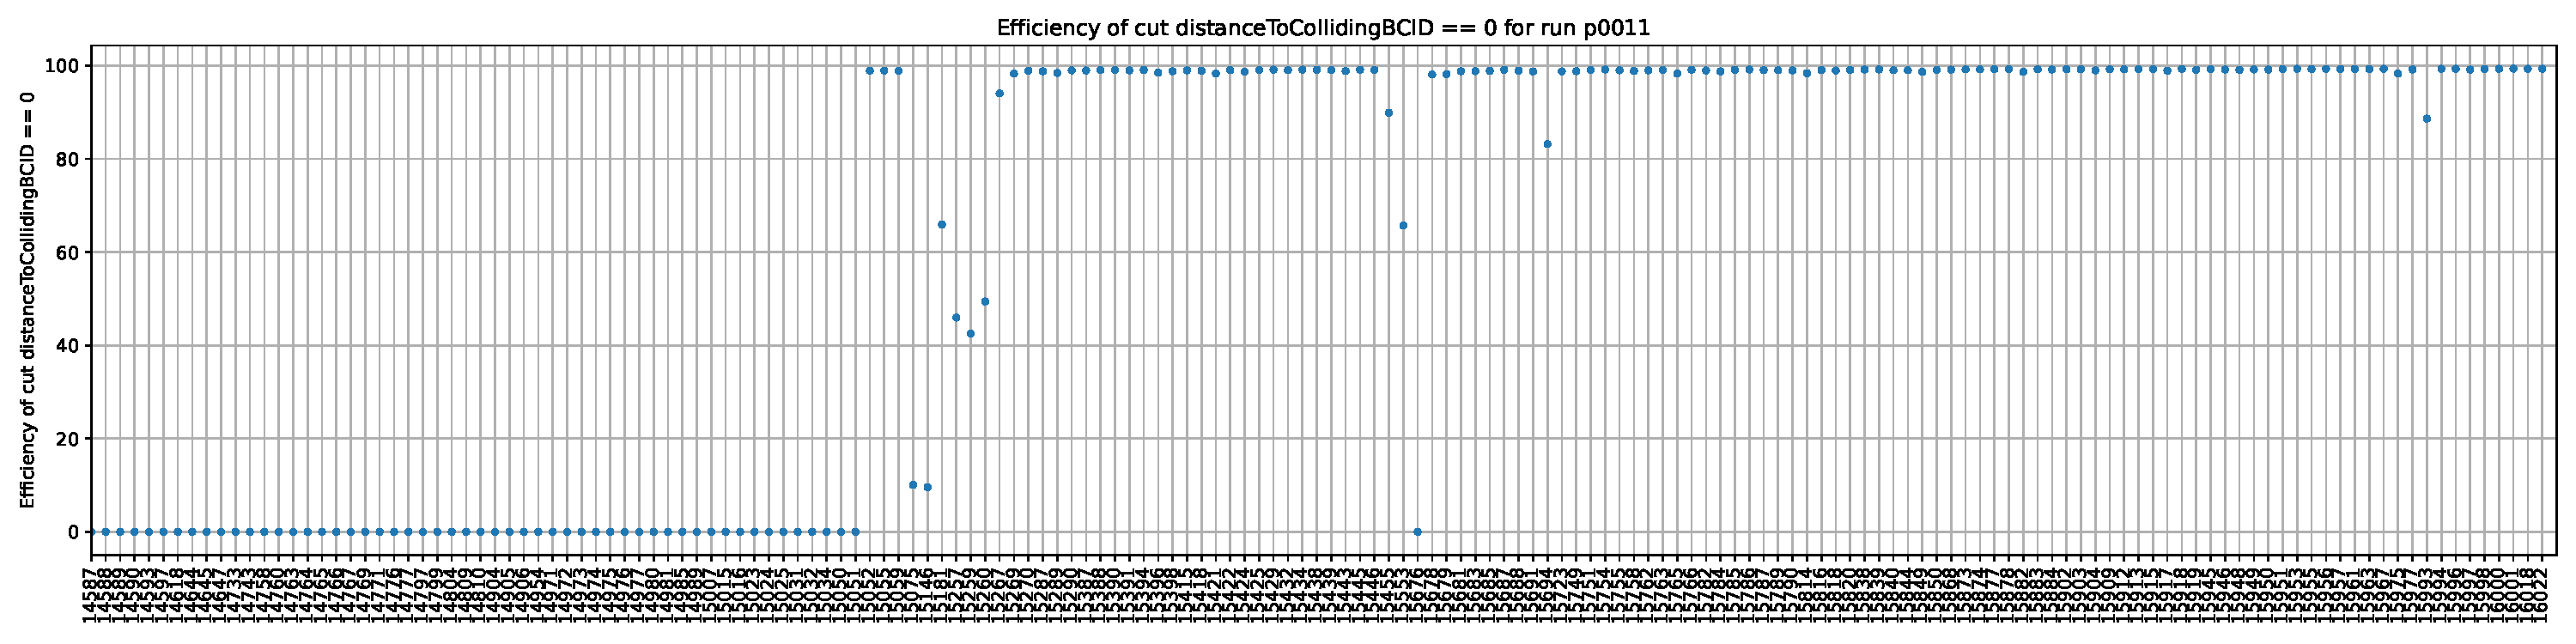
\includegraphics[width=\linewidth]{./assets/BCIDEfficiency_p0011.pdf}
		\caption{Efficiency of the BCID cut on the p0011 data}
	\end{figure}

\end{frame}

\begin{frame}{Yield Plots for F241-2024}
	\begin{center}
		\begin{tikzpicture}
			\node[anchor=south west, inner sep=0] (image) at (0,0) {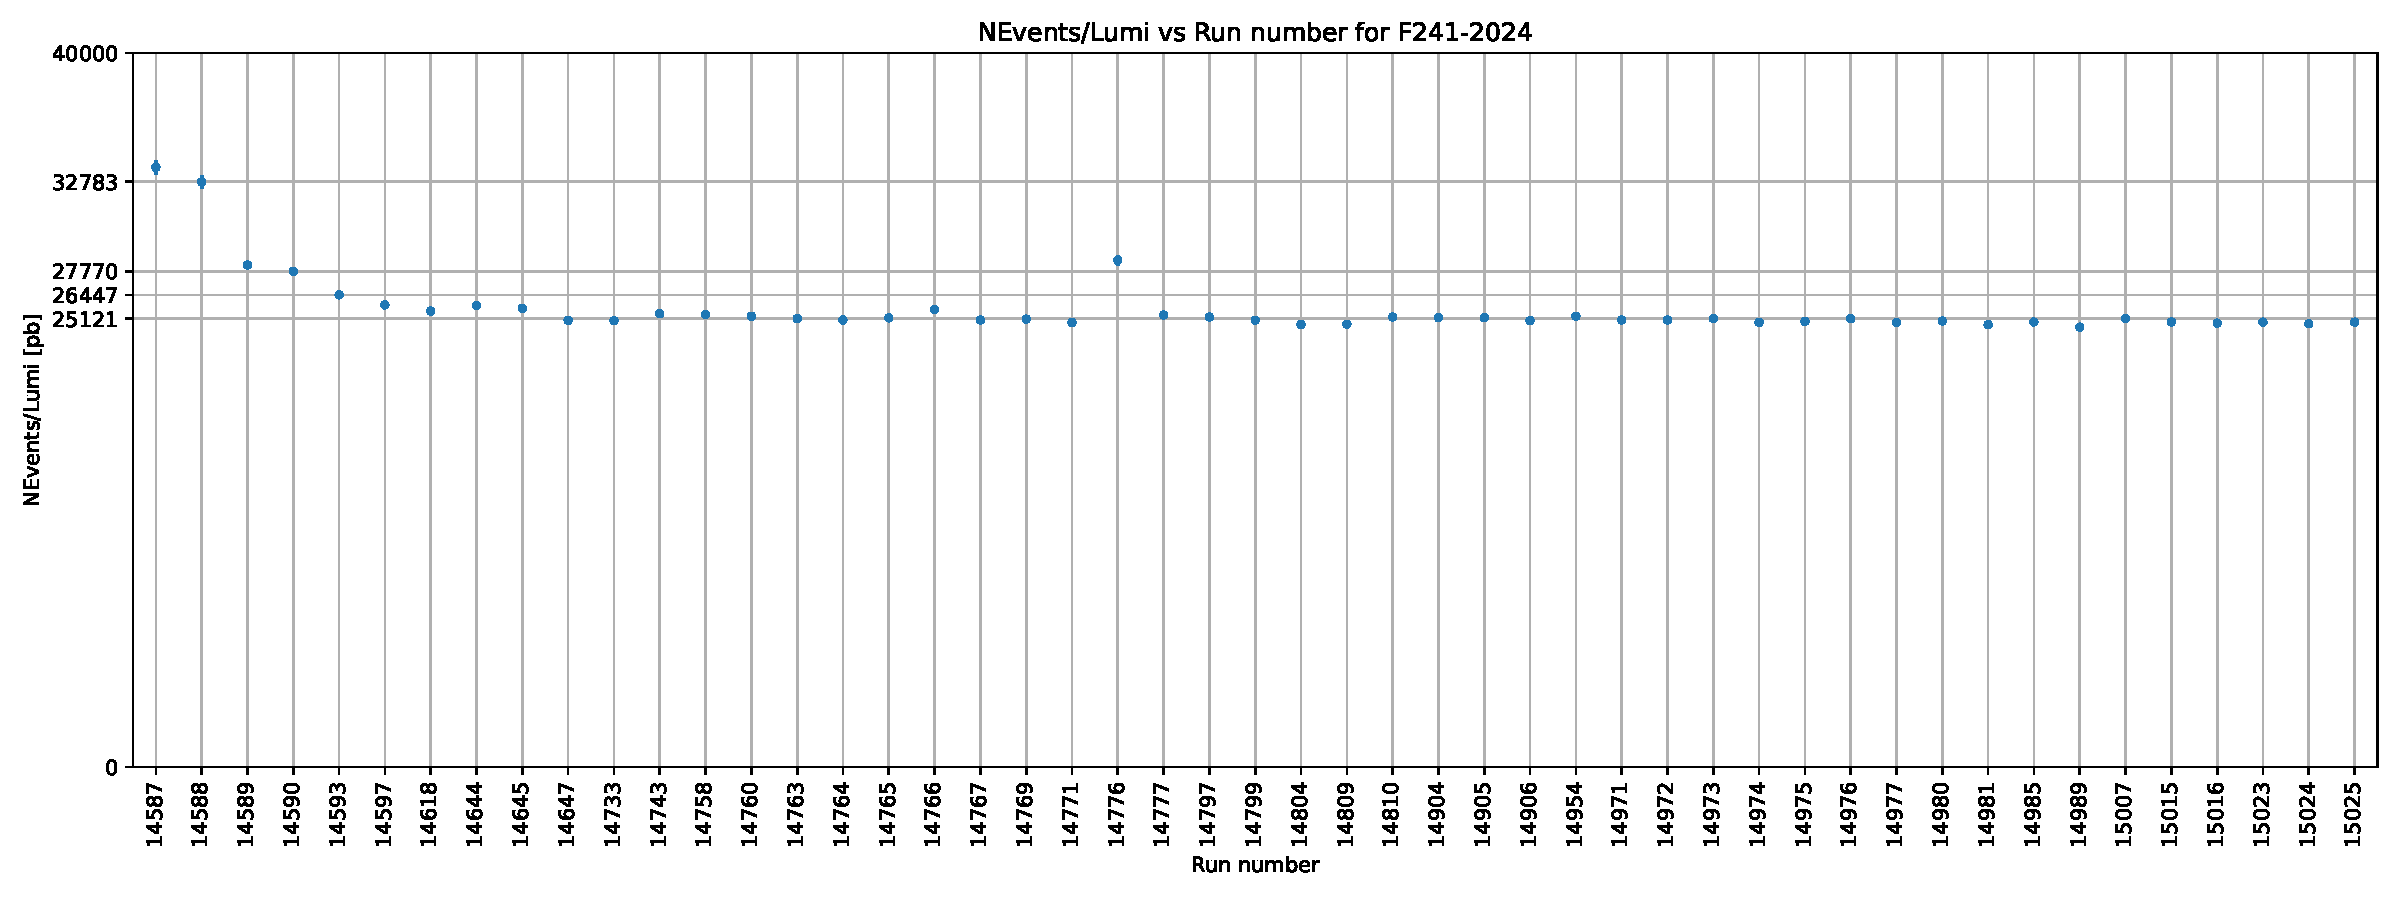
\includegraphics[height=0.4\textheight]{RunwisePlots/F241-2024_NEventsbyLumi.pdf}};
			\begin{scope}[x={(image.south east)},y={(image.north west)}]
				% \draw[help lines,xstep=.1,ystep=.1] (0,0) grid (1,1);
				\draw[red] (0.06,0.6) rectangle (0.25,0.84);
				\node[red, below, scale=0.6] at (0.155,0.6) {\tiny Early Runs Erratic};
				\draw[red] (0.455,0.69) rectangle (0.475,0.73);
				\node[red, right, scale=0.6] at (0.48,0.71) {\tiny Potentially Problematic [14776]};
			\end{scope}
		\end{tikzpicture}
	\end{center}
	\begin{center}
	\begin{tikzpicture}
		\centering
		\node[anchor=south west, inner sep=0] (image) at (0,0) {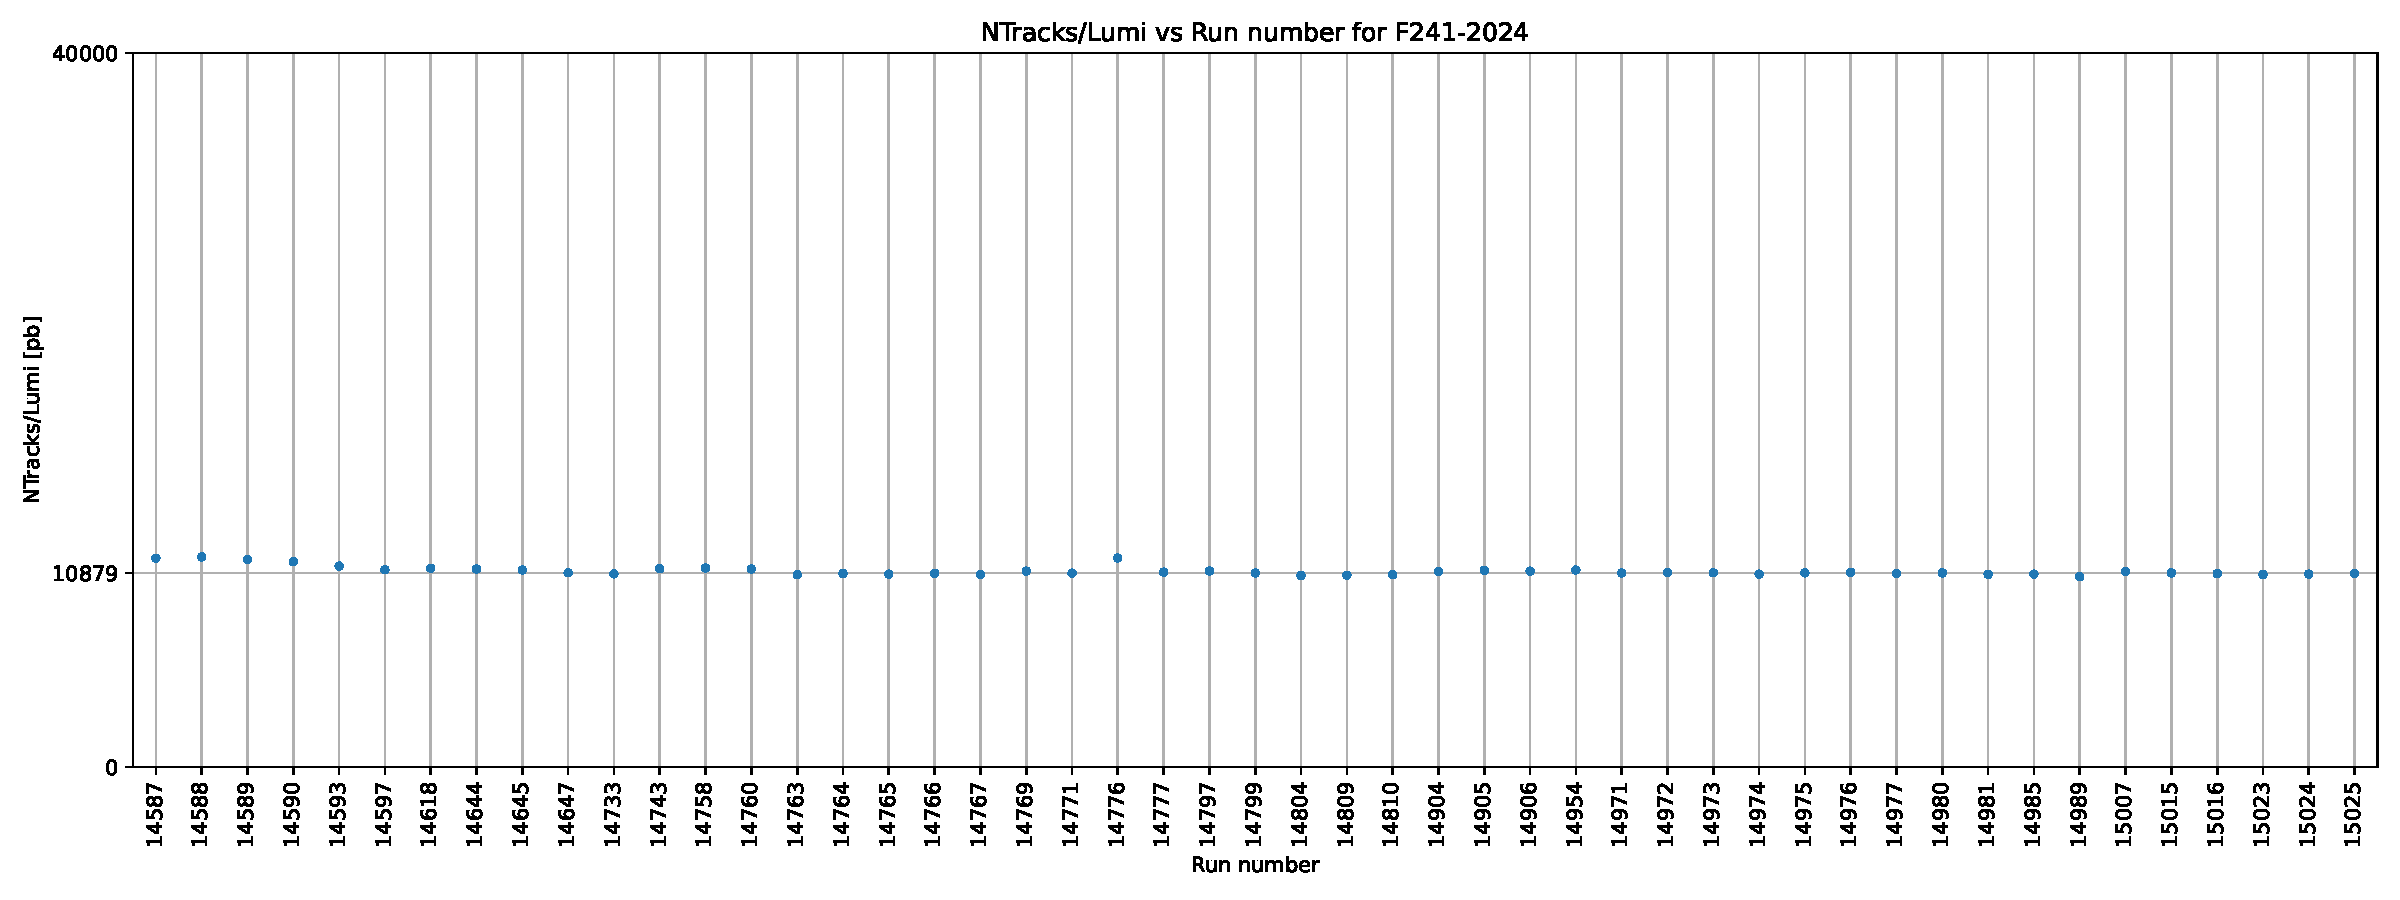
\includegraphics[height=0.4\textheight]{RunwisePlots/F241-2024_NTracksbyLumi.pdf}};
		\begin{scope}[x={(image.south east)},y={(image.north west)}]
			% \draw[help lines,xstep=.1,ystep=.1] (0,0) grid (1,1);
			\draw[red] (0.06,0.35) rectangle (0.25,0.4);
			\node[red, below, scale=0.6] at (0.155,0.36) {\tiny Less Pronounced!};
			\draw[red] (0.455,0.37) rectangle (0.475,0.4);
			% \node[red, right, scale=0.6] at (0.48,0.39) {\tiny Potentially Problematic [14776]};
		\end{scope}
	\end{tikzpicture}
\end{center}

\end{frame}

\begin{frame}{Yield Plots for Tungsten-2024}
	\begin{center}
	\begin{tikzpicture}
		\node[anchor=south west, inner sep=0] (image) at (0,0) {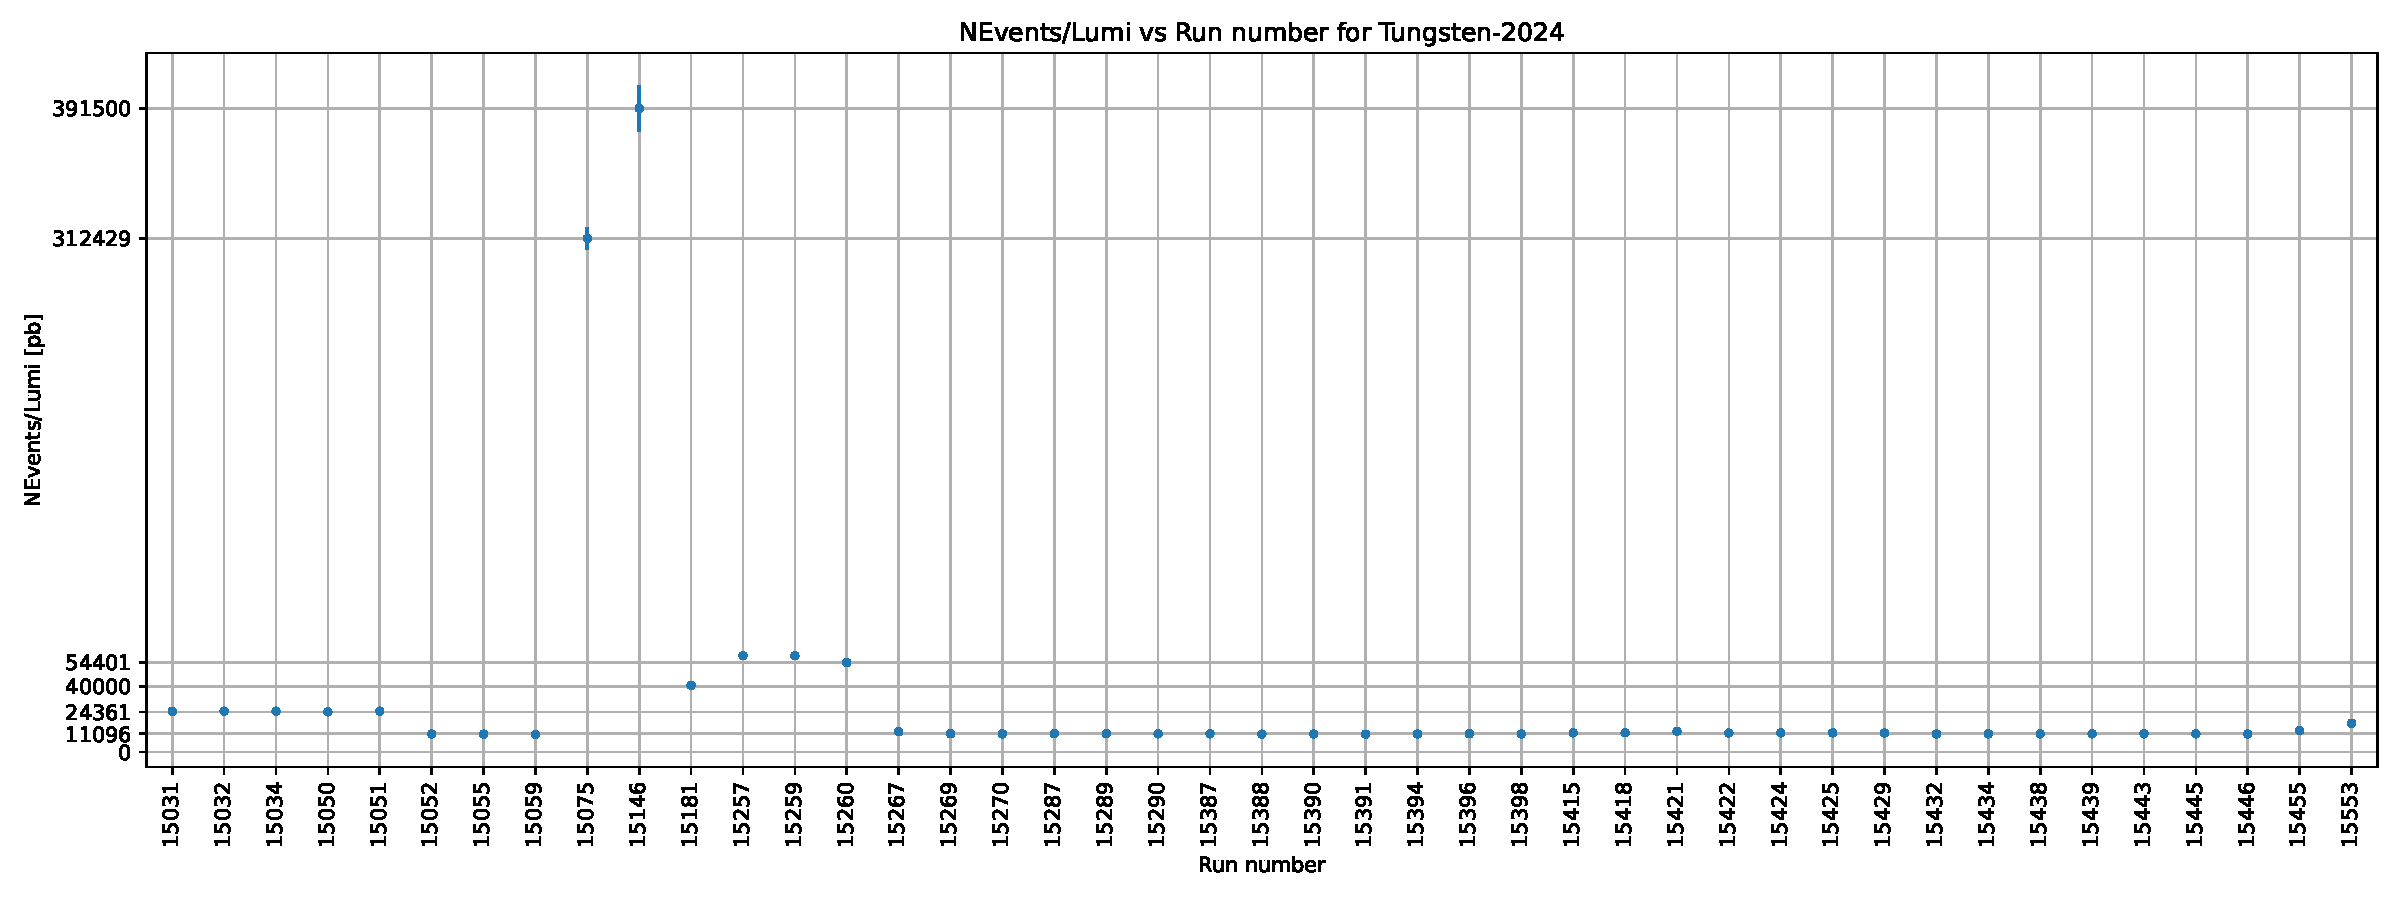
\includegraphics[height=0.4\textheight]{RunwisePlots/Tungsten-2024_NEventsbyLumi.pdf}};
		\begin{scope}[x={(image.south east)},y={(image.north west)}]
			% \draw[help lines,xstep=.1,ystep=.1] (0,0) grid (1,1);
			\draw[red] (0.065,0.198) rectangle (0.17,0.22);
			\node[red, above, scale=0.6] at (0.12,0.24) {\tiny Early Runs High?};
			\draw[red] (0.22,0.2) rectangle (0.37,0.93);
			\node[red, right, scale=0.6] at (0.37,0.6) {\tiny Unusually High! Throws off the scale};
			% \draw[red] (0.455,0.69) rectangle (0.475,0.73);
			% \node[red, right, scale=0.6] at (0.48,0.71) {\tiny Potentially Problematic [14776]};
		\end{scope}
	\end{tikzpicture}
	\end{center}
	\begin{center}
	\begin{tikzpicture}
		\node[anchor=south west, inner sep=0] (image) at (0,0) {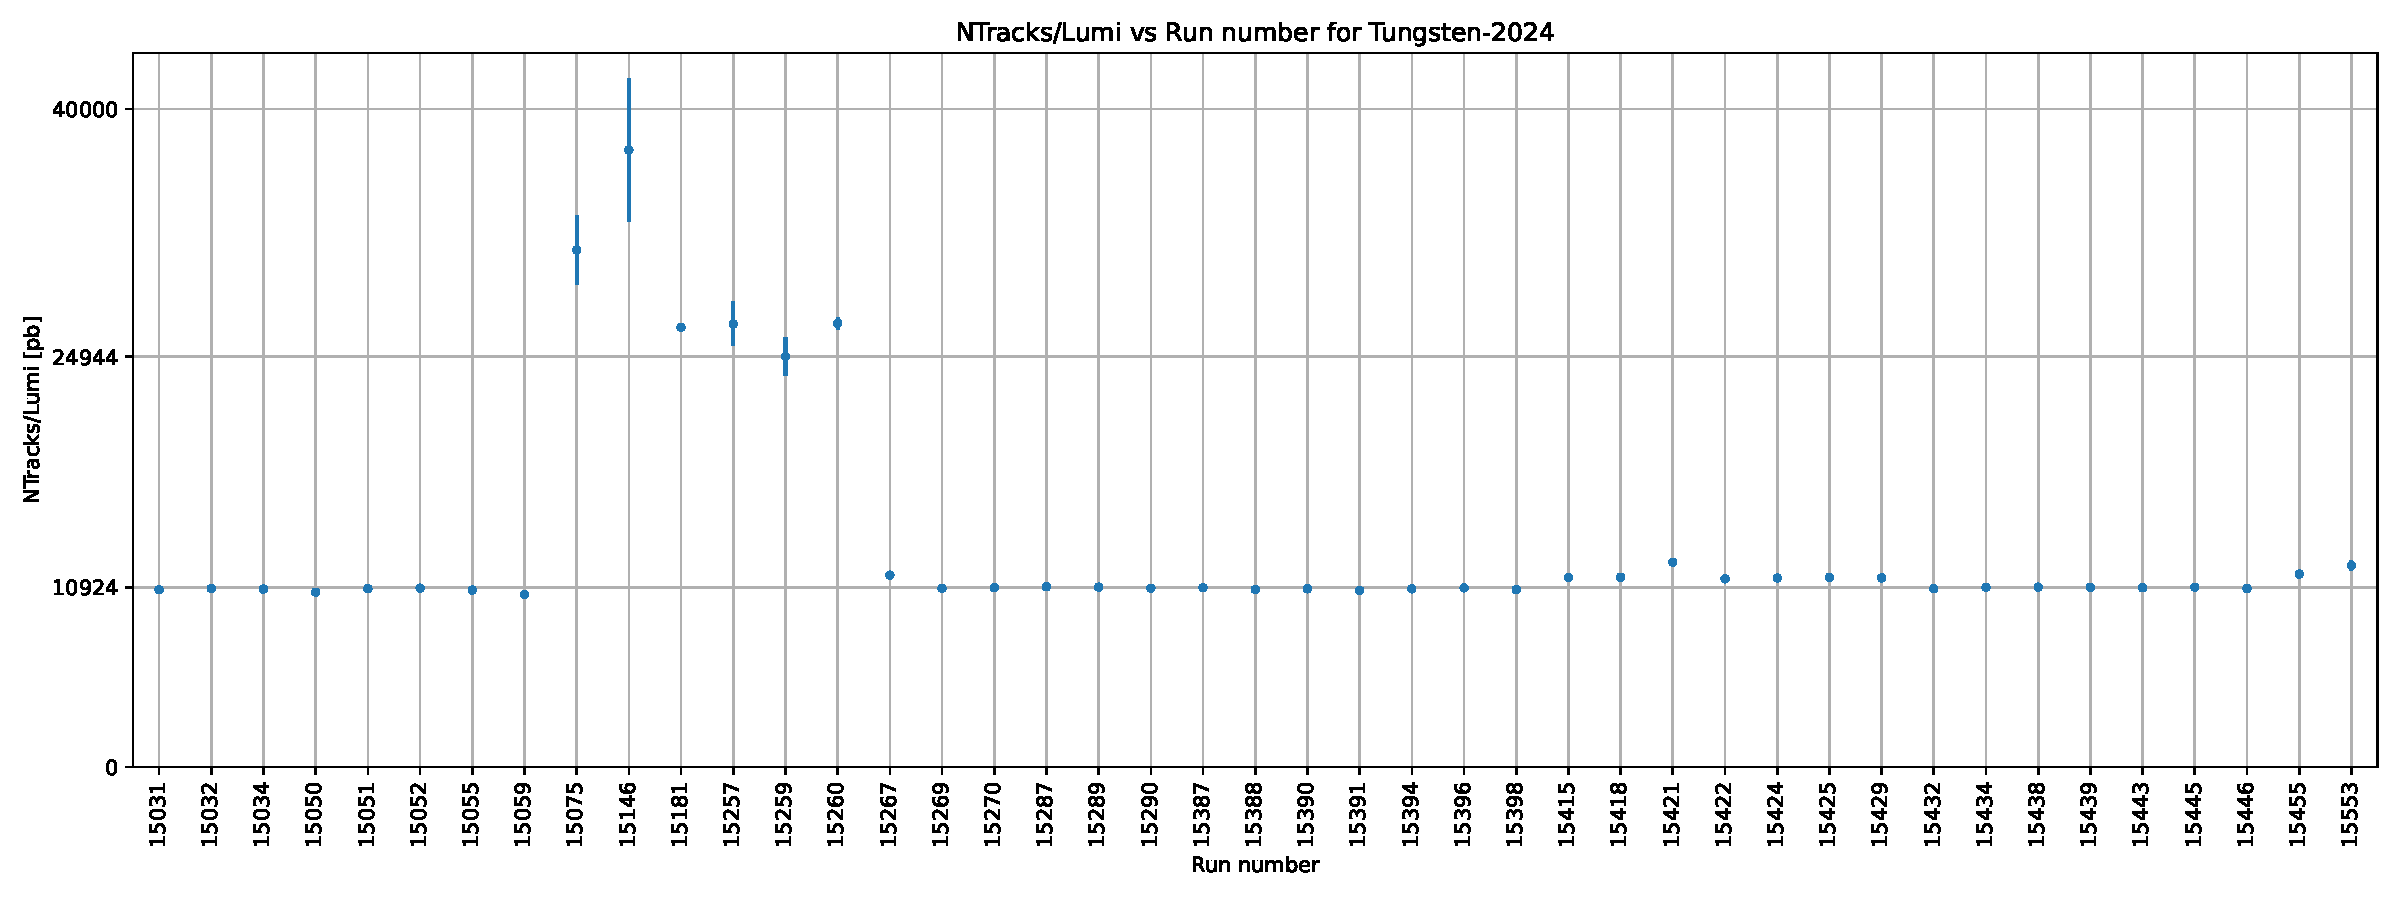
\includegraphics[height=0.4\textheight]{RunwisePlots/Tungsten-2024_NTracksbyLumi.pdf}};
		\begin{scope}[x={(image.south east)},y={(image.north west)}]
			% \draw[help lines,xstep=.1,ystep=.1] (0,0) grid (1,1);
			\draw[red] (0.062,0.335) rectangle (0.165,0.36);
			\node[red, above, scale=0.6] at (0.12,0.36) {\tiny Seem better here?};
			\draw[red] (0.22,0.45) rectangle (0.37,0.93);
			\node[red, right, scale=0.6] at (0.37,0.65) {\tiny Unusual!};
			\draw[red] (0.64,0.35) rectangle (0.8,0.4);
			\draw[red] (0.95,0.35) rectangle (0.99,0.4);
			\draw[red] (0.8,0.4) -- (0.95,0.4);
			\node[red, right, scale=0.6] at (0.83,0.43) {\tiny Slightly Elevated?};
		\end{scope}
	\end{tikzpicture}
\end{center}
\end{frame}

\begin{frame}{Yield Plots for F242-2024}
\begin{center}
	\begin{tikzpicture}
		\node[anchor=south west, inner sep=0] (image) at (0,0) {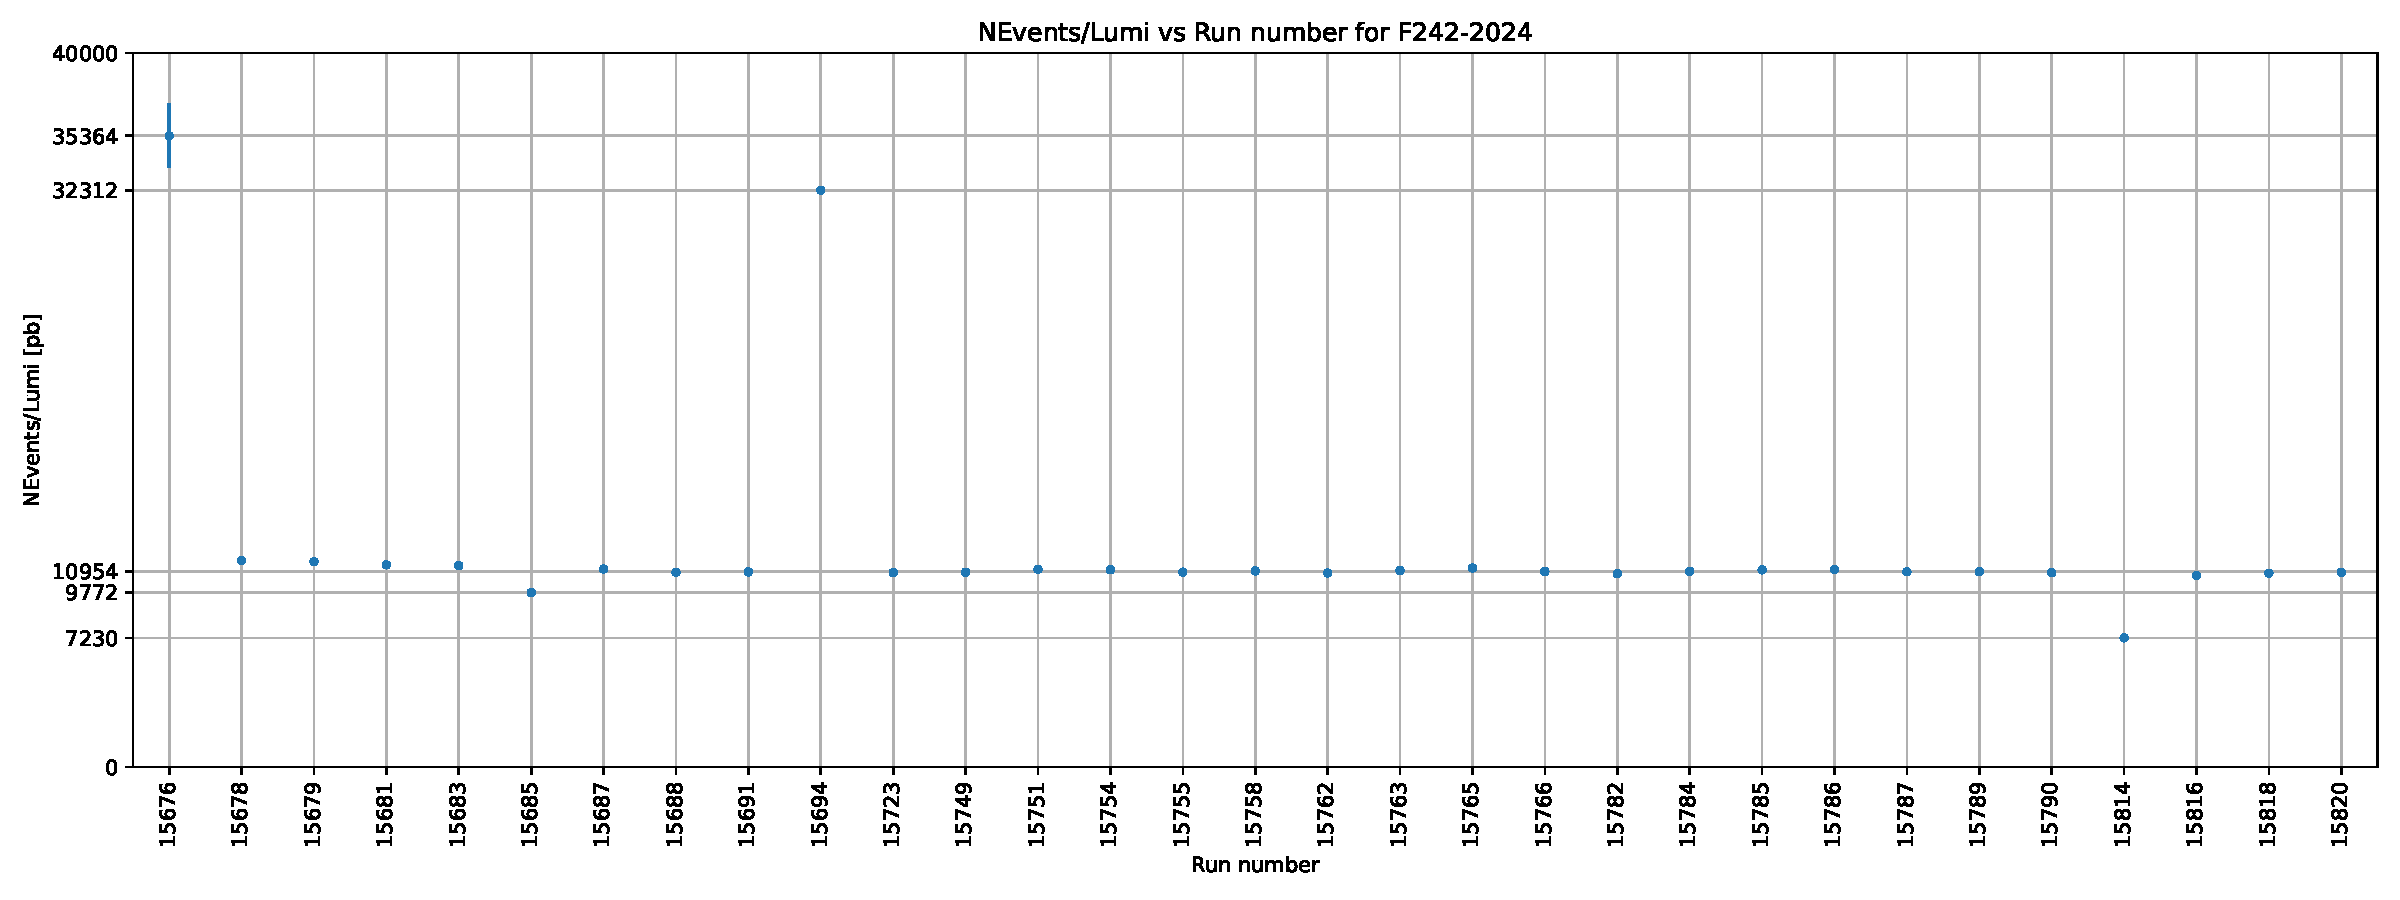
\includegraphics[height=0.4\textheight]{RunwisePlots/F242-2024_NEventsbyLumi.pdf}};
		\begin{scope}[x={(image.south east)},y={(image.north west)}]
			% \draw[help lines,xstep=.1,ystep=.1] (0,0) grid (1,1);
			\draw[red] (0.06,0.8) rectangle (0.08,0.9);
			\node[red, right, scale=0.6] at (0.08,0.85) {\tiny High};
			\draw[red] (0.335,0.76) rectangle (0.35,0.82);
			\node[red, right, scale=0.6] at (0.35,0.80) {\tiny  High};
			\draw[red] (0.215,0.32) rectangle (0.23,0.355);
			\node[red, below, scale=0.6] at (0.225,0.34) {\tiny  Low?};
			\draw[red] (0.879,0.275) rectangle (0.89,0.31);
			\node[red, below, scale=0.6] at (0.885,0.275) {\tiny  Low};
		\end{scope}
	\end{tikzpicture}
\end{center}
\begin{center}
	\begin{tikzpicture}
		\node[anchor=south west, inner sep=0] (image) at (0,0) {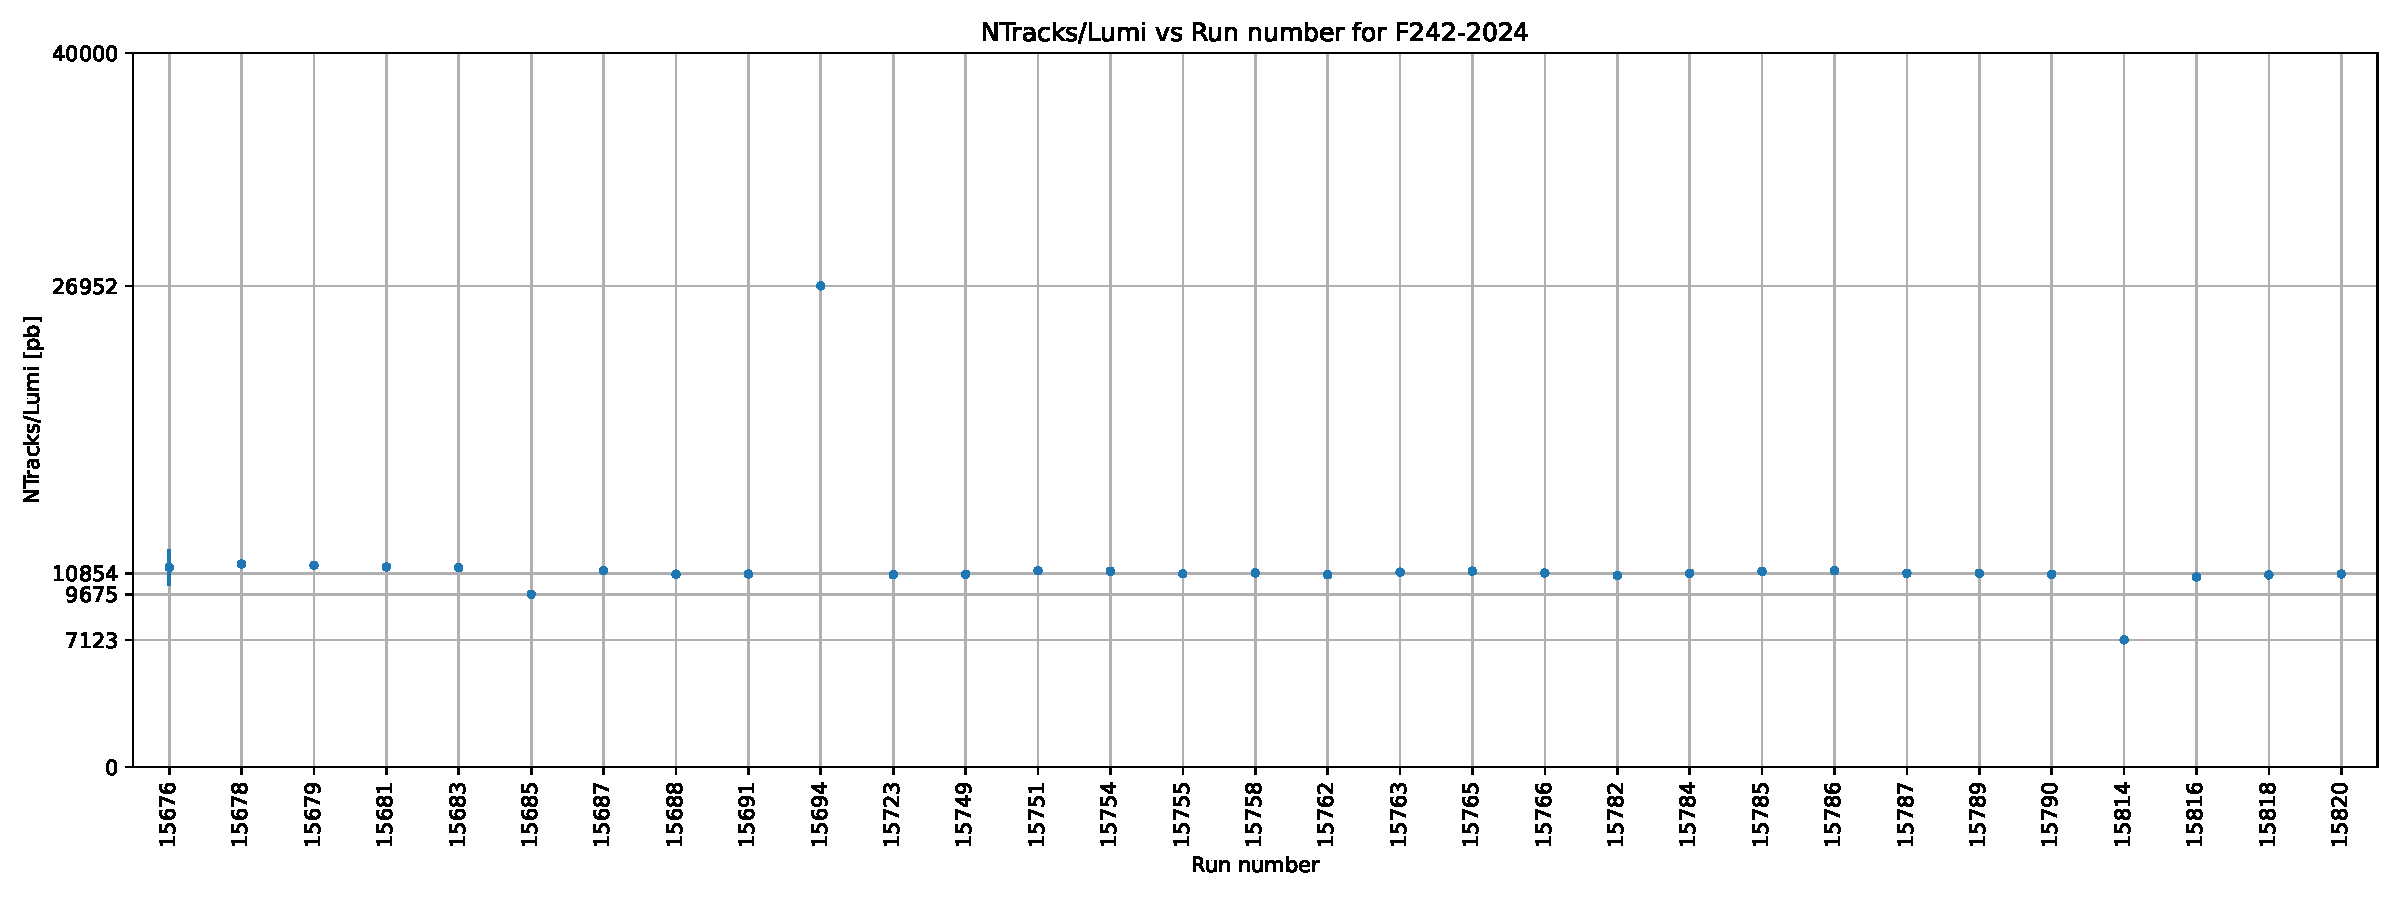
\includegraphics[height=0.4\textheight]{RunwisePlots/F242-2024_NTracksbyLumi.pdf}};
		\begin{scope}[x={(image.south east)},y={(image.north west)}]
			% \draw[help lines,xstep=.1,ystep=.1] (0,0) grid (1,1);
			\draw[red] (0.06,0.34) rectangle (0.2,0.4);
			\node[red, above, scale=0.6] at (0.13,0.4) {\tiny Slightly Elevated};
			\draw[red] (0.335,0.65) rectangle (0.35,0.7);
			\node[red, above, scale=0.6] at (0.3425,0.7) {\tiny  High};
			\draw[red] (0.215,0.32) rectangle (0.23,0.355);
			\node[red, below, scale=0.6] at (0.225,0.34) {\tiny  Low?};
			\draw[red] (0.879,0.275) rectangle (0.89,0.31);
			\node[red, below, scale=0.6] at (0.885,0.275) {\tiny  Low};
		\end{scope}
	\end{tikzpicture}
\end{center}

\end{frame}

\begin{frame}{Yield Plots for CaloNu-2024}
\begin{center}
	\begin{tikzpicture}
		\node[anchor=south west, inner sep=0] (image) at (0,0) {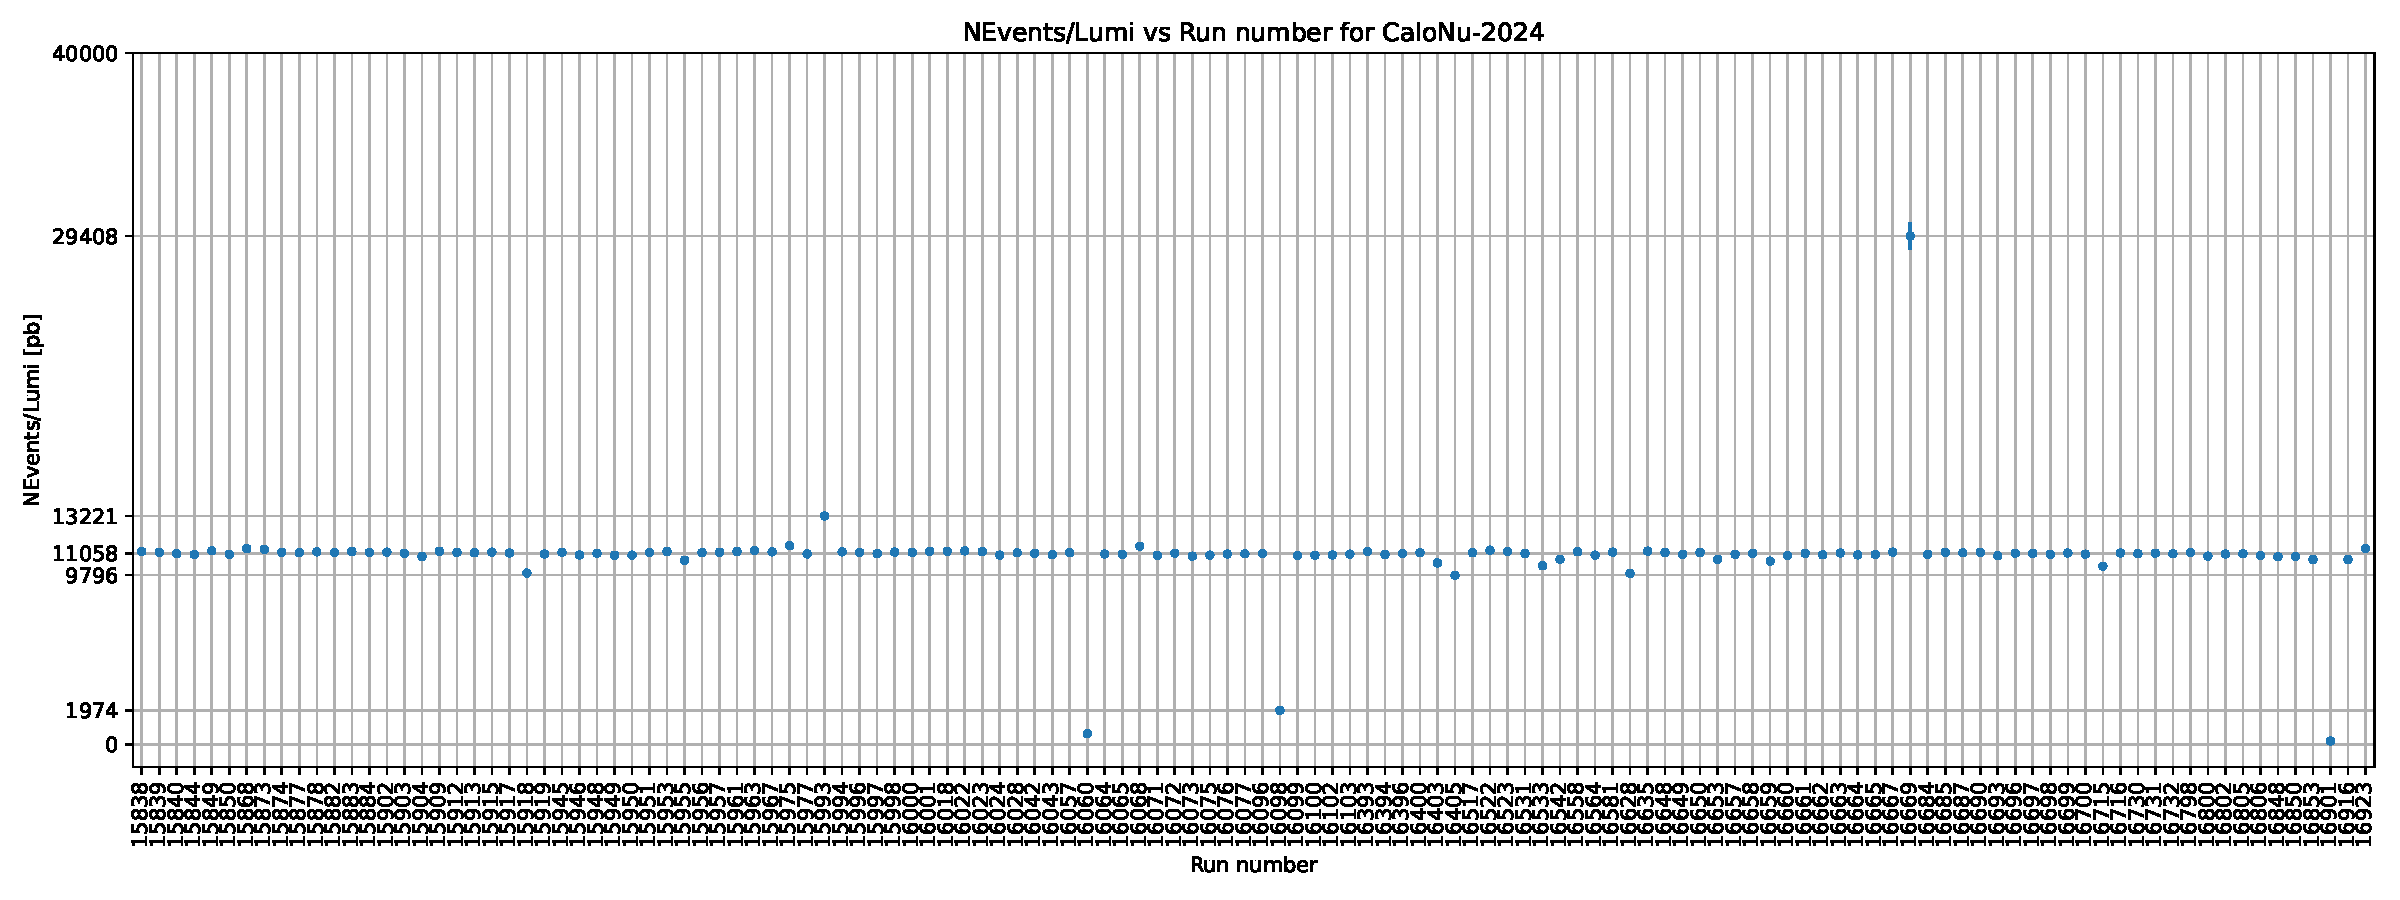
\includegraphics[height=0.4\textheight]{RunwisePlots/CaloNu-2024_NEventsbyLumi.pdf}};
		\begin{scope}[x={(image.south east)},y={(image.north west)}]
			% \draw[help lines,xstep=.05,ystep=.05] (0,0) grid (1,1);
			% \foreach \x in {0,1,...,9} { \node [anchor=north] at (\x/10,0) {0.\x}; }
			% \foreach \y in {0,1,...,9} { \node [anchor=east] at (0,\y/10) {0.\y}; }
			\draw[red] (0.78,0.71) rectangle (0.81,0.76);
			\node[red, above, scale=0.6] at (0.795,0.76) {\tiny High};
			\draw[red] (0.335,0.41) rectangle (0.35,0.45);
			\node[red, above, scale=0.6] at (0.3425,0.45) {\tiny High?};
			\draw[red] (0.215,0.35) rectangle (0.225,0.375);
			\draw[red] (0.595,0.35) rectangle (0.61,0.38);
			\draw[red] (0.639,0.358) rectangle (0.655,0.385);
			\draw[red] (0.675,0.35) rectangle (0.683,0.373);
			\draw[red] (0.872,0.36) rectangle (0.88,0.38);
			\draw[red] (0.445,0.17) rectangle (0.46,0.2);
			\node[red, above, scale=0.6] at (0.495, 0.19) {\tiny Low};
			\draw[red] (0.525,0.2) rectangle (0.54,0.22);
			\draw[red] (0.965,0.16) rectangle (0.975,0.19);
			\node[red, above, scale=0.6] at (0.97,0.19) {\tiny Low};
		\end{scope}
	\end{tikzpicture}
\end{center}
\begin{center}
	\begin{tikzpicture}
		\node[anchor=south west, inner sep=0] (image) at (0,0) {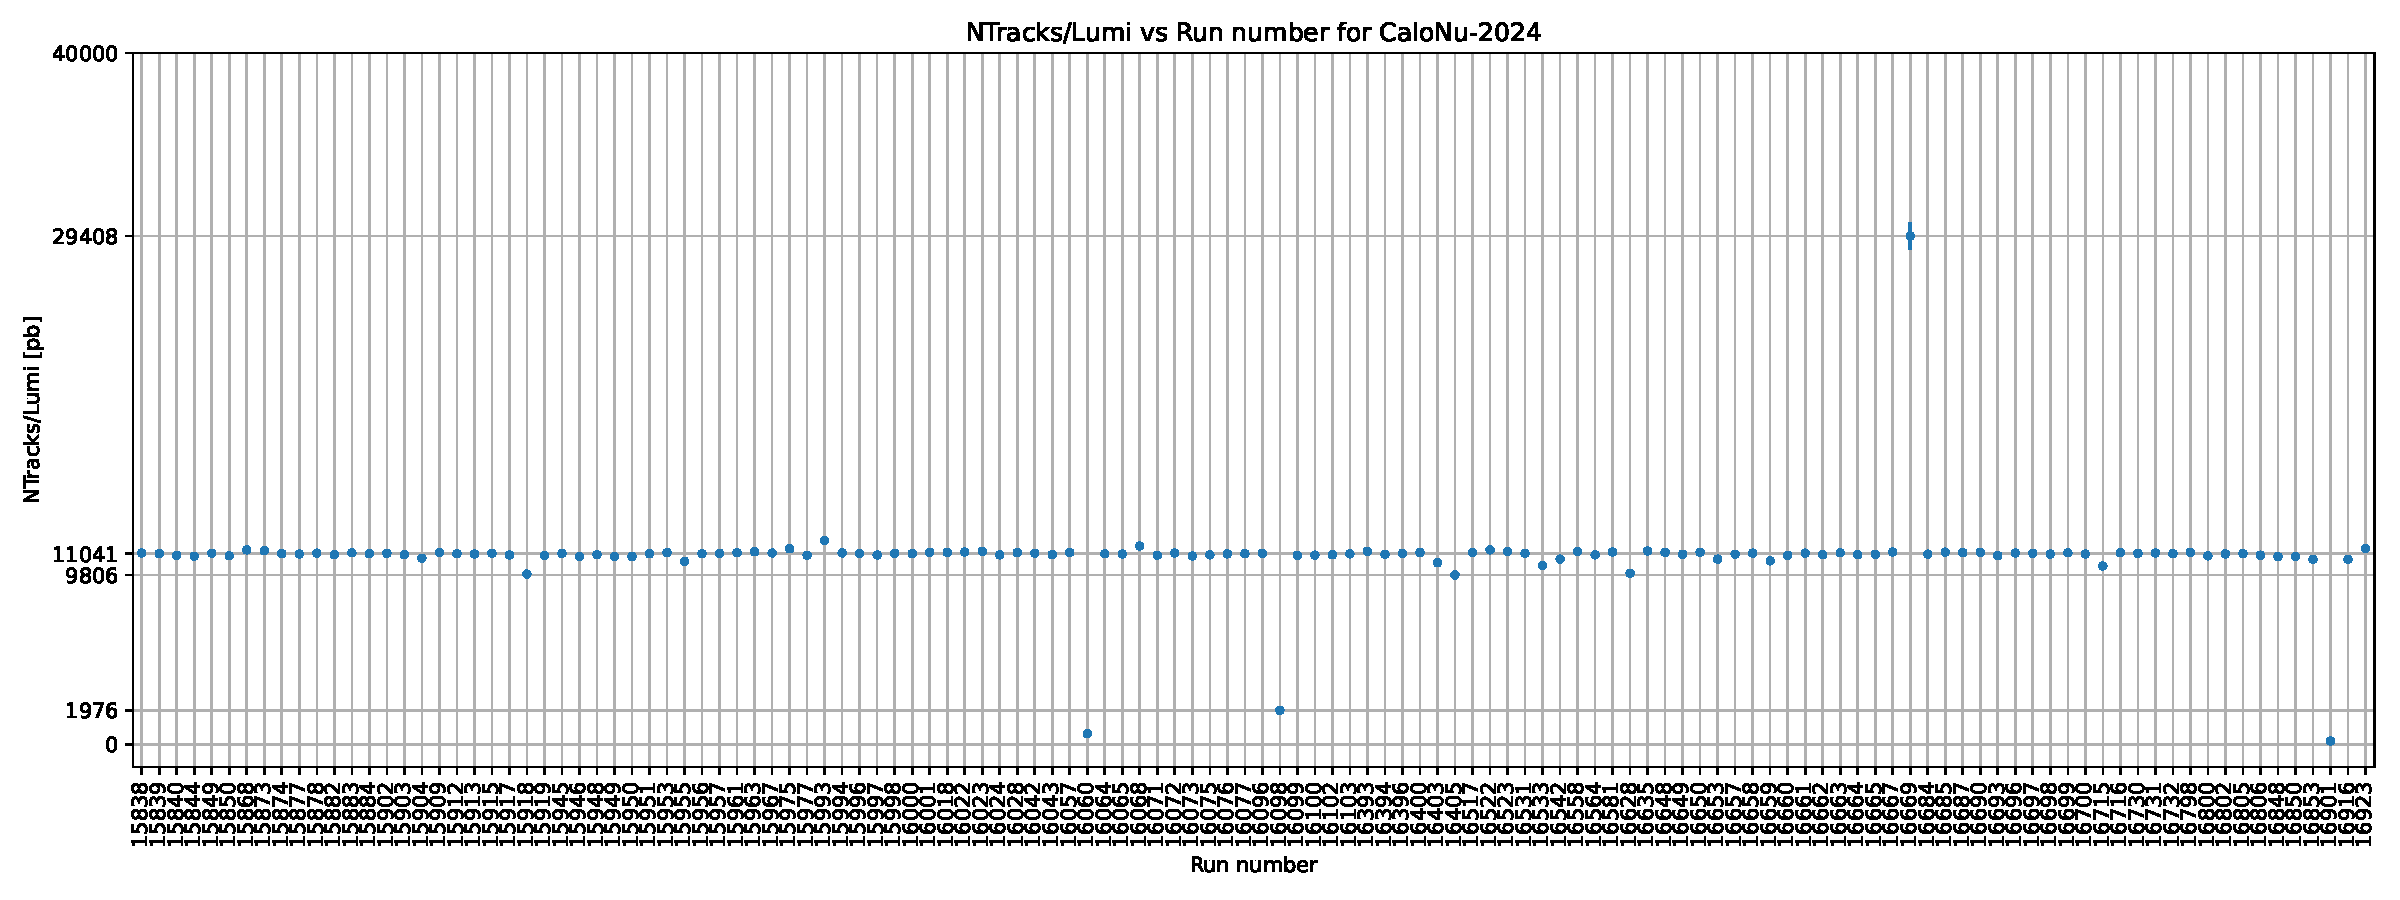
\includegraphics[height=0.4\textheight]{RunwisePlots/CaloNu-2024_NTracksbyLumi.pdf}};
		\begin{scope}[x={(image.south east)},y={(image.north west)}]
			\draw[red] (0.78,0.71) rectangle (0.81,0.76);
			\node[red, above, scale=0.6] at (0.795,0.76) {\tiny High};
			\draw[red] (0.3375,0.39) rectangle (0.35,0.41);
			\node[red, above, scale=0.6] at (0.3475,0.41) {\tiny Better?};
			\draw[red] (0.215,0.35) rectangle (0.225,0.375);
			\draw[red] (0.595,0.35) rectangle (0.61,0.38);
			\draw[red] (0.639,0.358) rectangle (0.655,0.385);
			\draw[red] (0.675,0.35) rectangle (0.683,0.373);
			\draw[red] (0.872,0.36) rectangle (0.88,0.38);
			\draw[red] (0.445,0.17) rectangle (0.46,0.2);
			\node[red, above, scale=0.6] at (0.495, 0.19) {\tiny Low};
			\draw[red] (0.525,0.2) rectangle (0.54,0.22);
			\draw[red] (0.965,0.16) rectangle (0.975,0.19);
			\node[red, above, scale=0.6] at (0.97,0.19) {\tiny Low};
		\end{scope}
	\end{tikzpicture}
\end{center}
\end{frame}

\begin{frame}{Yield Plots for F243-2024}
	\begin{center}
	\begin{tikzpicture}
		\node[anchor=south west, inner sep=0] (image) at (0,0) {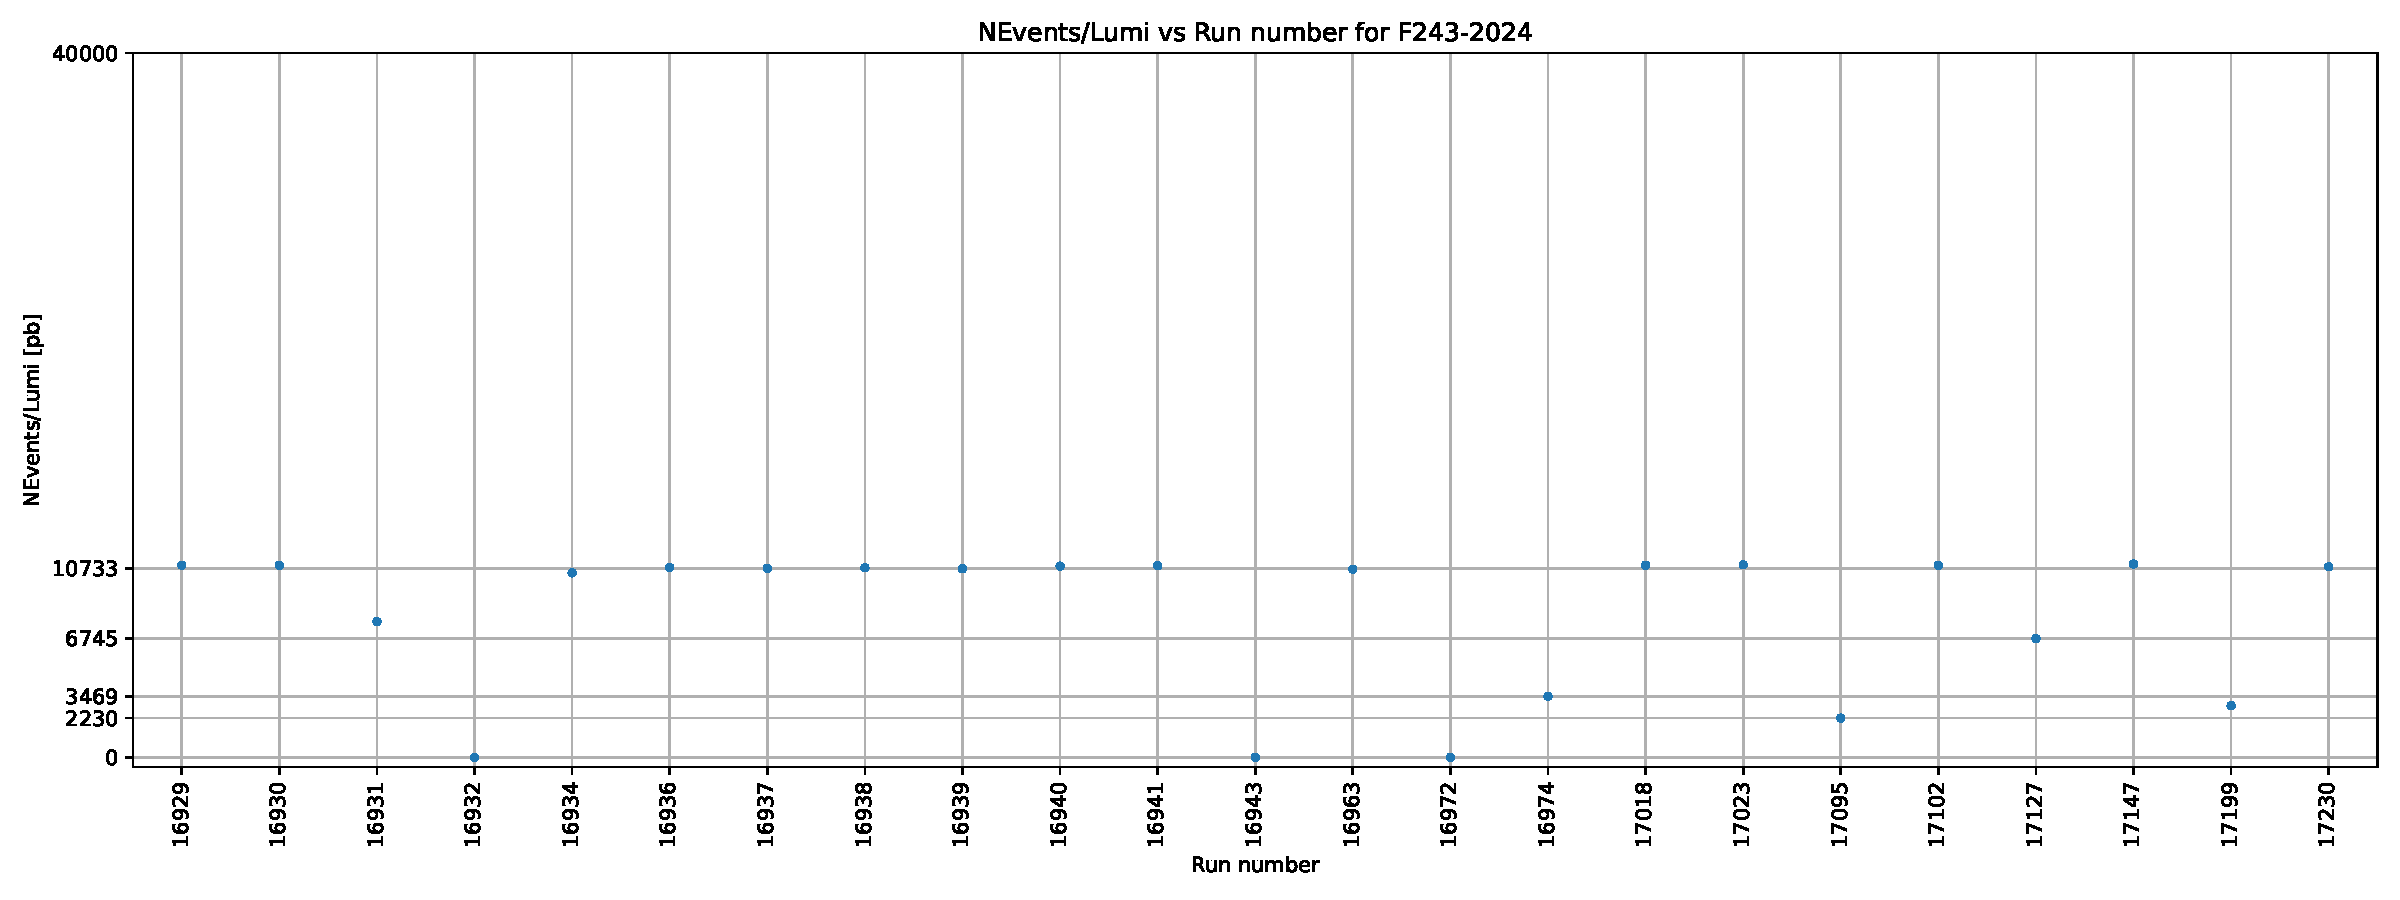
\includegraphics[height=0.4\textheight]{RunwisePlots/F243-2024_NEventsbyLumi.pdf}};
		\begin{scope}[x={(image.south east)},y={(image.north west)}]
			% \draw[help lines,xstep=.1,ystep=.1] (0,0) grid (1,1);
			\draw[red] (0.15,0.29) rectangle (0.165,0.33);
			\draw[red] (0.19,0.15) rectangle (0.205,0.17);
			\node[red, above, scale=0.6] at (0.1975,0.16) {\tiny Zero!};
			\draw[red] (0.515,0.15) rectangle (0.53,0.17);
			\draw[red] (0.598,0.15) rectangle (0.61,0.17);
			\node[red, above, scale=0.6] at (0.564,0.15) {\tiny Zero!};
			\draw[red] (0.64,0.2) rectangle (0.65,0.25);
			\draw[red] (0.76,0.18) rectangle (0.773,0.22);
			\draw[red] (0.84,0.28) rectangle (0.854,0.3);
			\draw[red] (0.925,0.205) rectangle (0.935,0.23);
		\end{scope}
	\end{tikzpicture}
\end{center}
	\begin{center}
	\begin{tikzpicture}
		\node[anchor=south west, inner sep=0] (image) at (0,0) {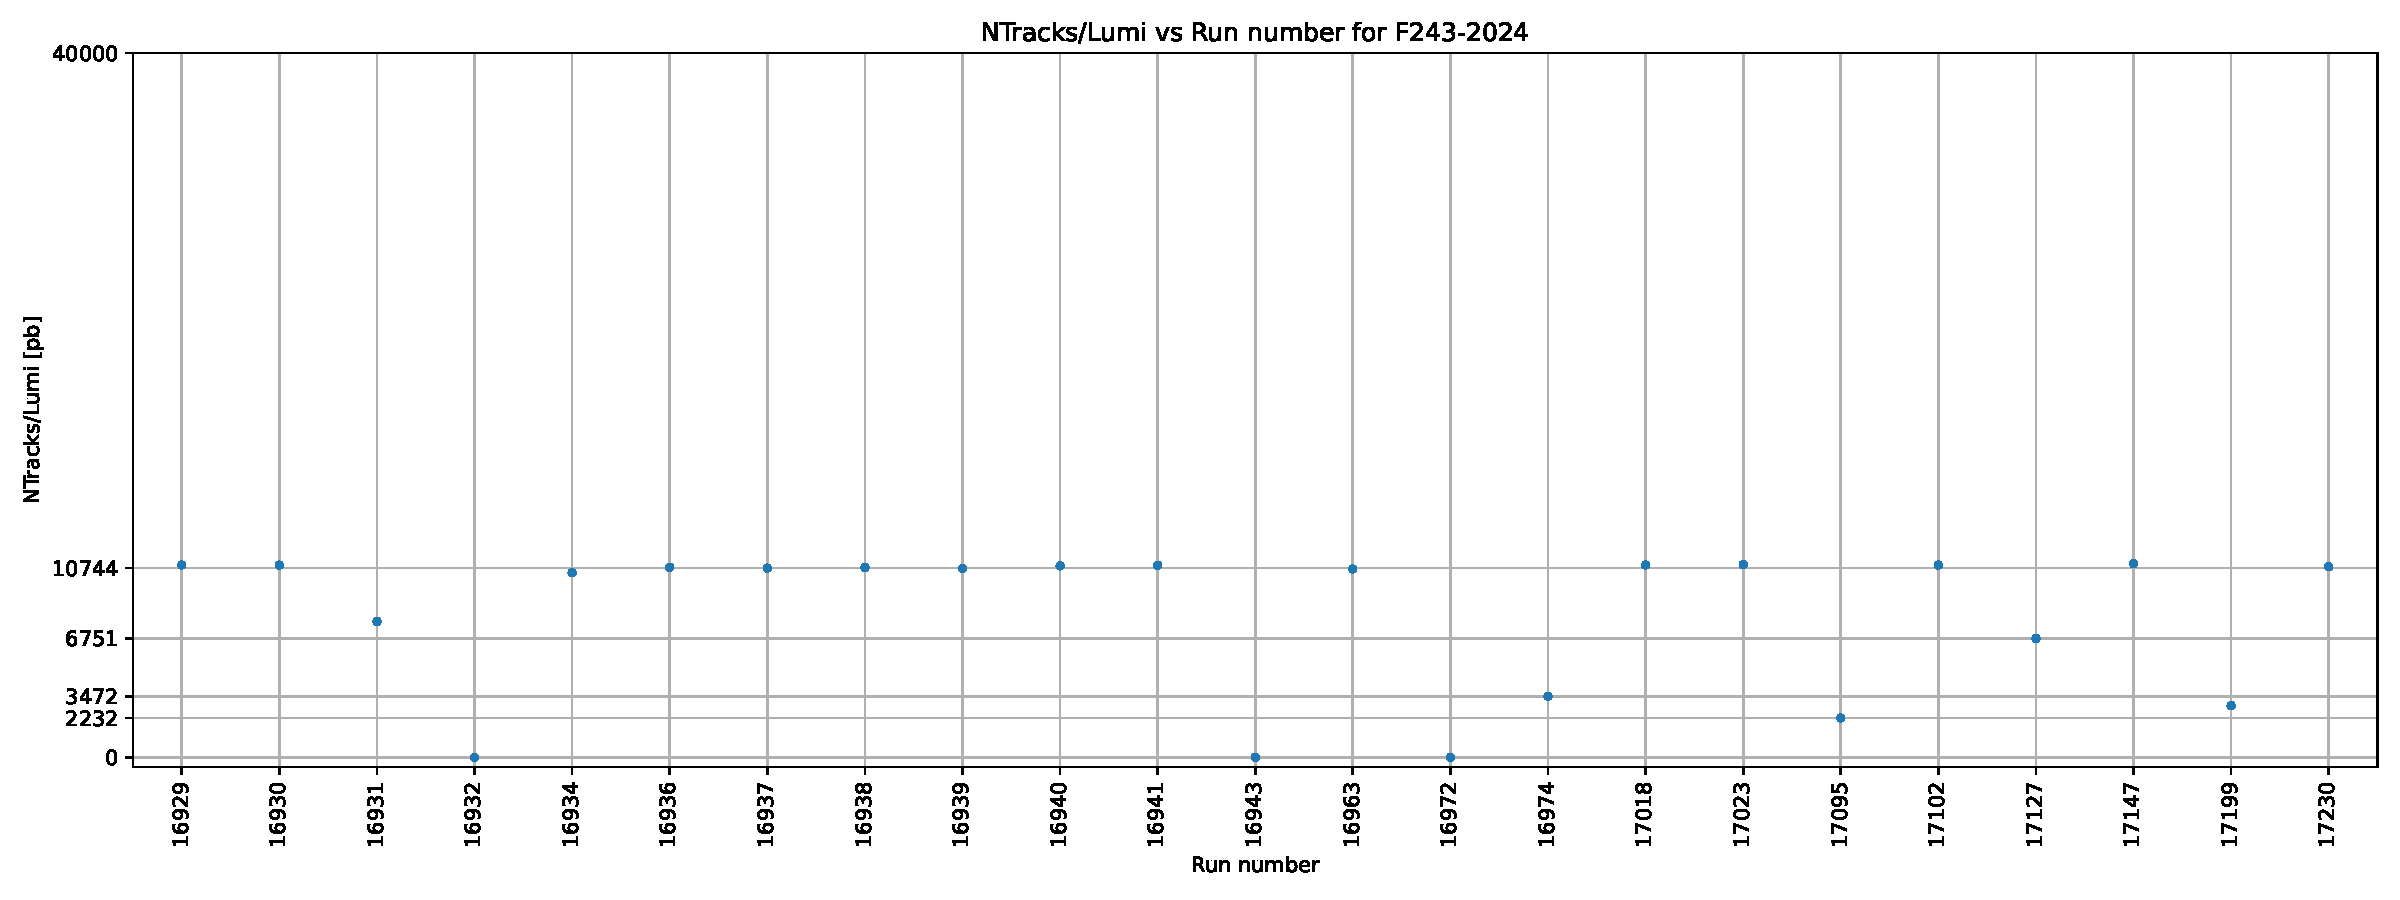
\includegraphics[height=0.4\textheight]{RunwisePlots/F243-2024_NTracksbyLumi.pdf}};
		\begin{scope}[x={(image.south east)},y={(image.north west)}]
			% \draw[help lines,xstep=.1,ystep=.1] (0,0) grid (1,1);
			\draw[red] (0.15,0.29) rectangle (0.165,0.33);
			\draw[red] (0.19,0.15) rectangle (0.205,0.17);
			\node[red, above, scale=0.6] at (0.1975,0.16) {\tiny Zero!};
			\draw[red] (0.515,0.15) rectangle (0.53,0.17);
			\draw[red] (0.598,0.15) rectangle (0.61,0.17);
			\node[red, above, scale=0.6] at (0.564,0.15) {\tiny Zero!};
			\draw[red] (0.64,0.2) rectangle (0.65,0.25);
			\draw[red] (0.76,0.18) rectangle (0.773,0.22);
			\draw[red] (0.84,0.28) rectangle (0.854,0.3);
			\draw[red] (0.925,0.205) rectangle (0.935,0.23);
		\end{scope}
	\end{tikzpicture}
	\end{center}
\end{frame}



% \begin{frame}{Yield Plots for F241-2024}
% 	\begin{figure}
% 		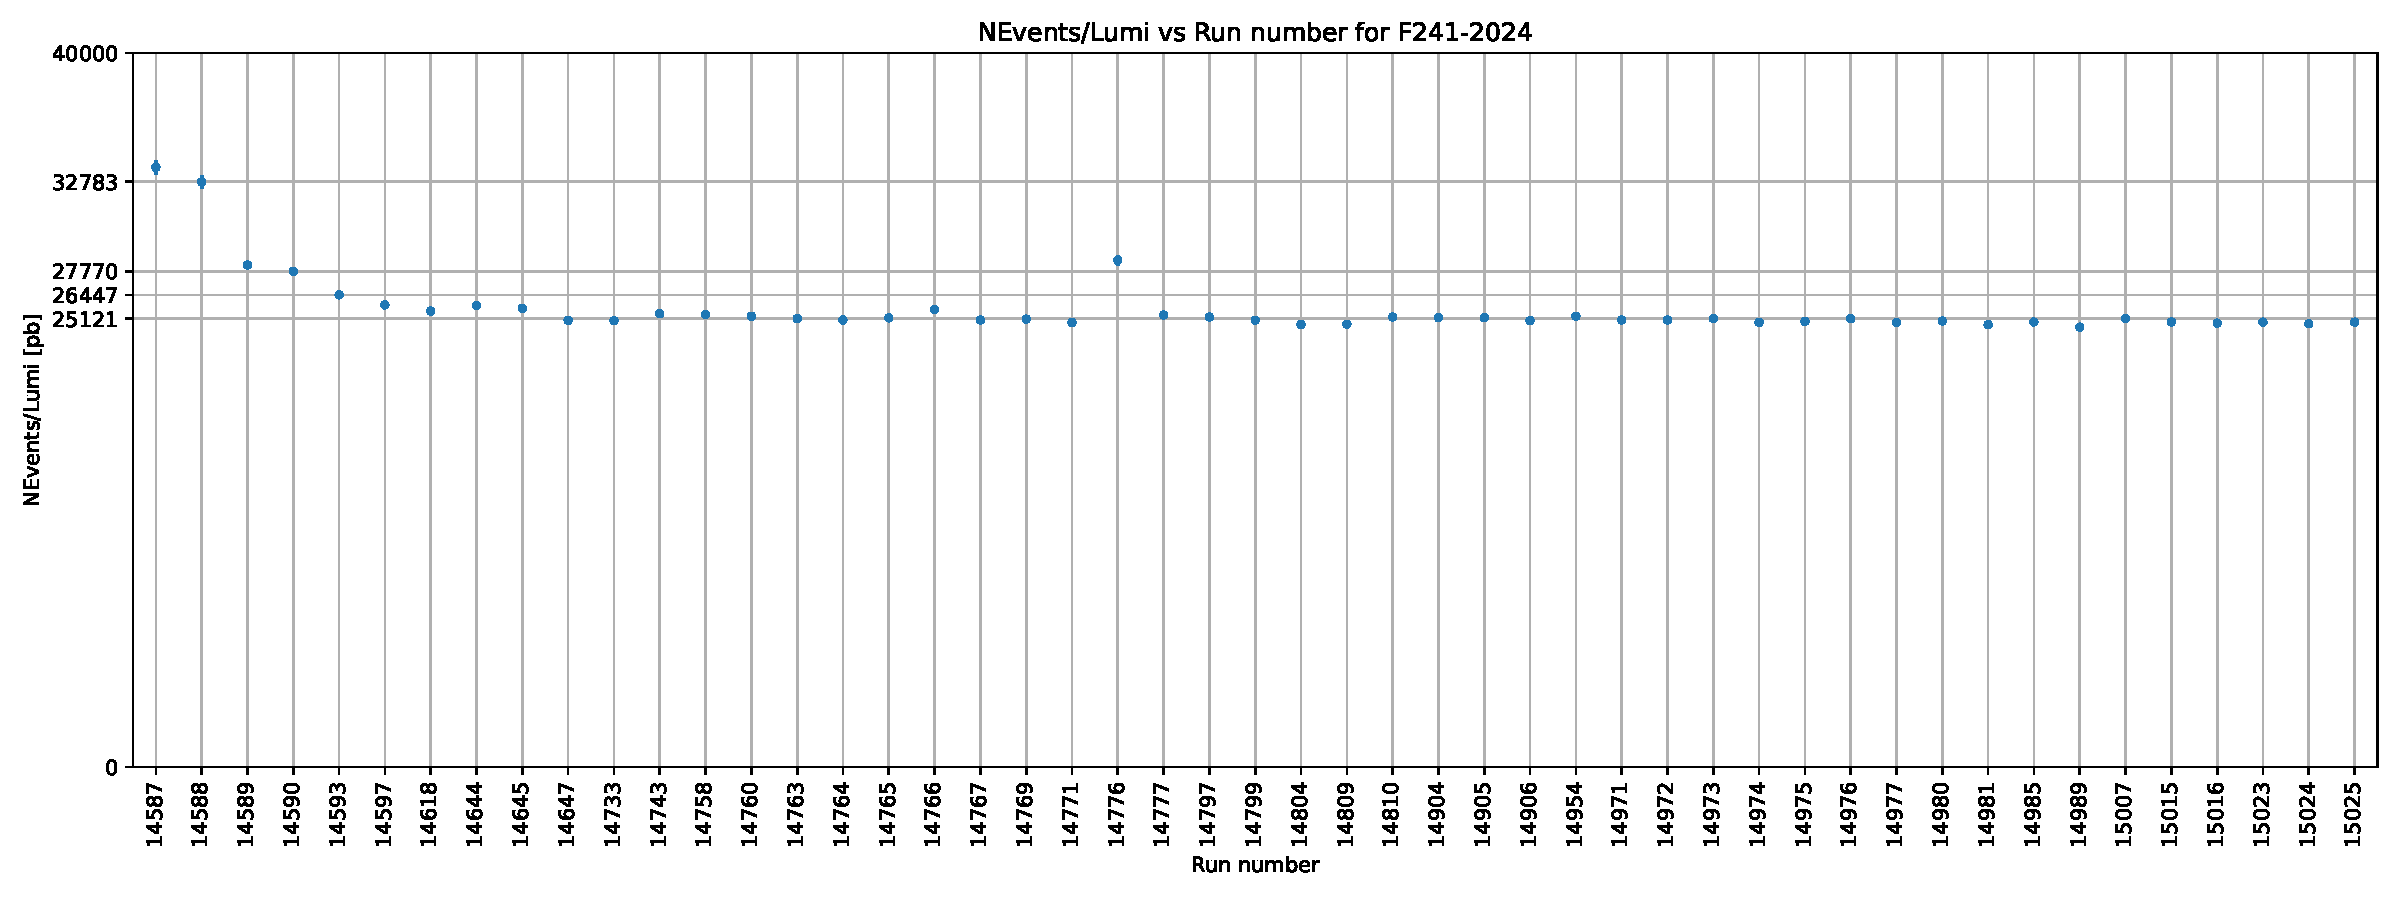
\includegraphics[height=0.4\textheight]{RunwisePlots/F241-2024_NEventsbyLumi.pdf}
% 	\end{figure}
% 	\begin{figure}
% 		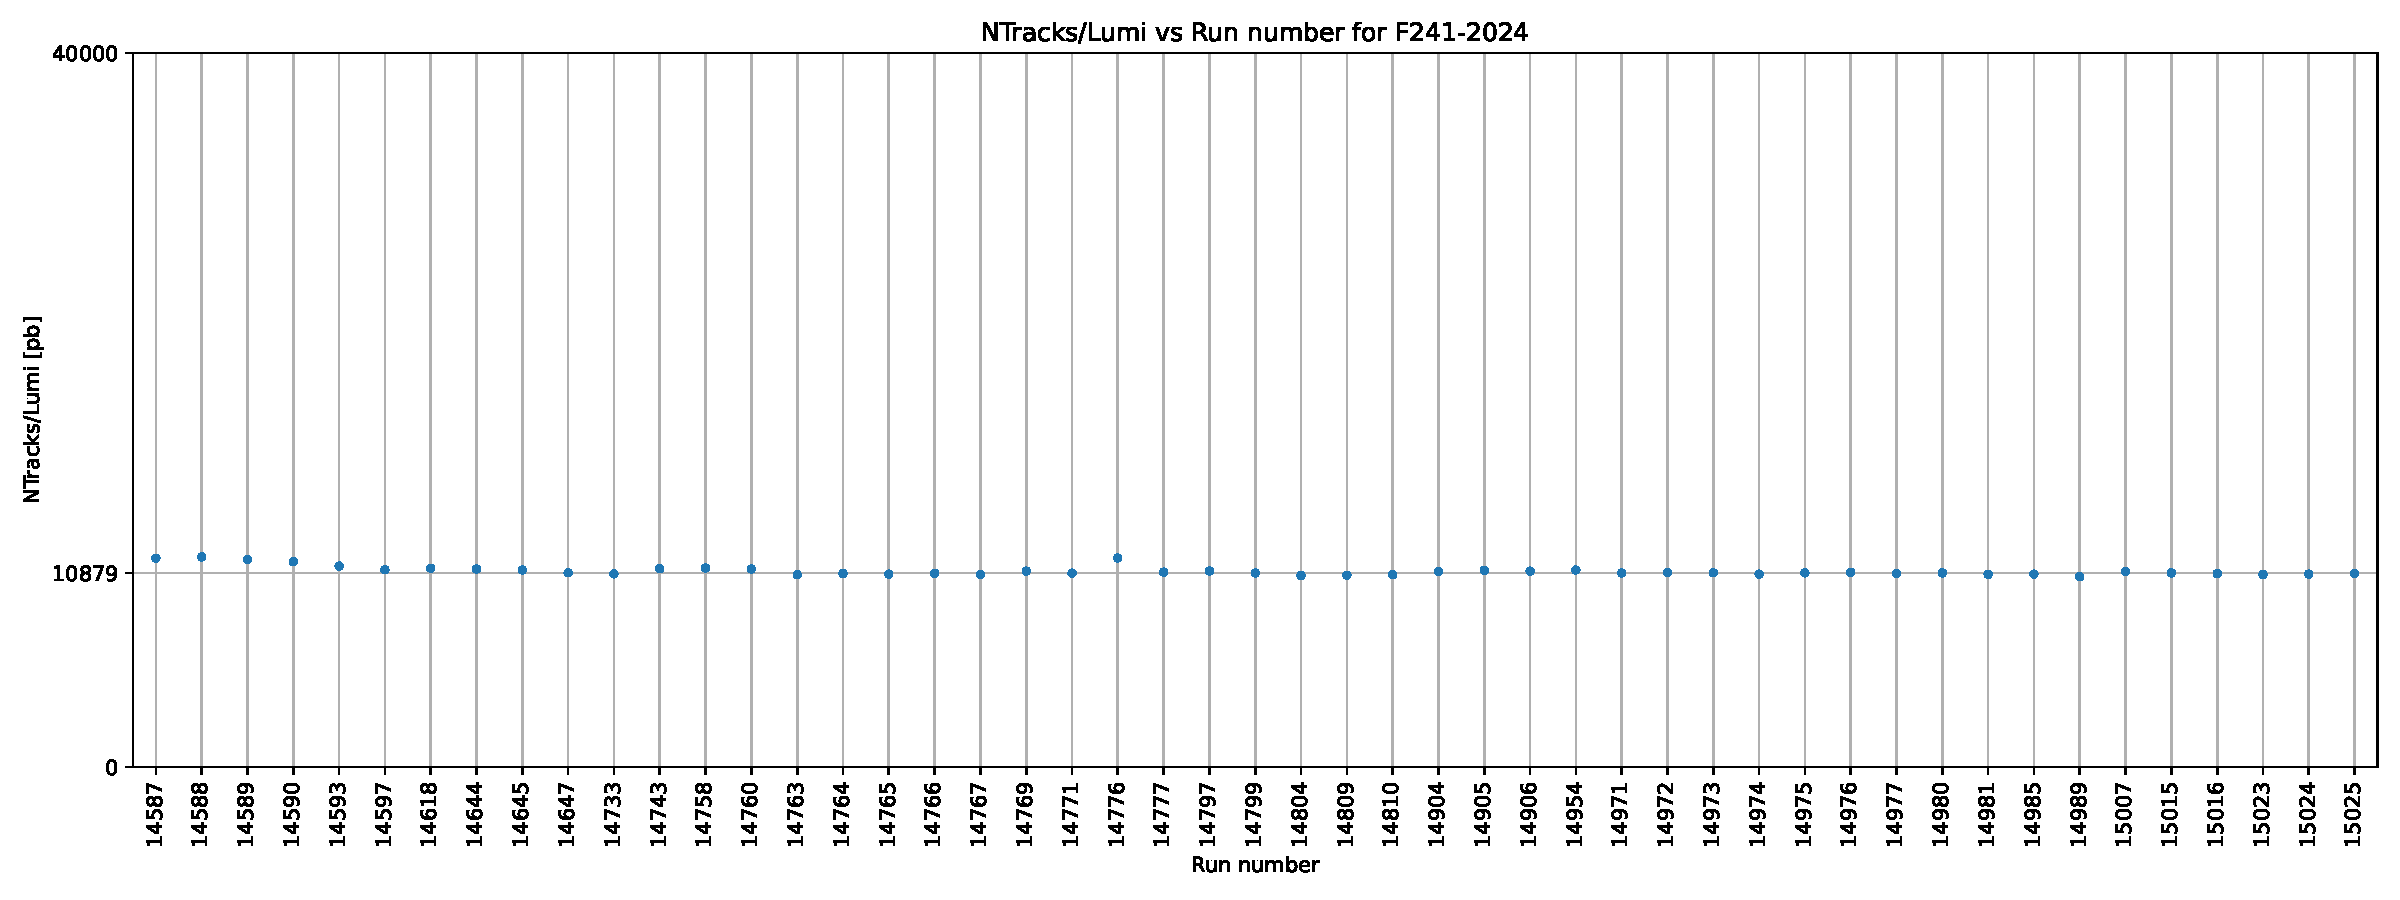
\includegraphics[height=0.4\textheight]{RunwisePlots/F241-2024_NTracksbyLumi.pdf}
% 	\end{figure}
% \end{frame}

% \begin{frame}{Yield Plots for Tungsten-2024}
% 	\begin{figure}
% 		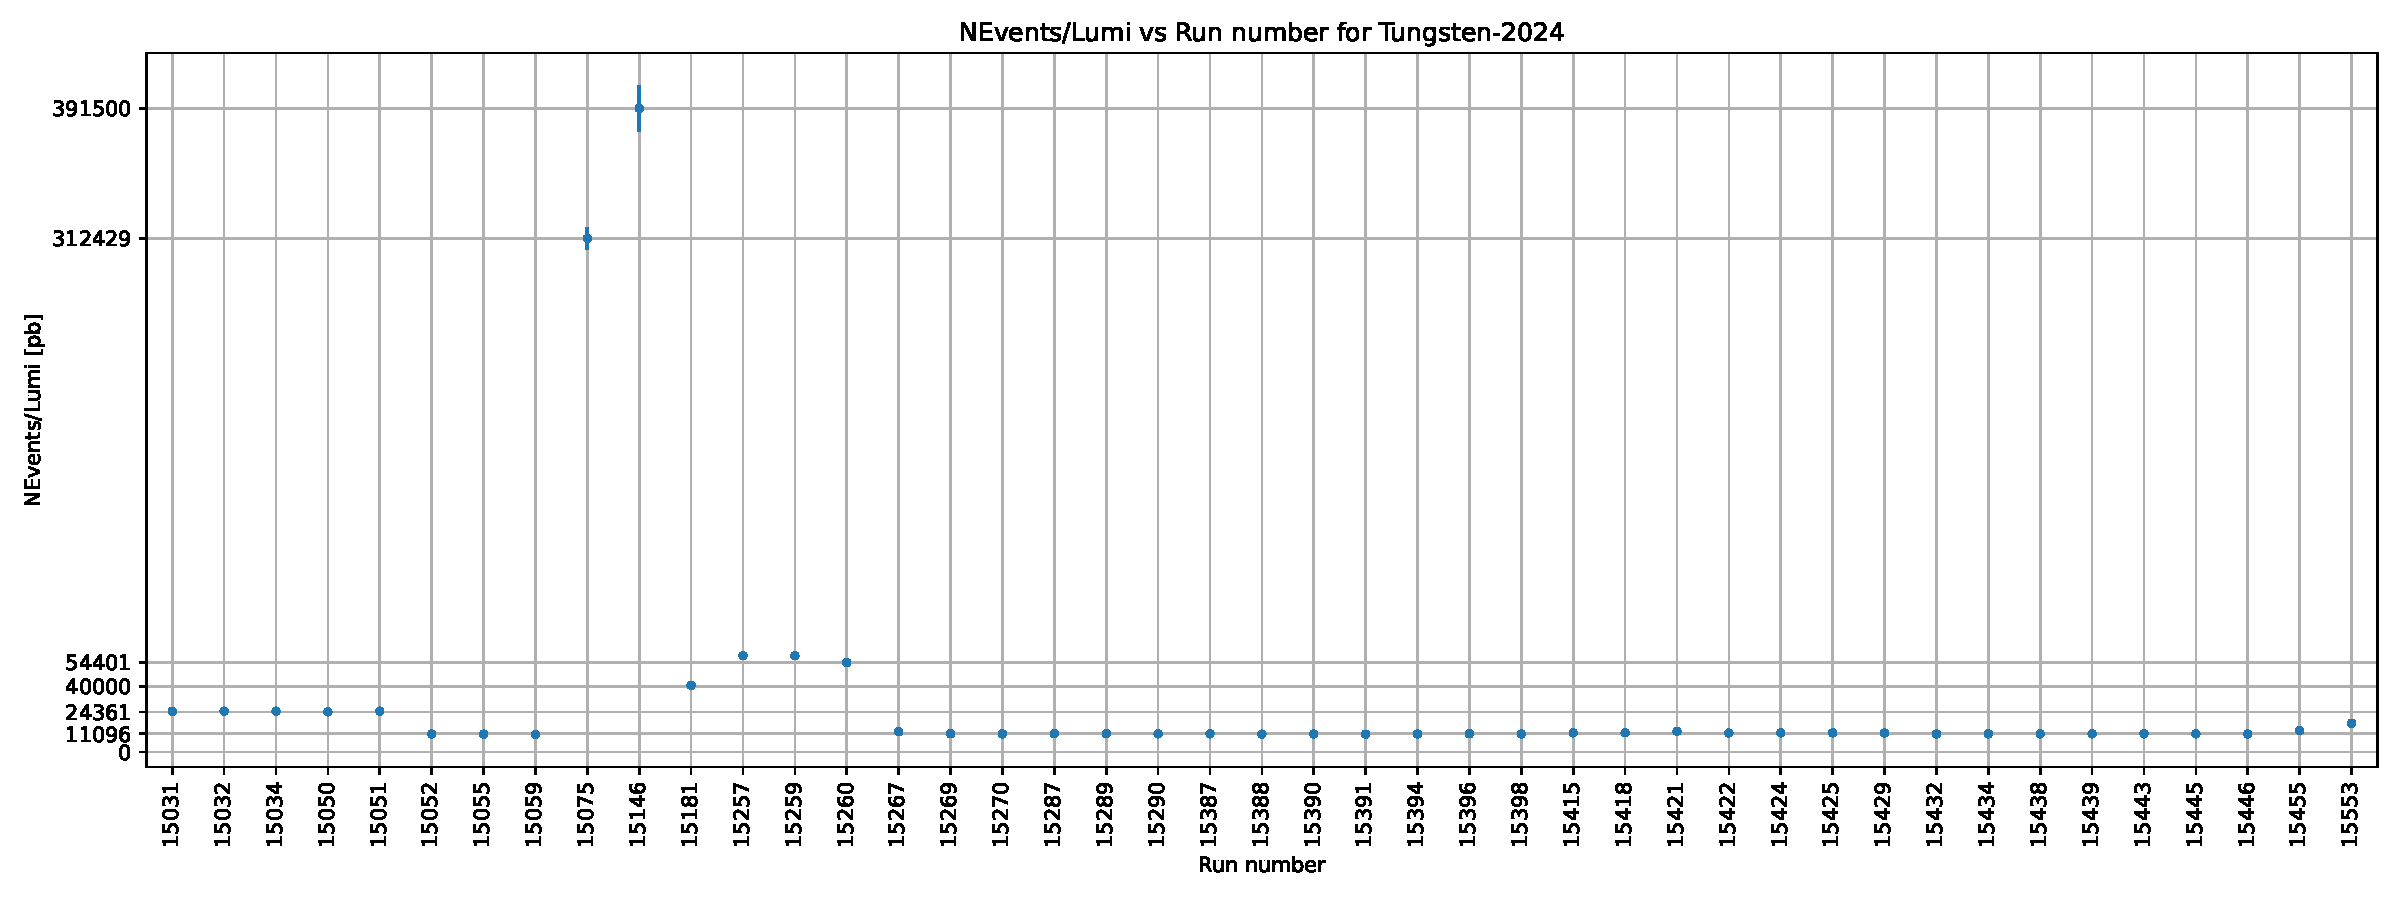
\includegraphics[height=0.4\textheight]{RunwisePlots/Tungsten-2024_NEventsbyLumi.pdf}
% 	\end{figure}
% 	\begin{figure}
% 		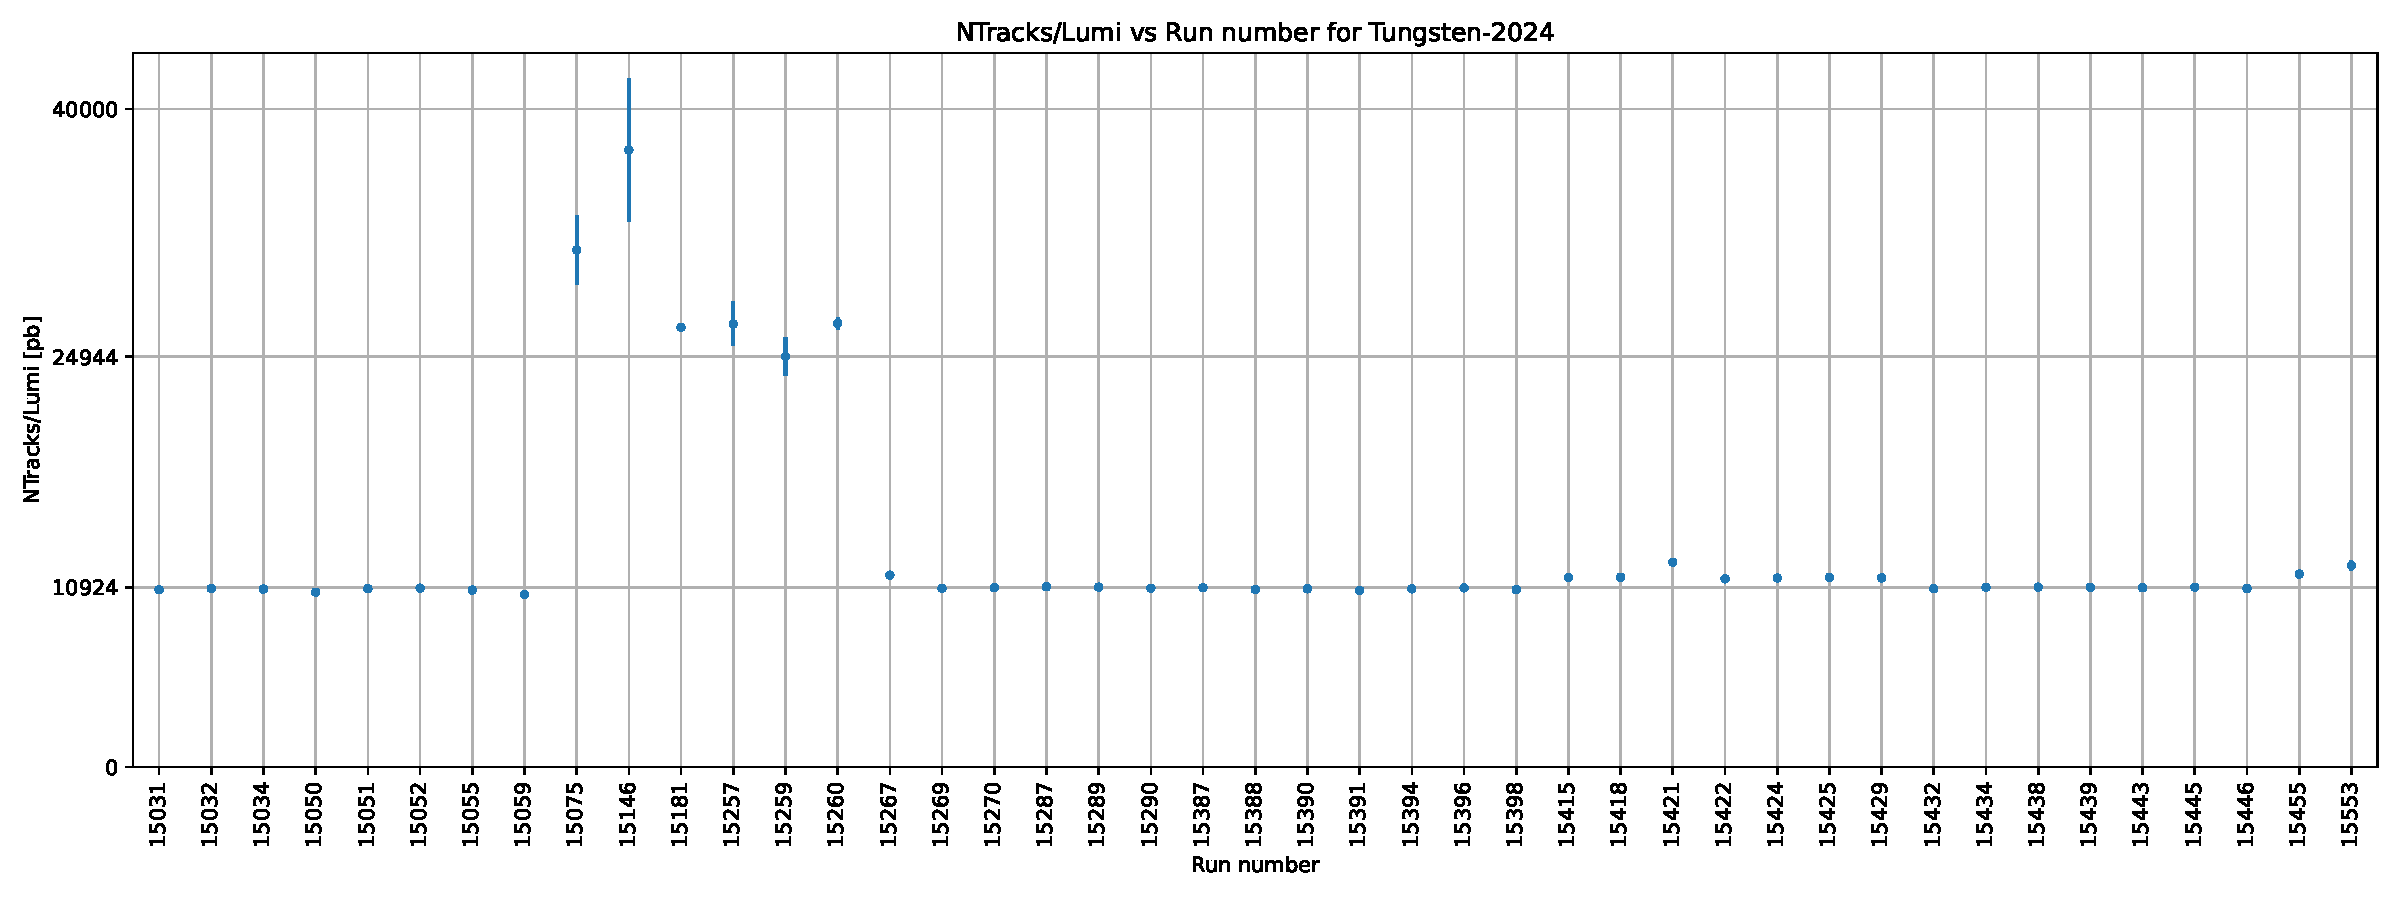
\includegraphics[height=0.4\textheight]{RunwisePlots/Tungsten-2024_NTracksbyLumi.pdf}
% 	\end{figure}
% \end{frame}

% \begin{frame}{Yield Plots for F242-2024}
% 	\begin{figure}
% 		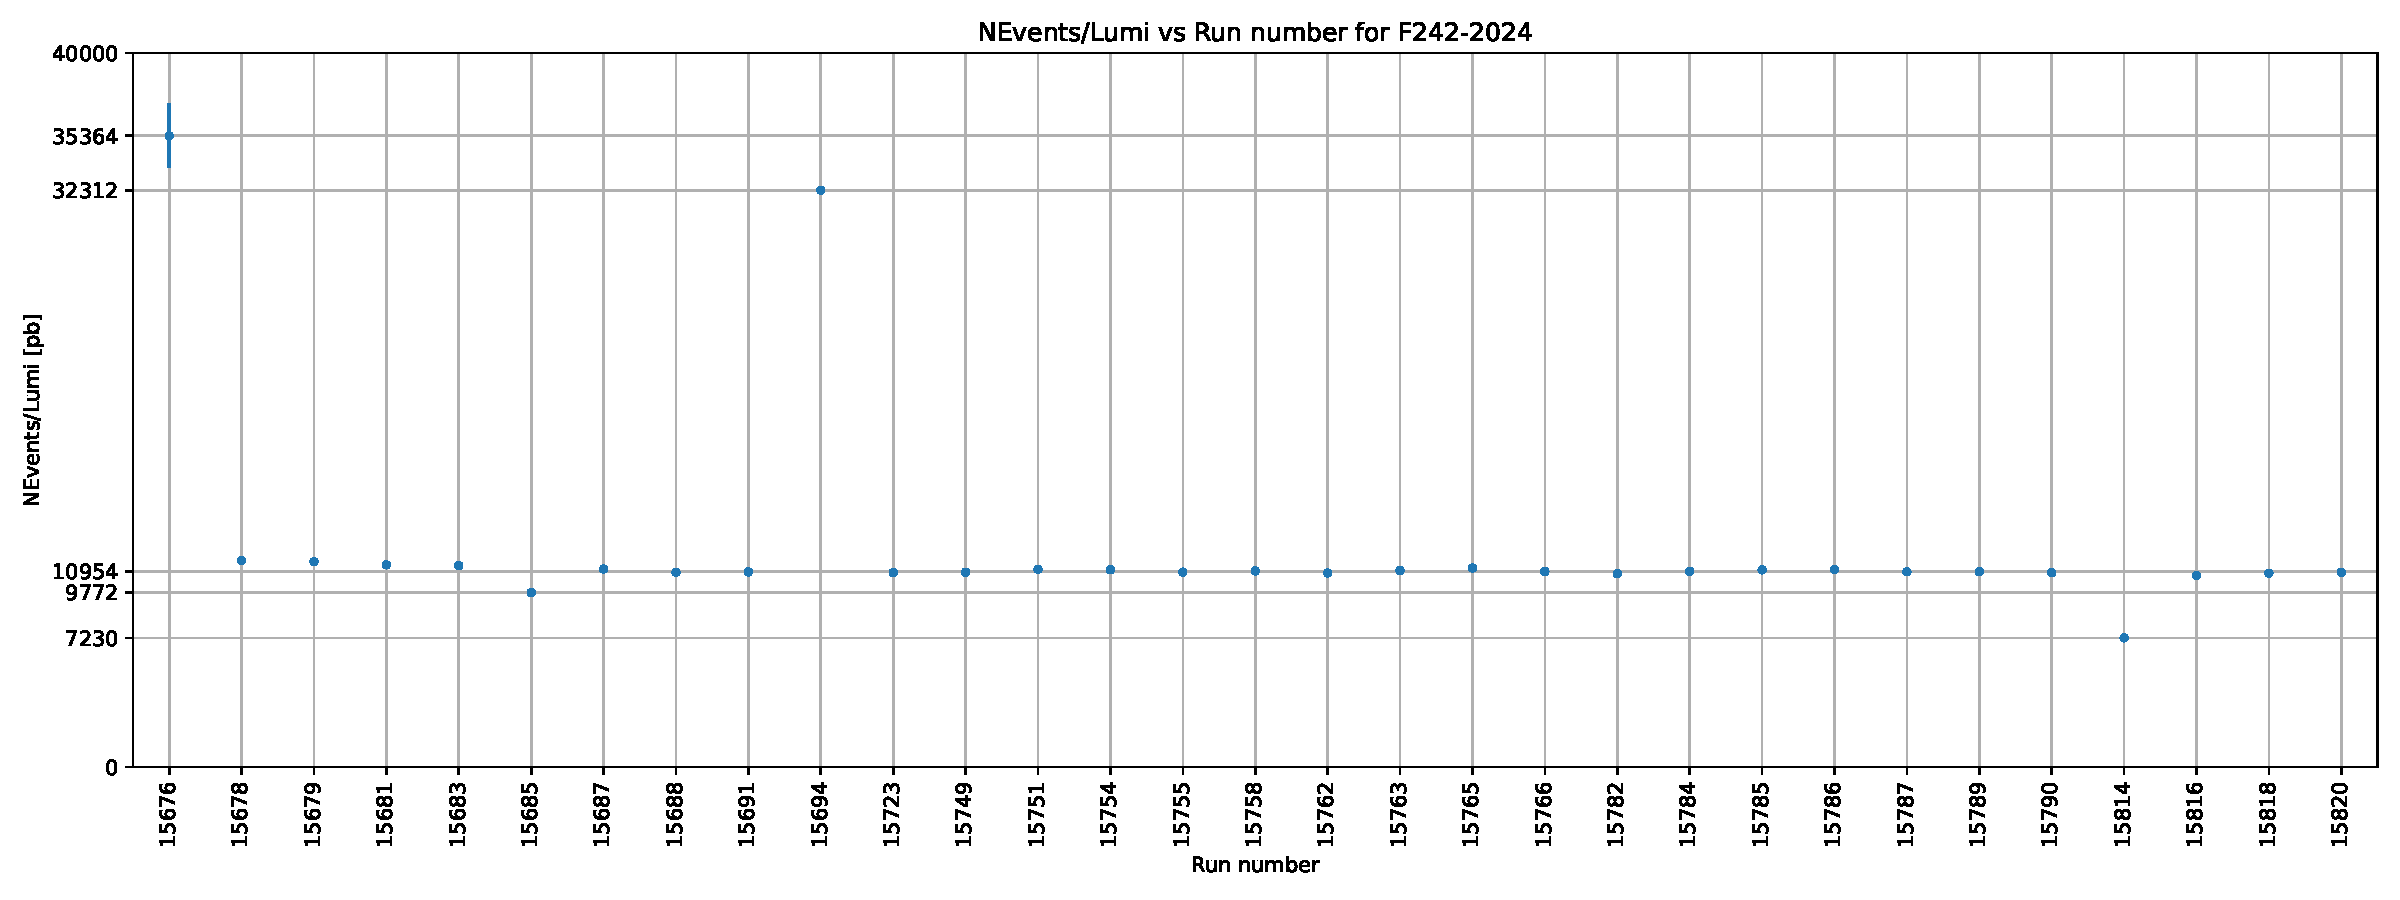
\includegraphics[height=0.4\textheight]{RunwisePlots/F242-2024_NEventsbyLumi.pdf}
% 	\end{figure}
% 	\begin{figure}
% 		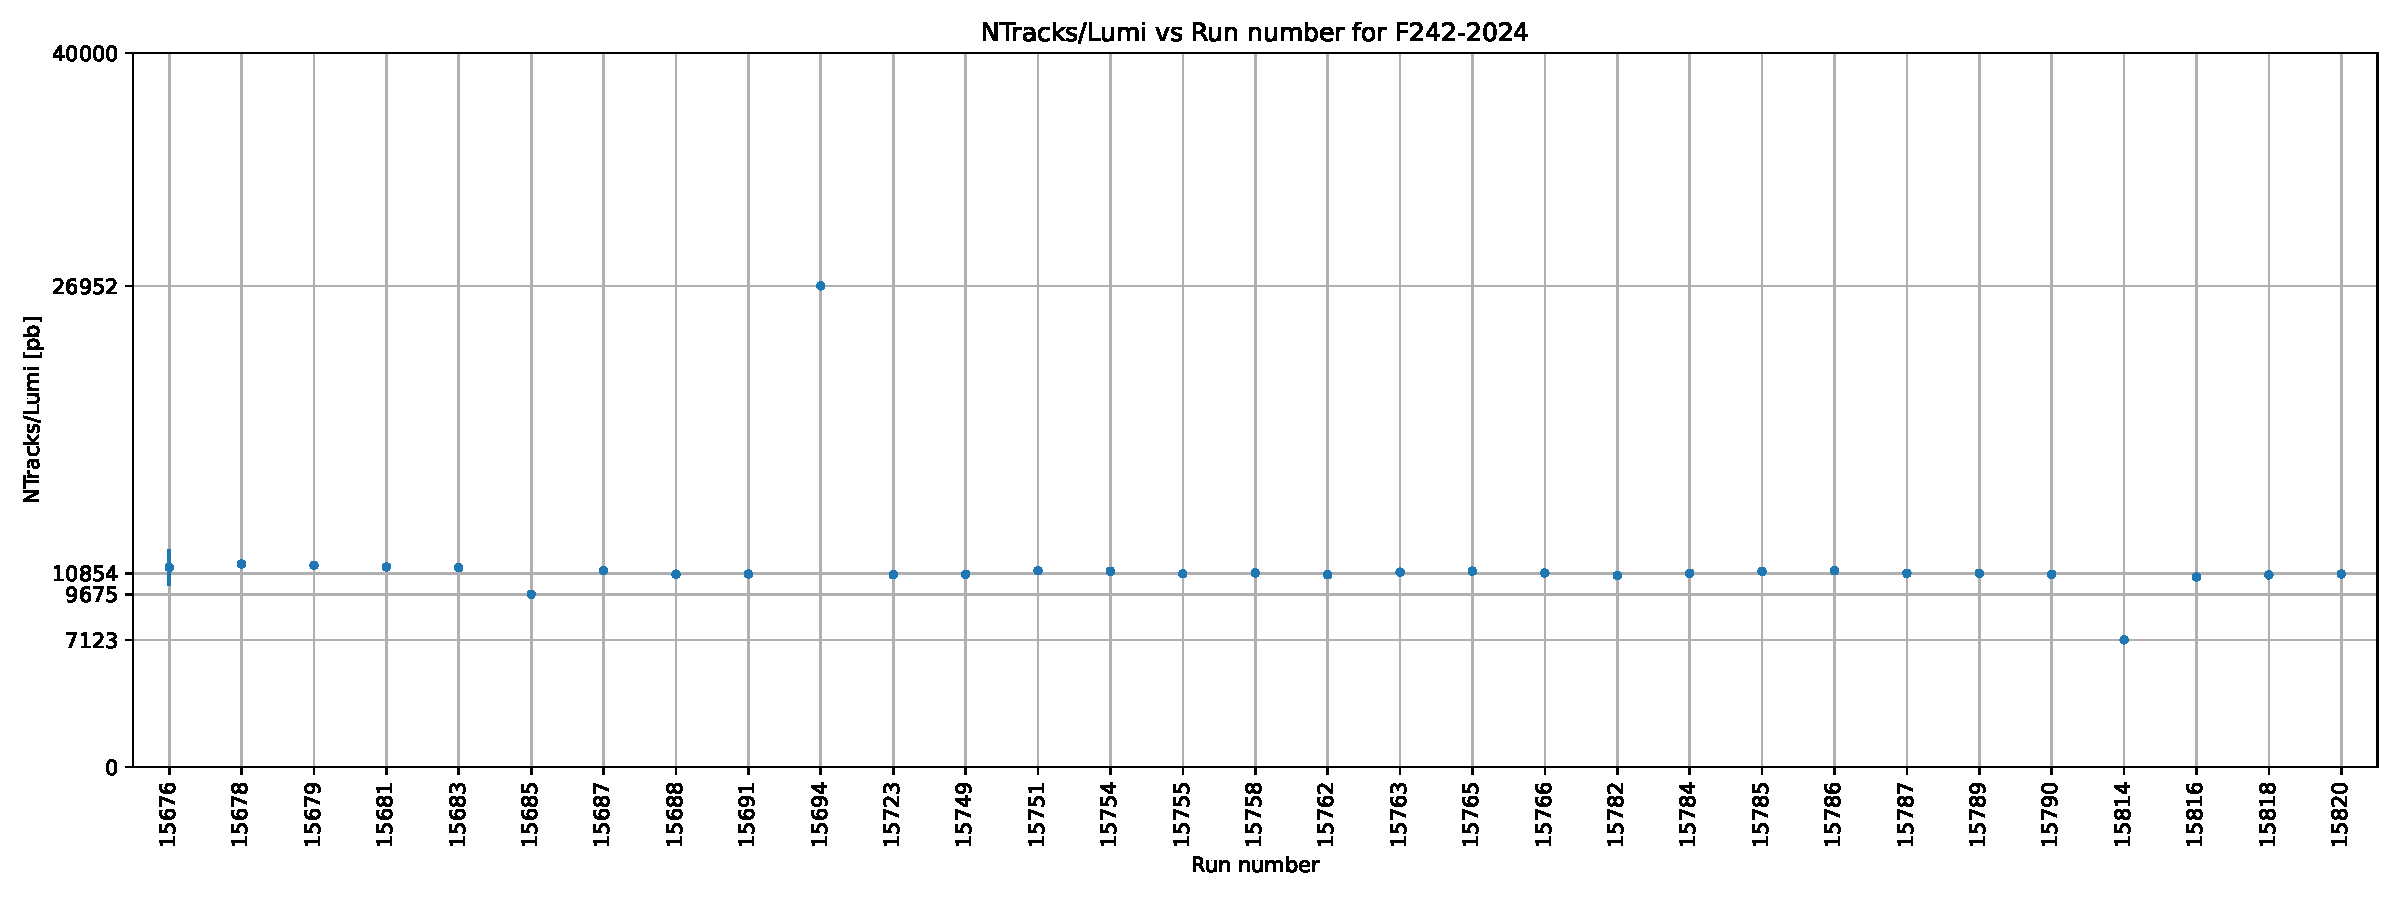
\includegraphics[height=0.4\textheight]{RunwisePlots/F242-2024_NTracksbyLumi.pdf}
% 	\end{figure}
% \end{frame}

% \begin{frame}{Yield Plots for CaloNu-2024}
% 	\begin{figure}
% 		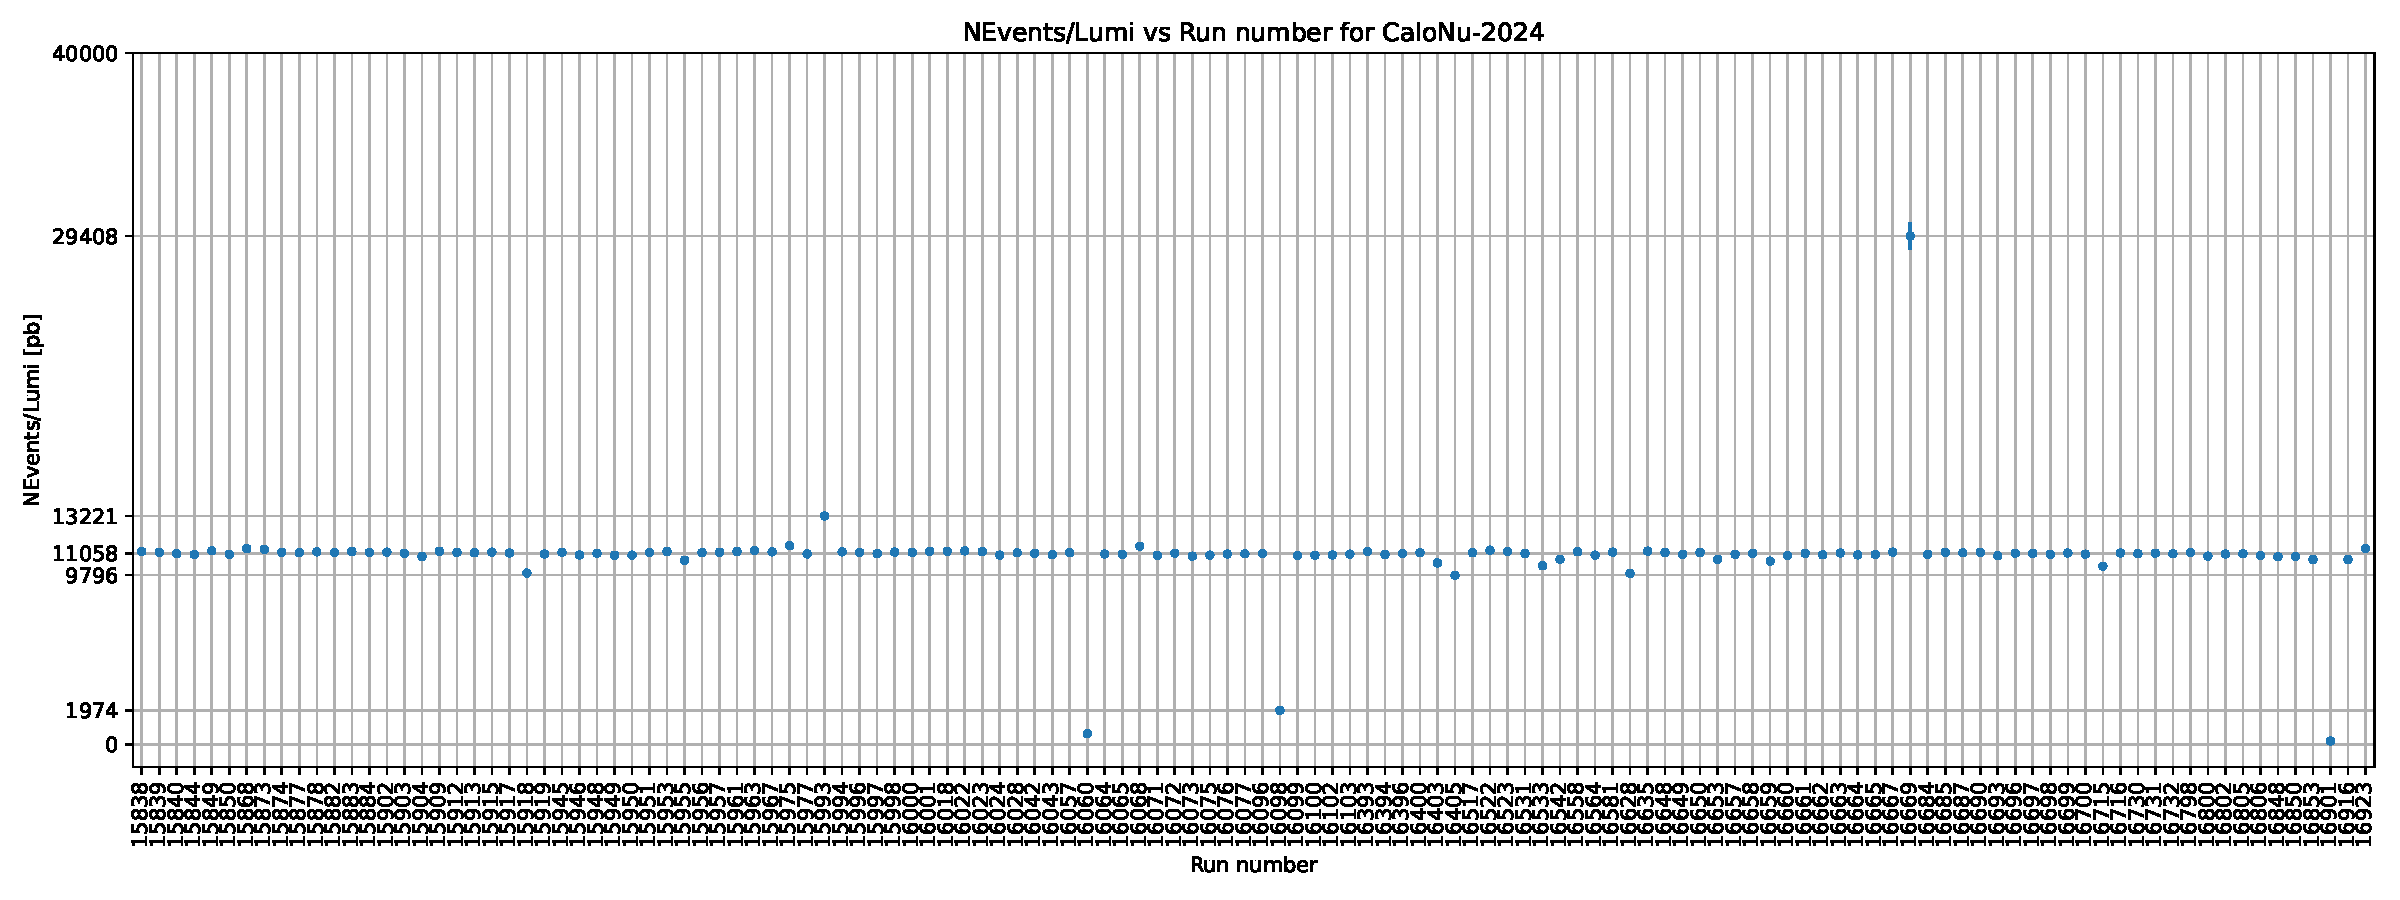
\includegraphics[height=0.4\textheight]{RunwisePlots/CaloNu-2024_NEventsbyLumi.pdf}
% 	\end{figure}
% 	\begin{figure}
% 		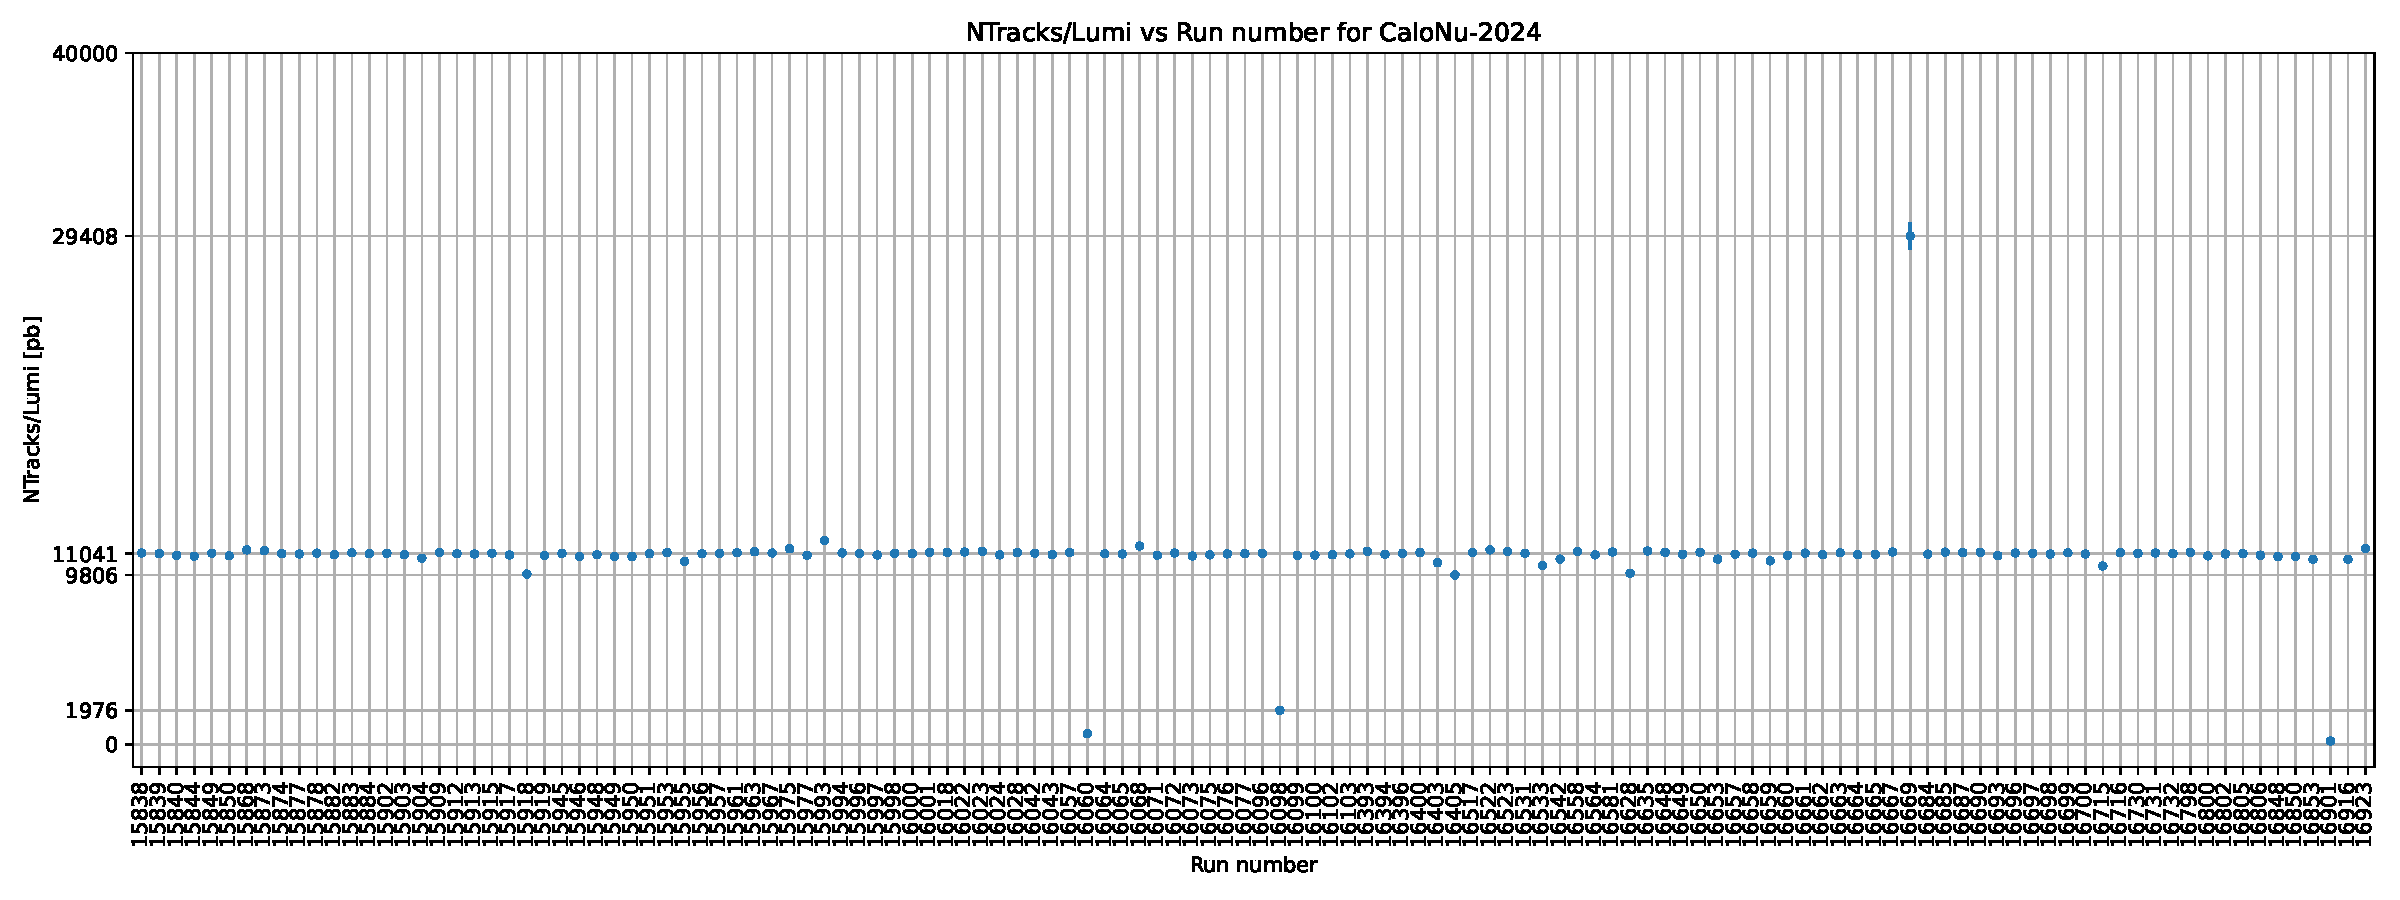
\includegraphics[height=0.4\textheight]{RunwisePlots/CaloNu-2024_NTracksbyLumi.pdf}
% 	\end{figure}
% \end{frame}

% \begin{frame}{Yield Plots for F243-2024}
% 	\begin{figure}
% 		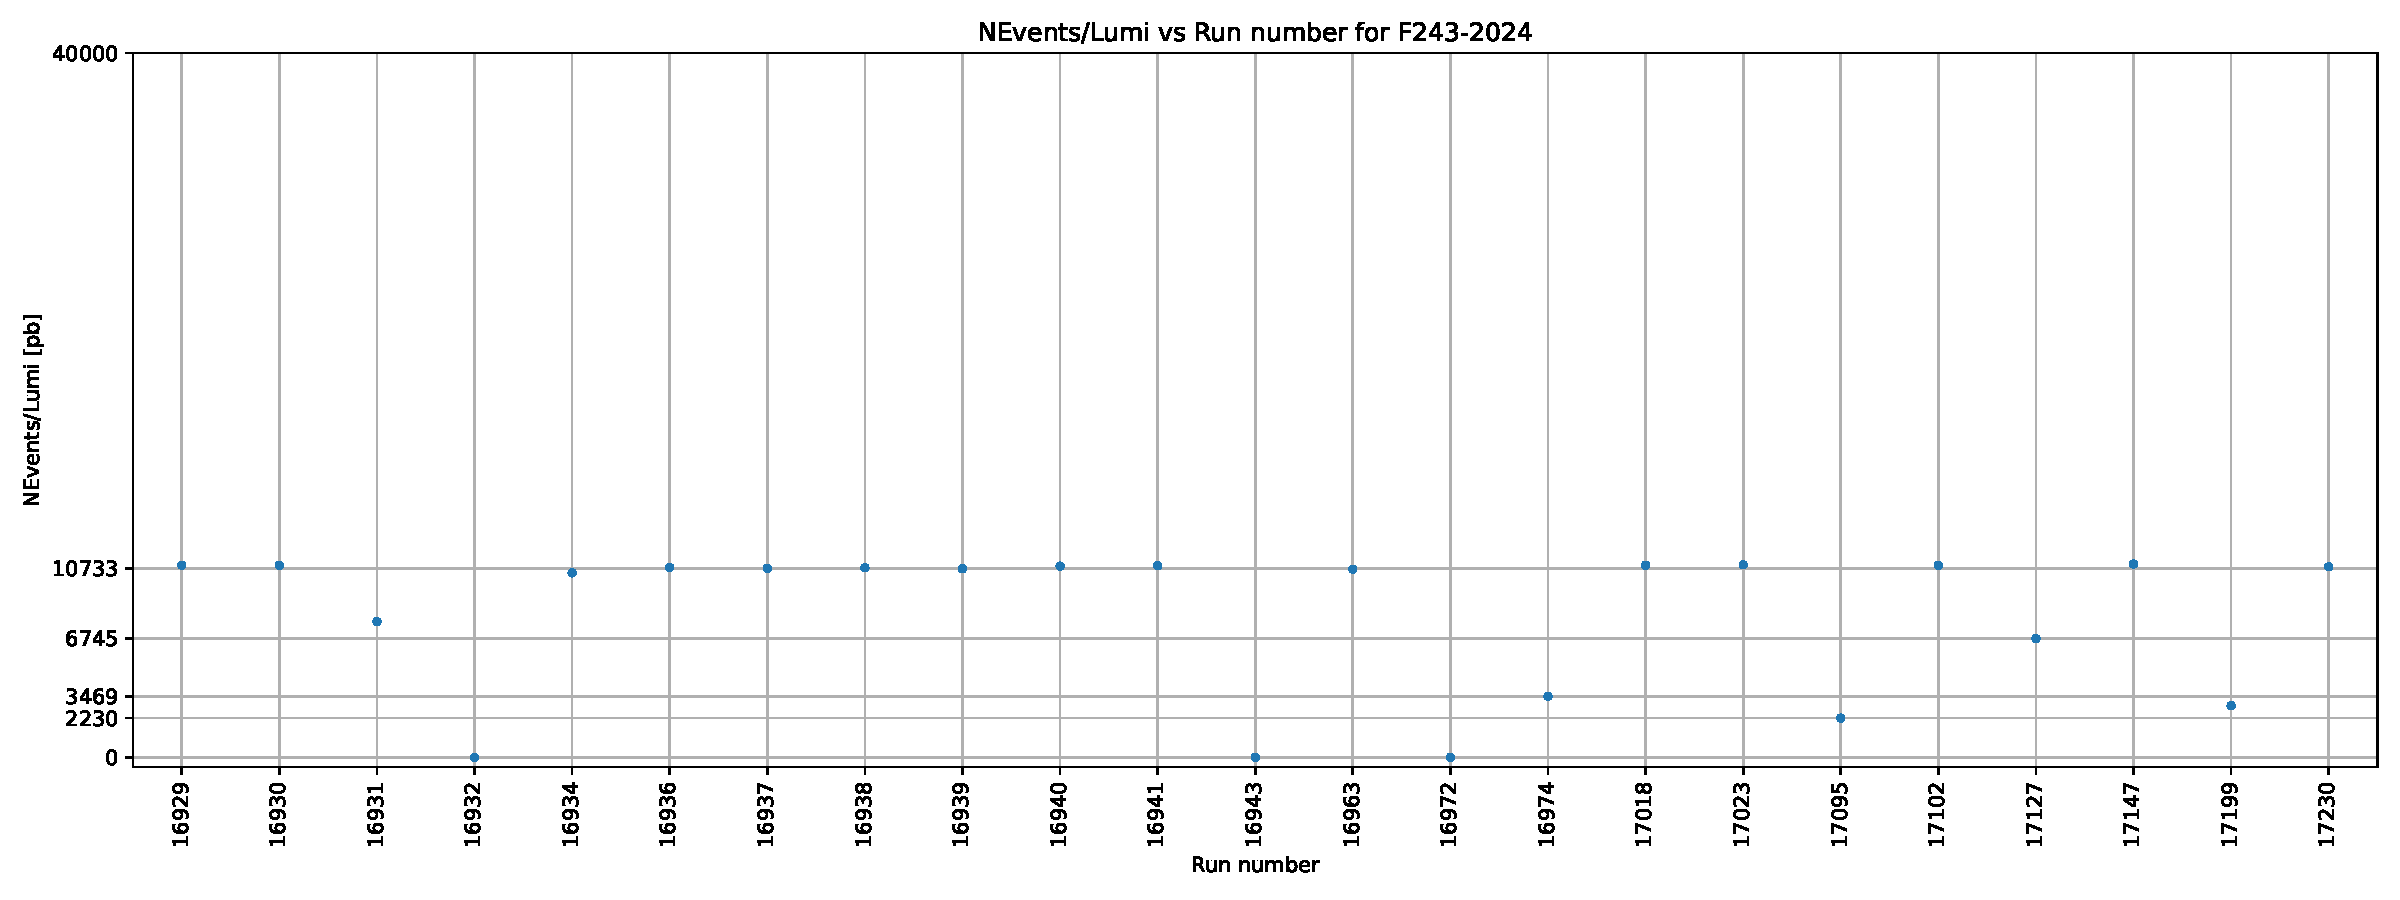
\includegraphics[height=0.4\textheight]{RunwisePlots/F243-2024_NEventsbyLumi.pdf}
% 	\end{figure}
% 	\begin{figure}
% 		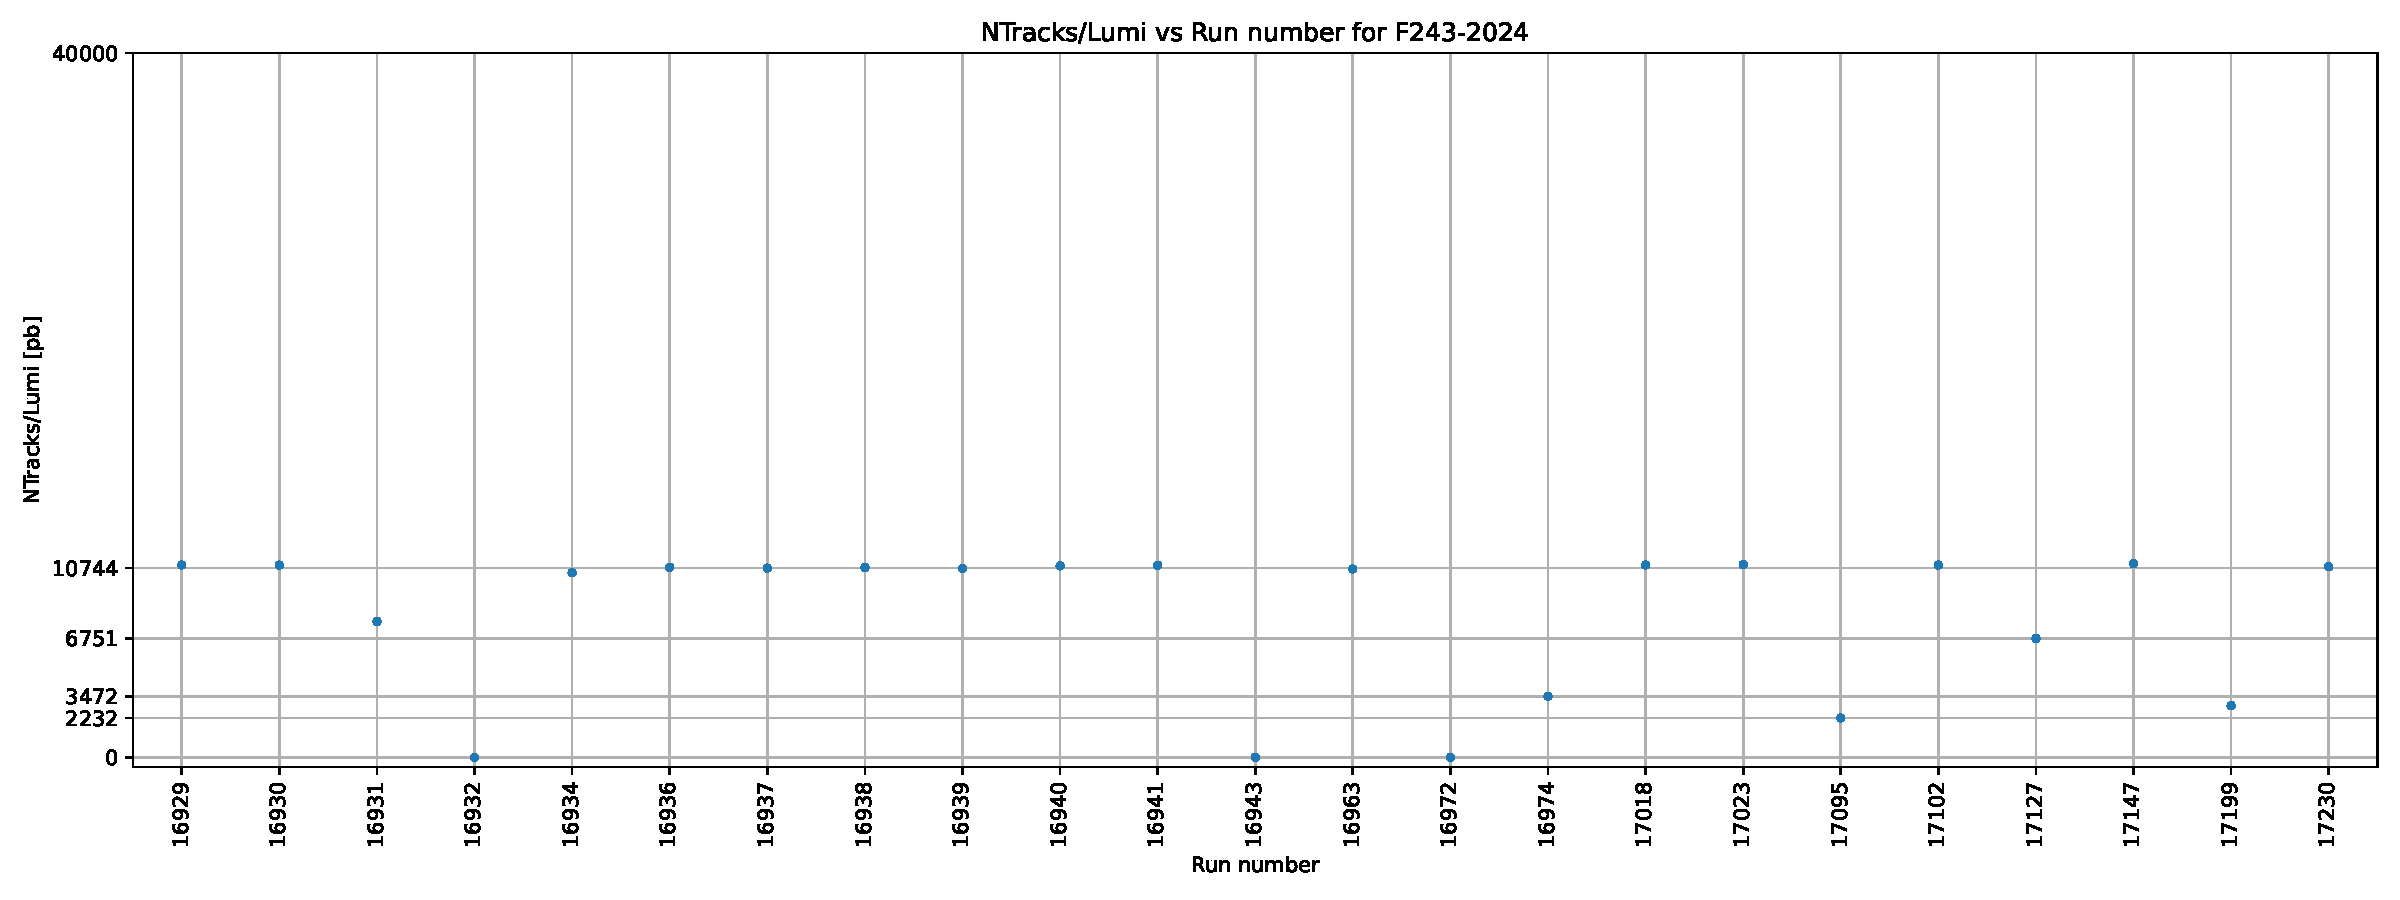
\includegraphics[height=0.4\textheight]{RunwisePlots/F243-2024_NTracksbyLumi.pdf}
% 	\end{figure}
% \end{frame}

\begin{frame}{Median Yields across Runs}
	\begin{figure}
		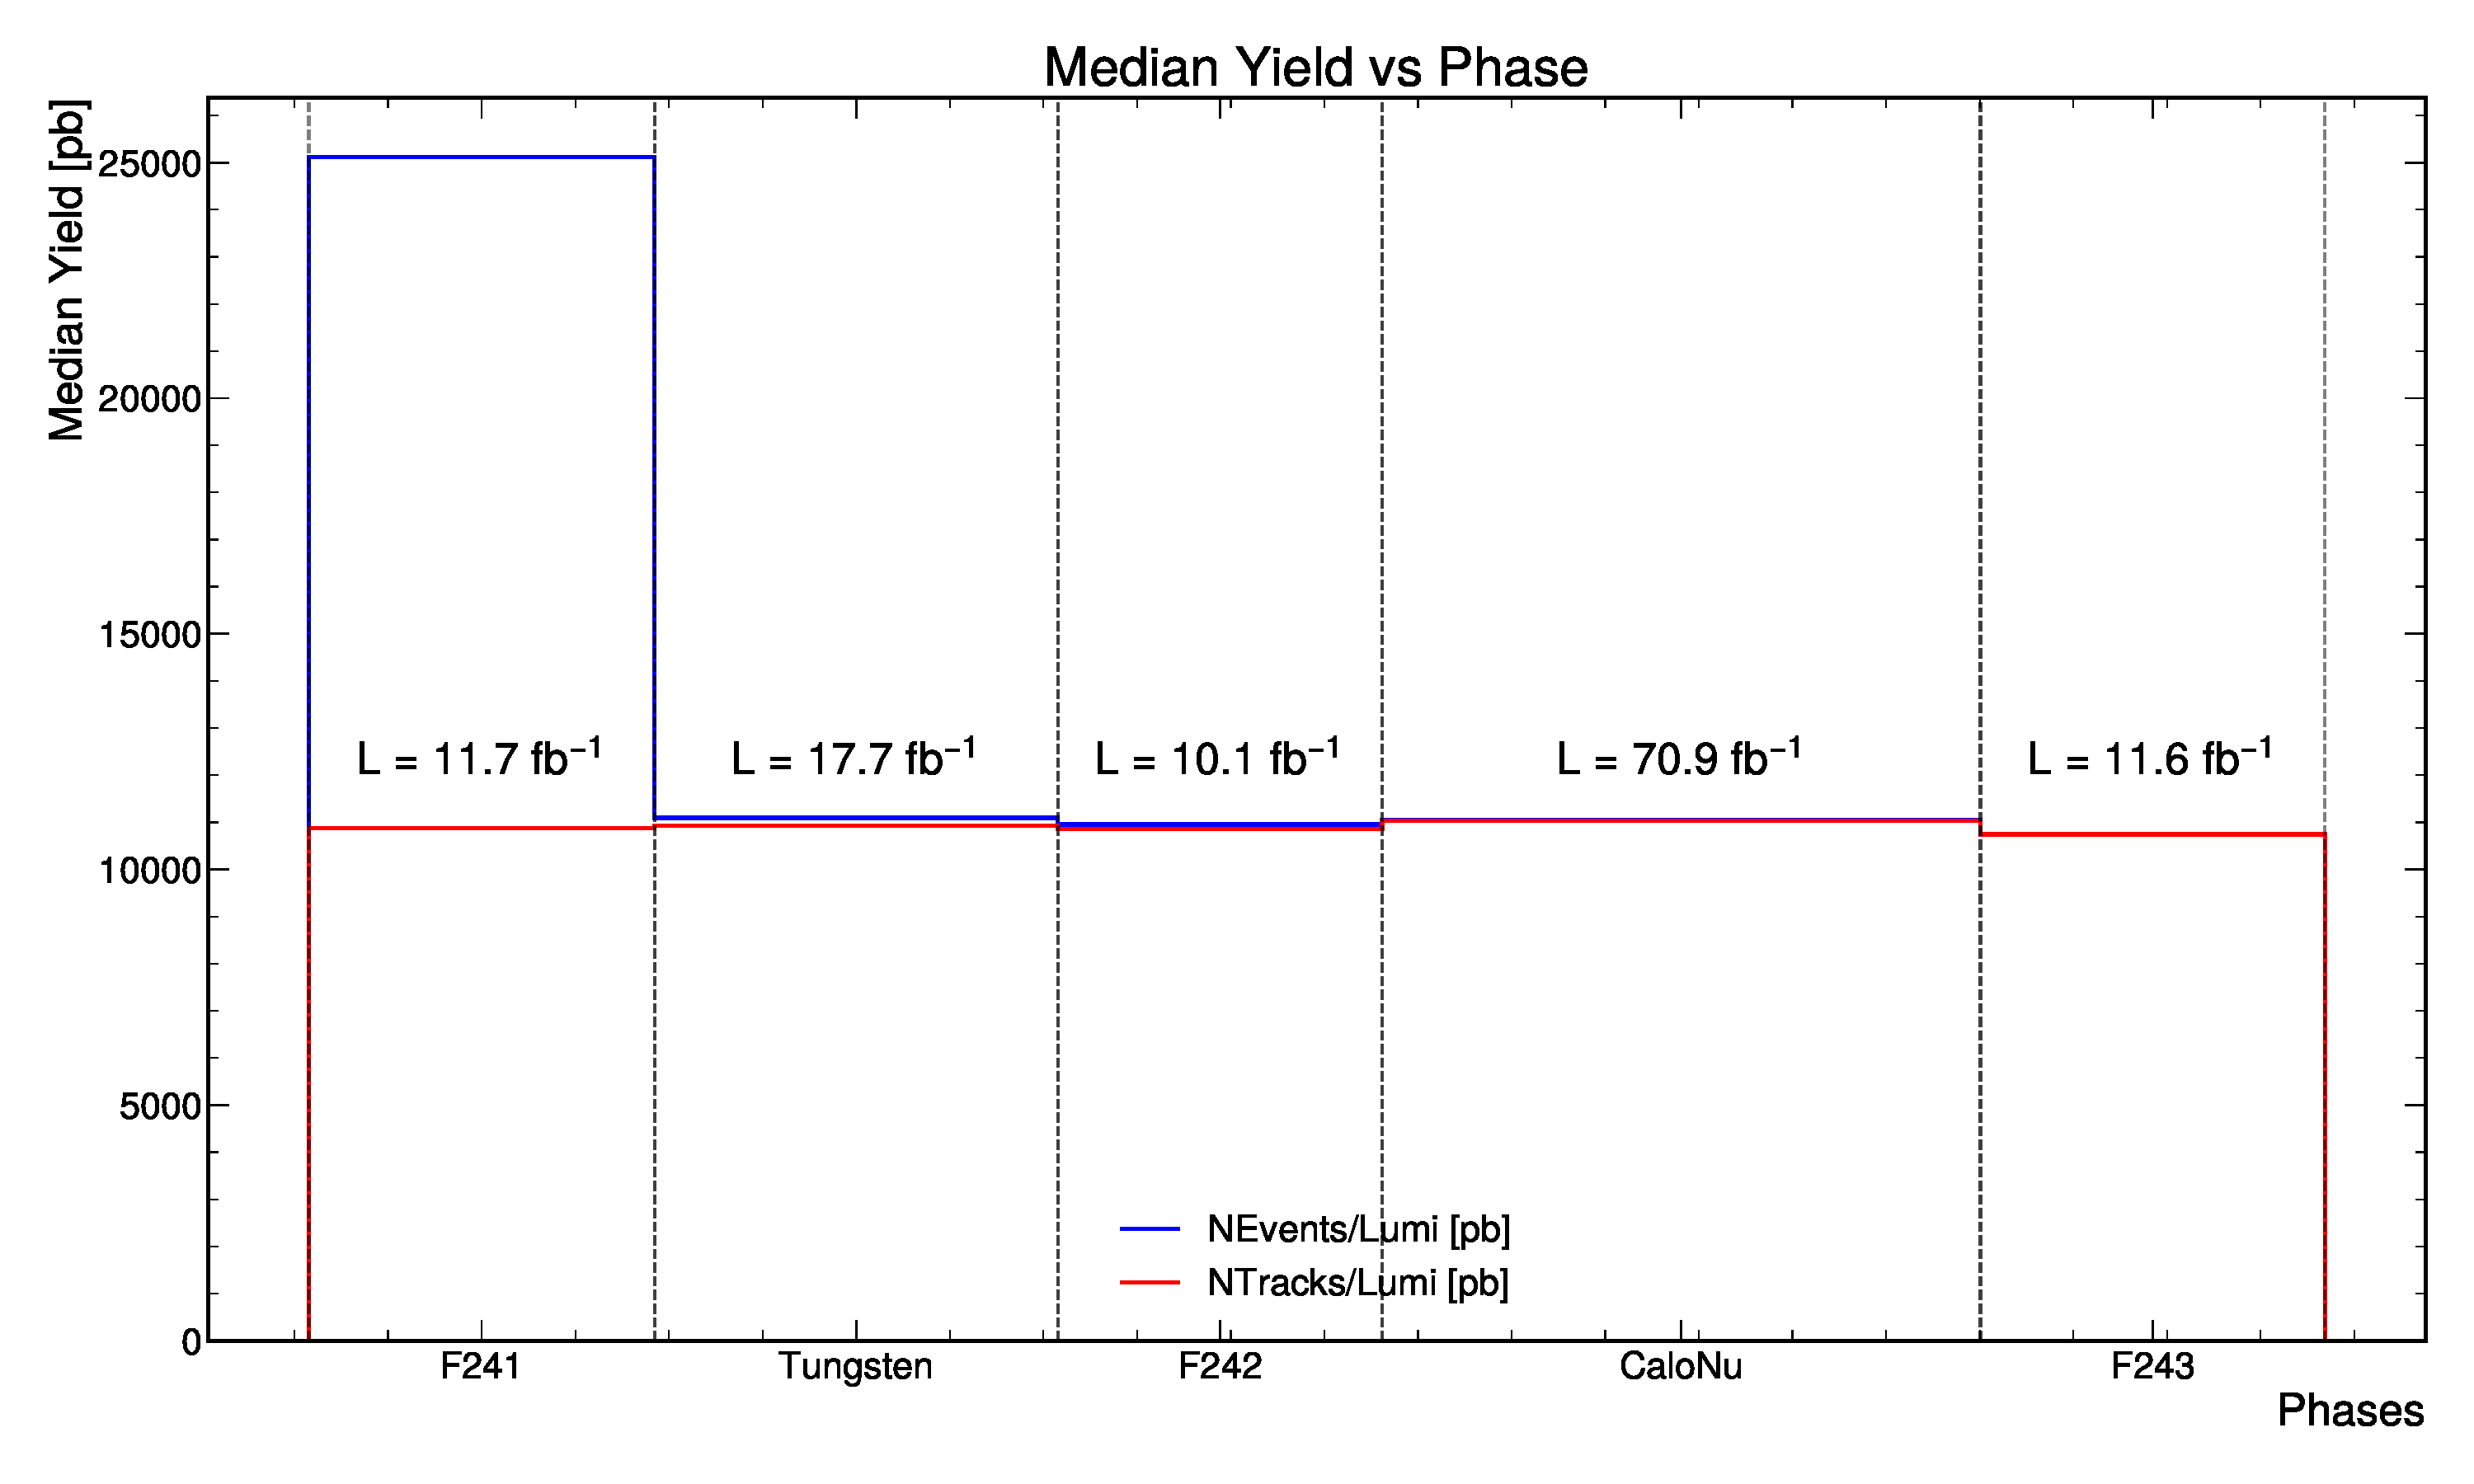
\includegraphics[width=\linewidth]{./RunwisePlots/MedianYieldsPhase.pdf}
	\end{figure}
	\vspace{-0.5cm}
	\begin{itemize}
		\item Possible anomaly in the F241 data from lack of BCID cut.
		\item Detailed Listing of runs with problematic yields. \href{https://docs.google.com/spreadsheets/d/1nnYFcmhVieSHI5XAVhPiW1K6CoGYGxv2YPchwL0sqH4/edit?usp=sharing}{[LINK]}
	\end{itemize}
\end{frame}

% \begin{frame}{Distribution of Track Parameters across Runs}
% 	\begin{center}
% 		Excellent agreement of variables across runs !
% 	\end{center}
	
% \end{frame}


\begin{frame}{Distribution of Track Position/Angle across runs}
	\begin{columns}
		\begin{column}{0.5\linewidth}
			\vspace{-0.4cm}
			\begin{figure}
				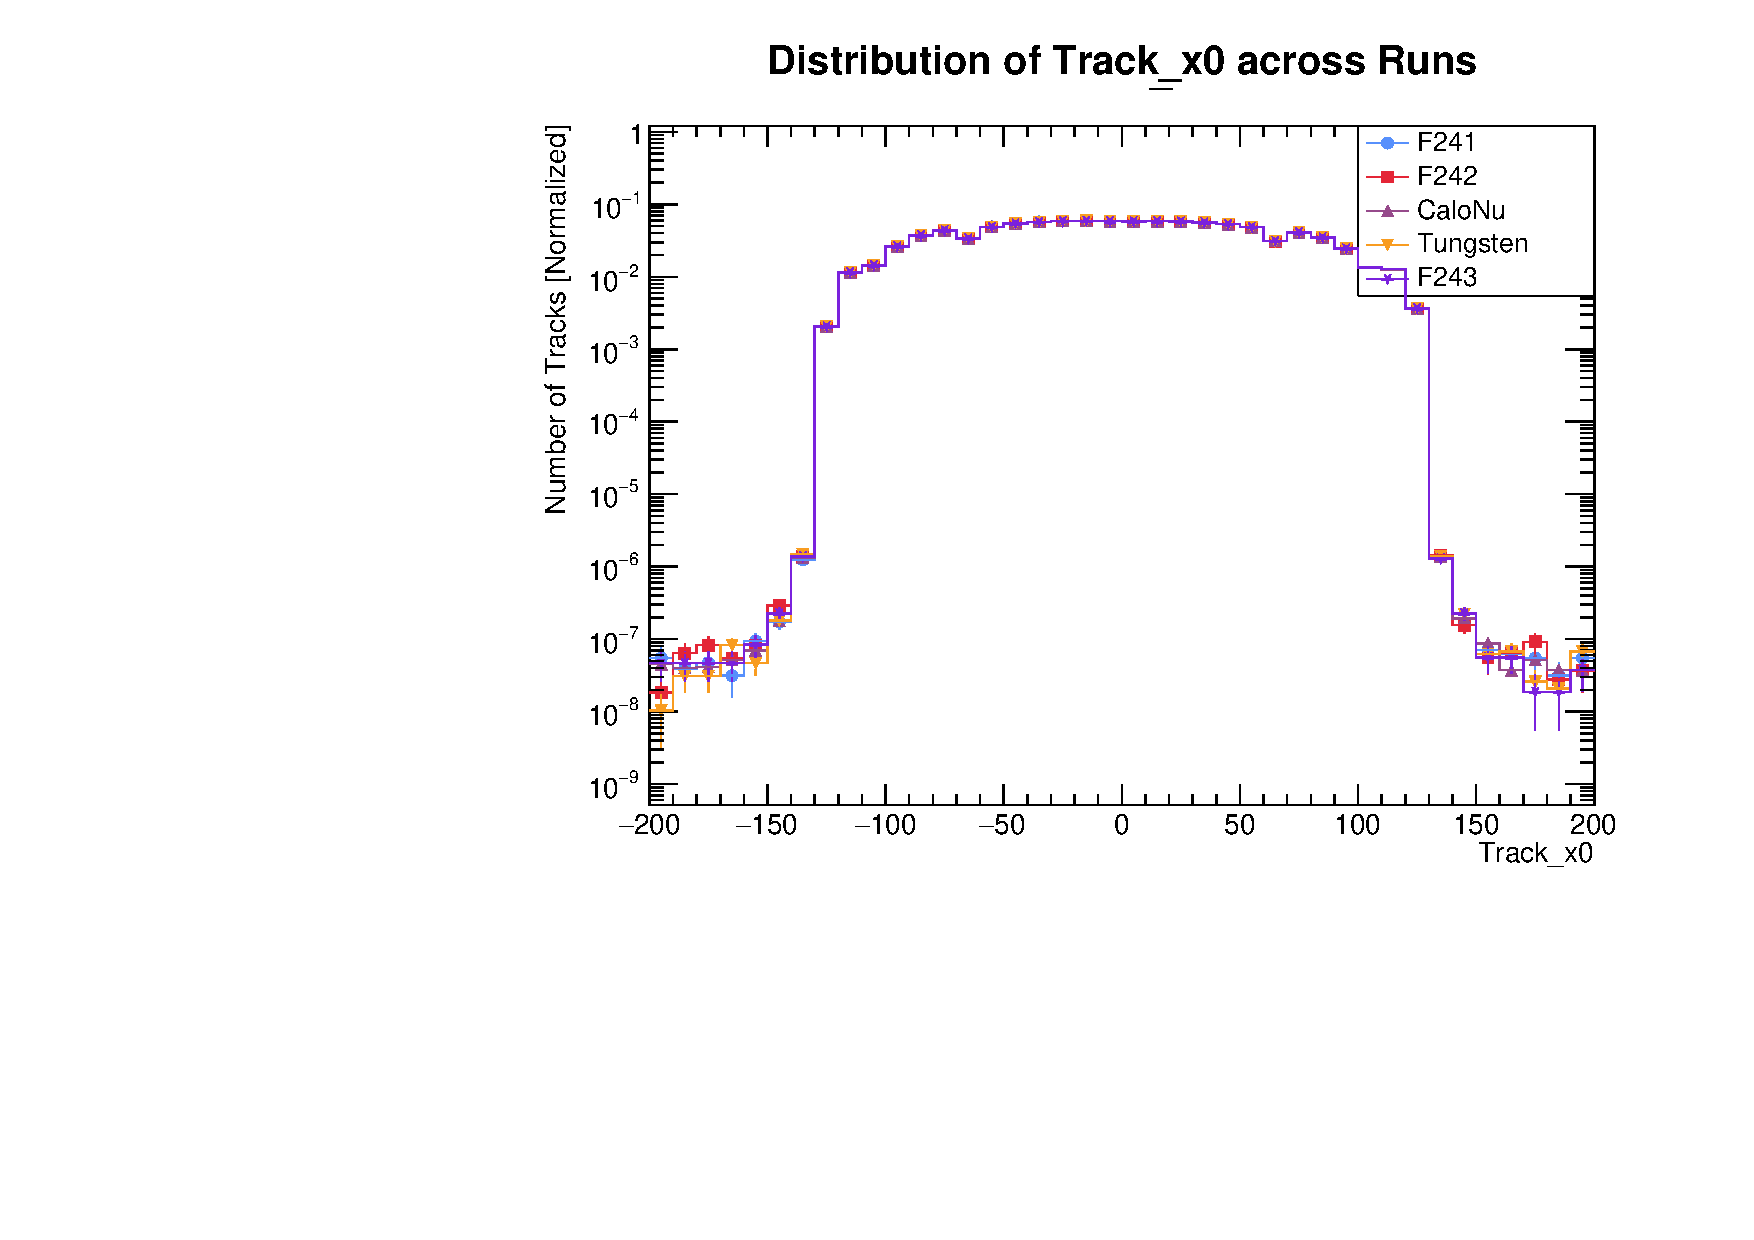
\includegraphics[width=\linewidth]{./RunwisePlots/Track_x0_runwise.pdf}
				\caption{Distribution of Track Position X0}
			\end{figure}
			\vspace{-0.9cm}
			\begin{figure}
				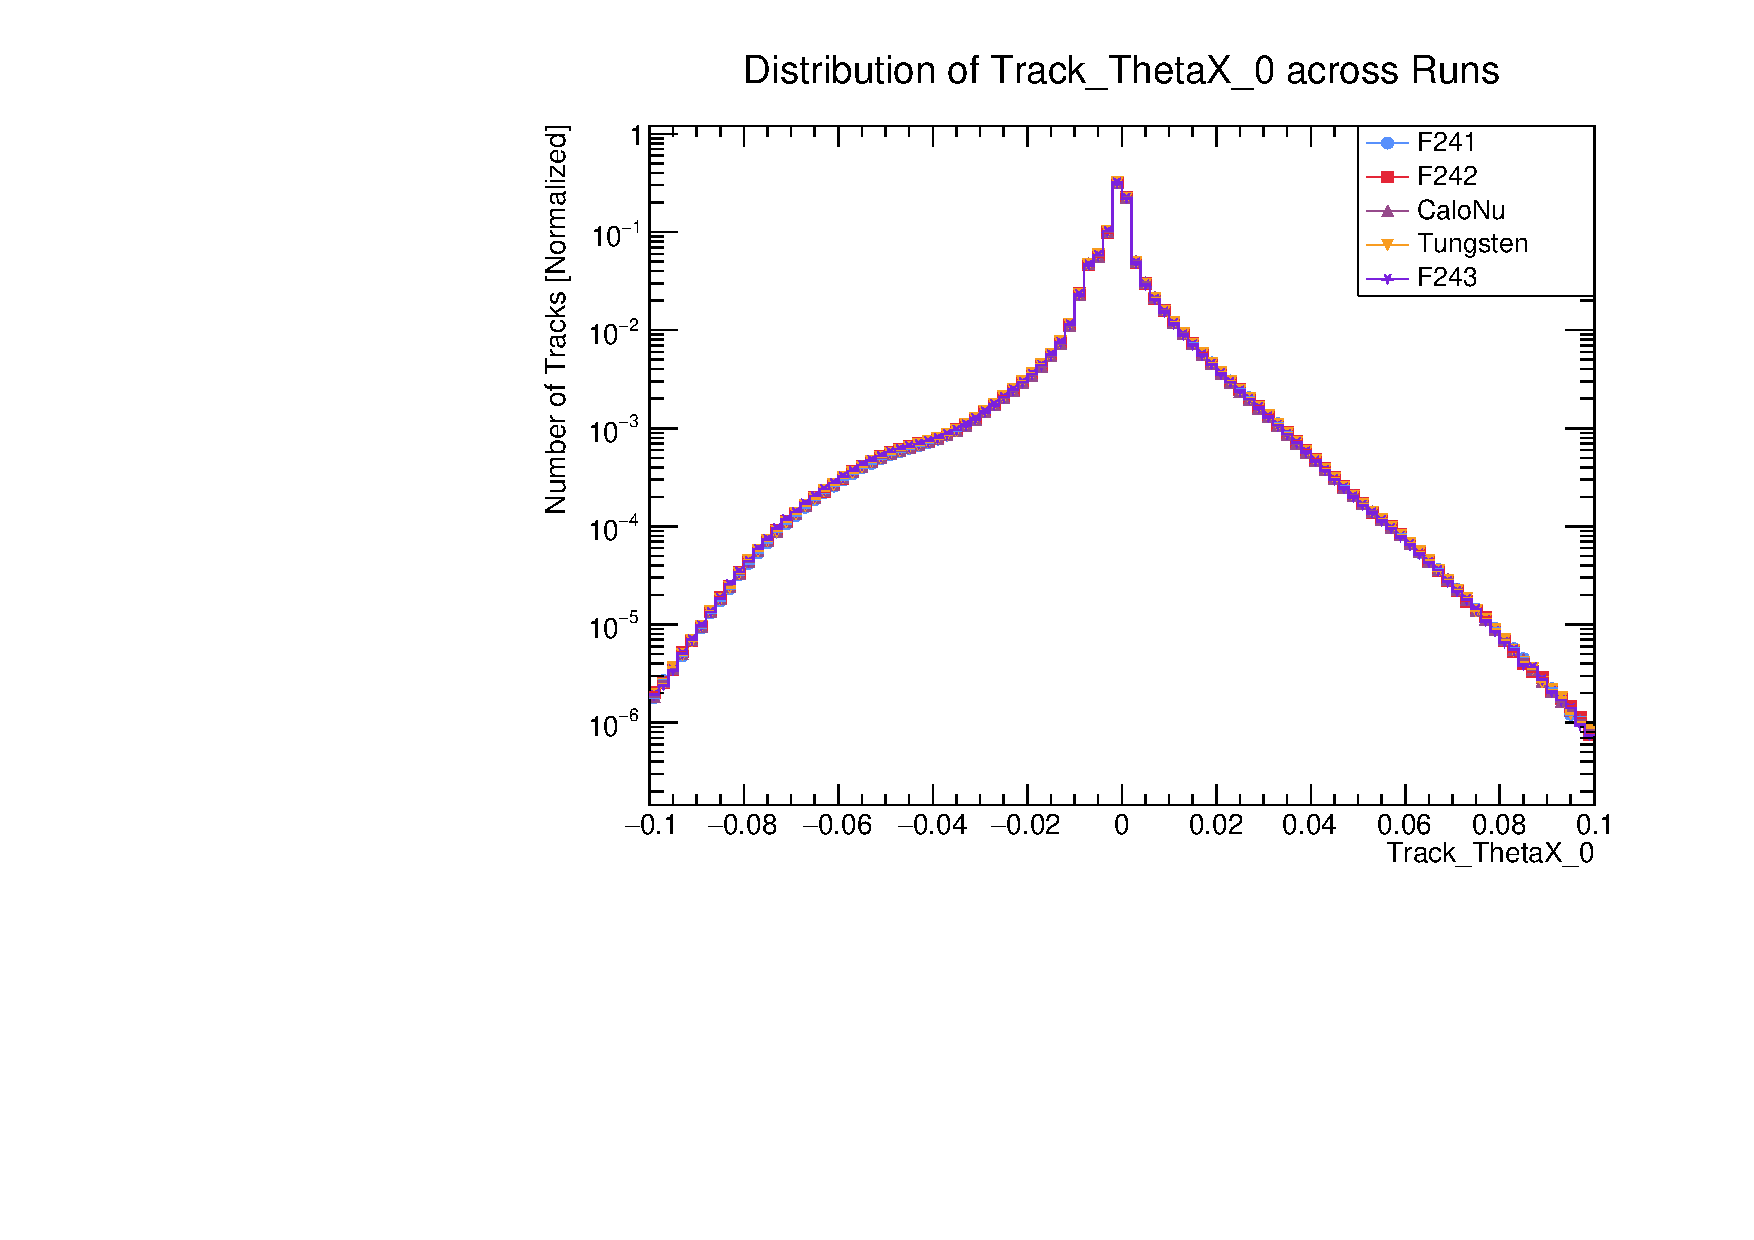
\includegraphics[width=\linewidth]{./RunwisePlots/Track_ThetaX_0_runwise.pdf}
				\caption{Distribution of Track ThetaX0 across 2024 runs}
			\end{figure}
		\end{column}
		\begin{column}{0.5 \linewidth}
			\vspace{-0.4cm}
			\begin{figure}
				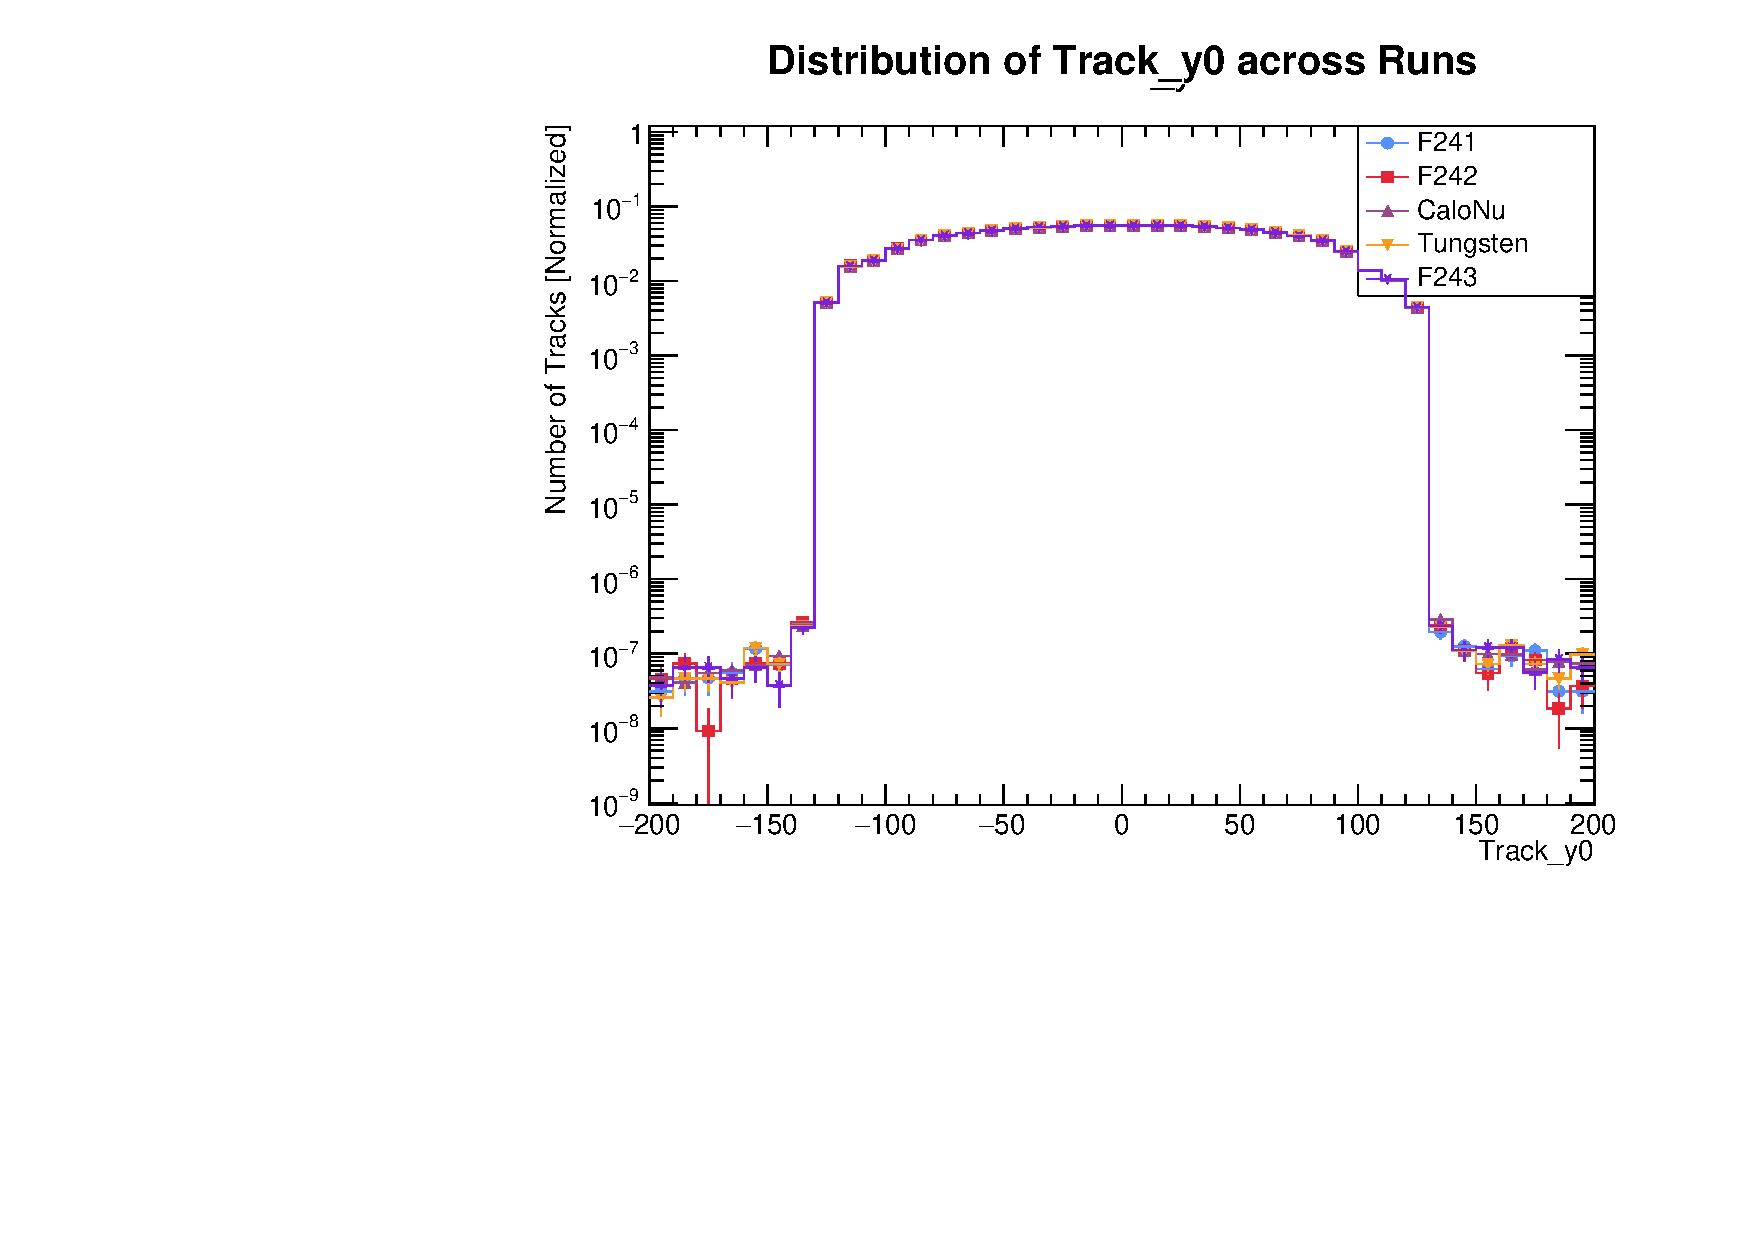
\includegraphics[width=\linewidth]{./RunwisePlots/Track_y0_runwise.pdf}
				\caption{Distribution of Track Position in Y0}
			\end{figure}
			\vspace{-0.9cm}
			\begin{figure}
				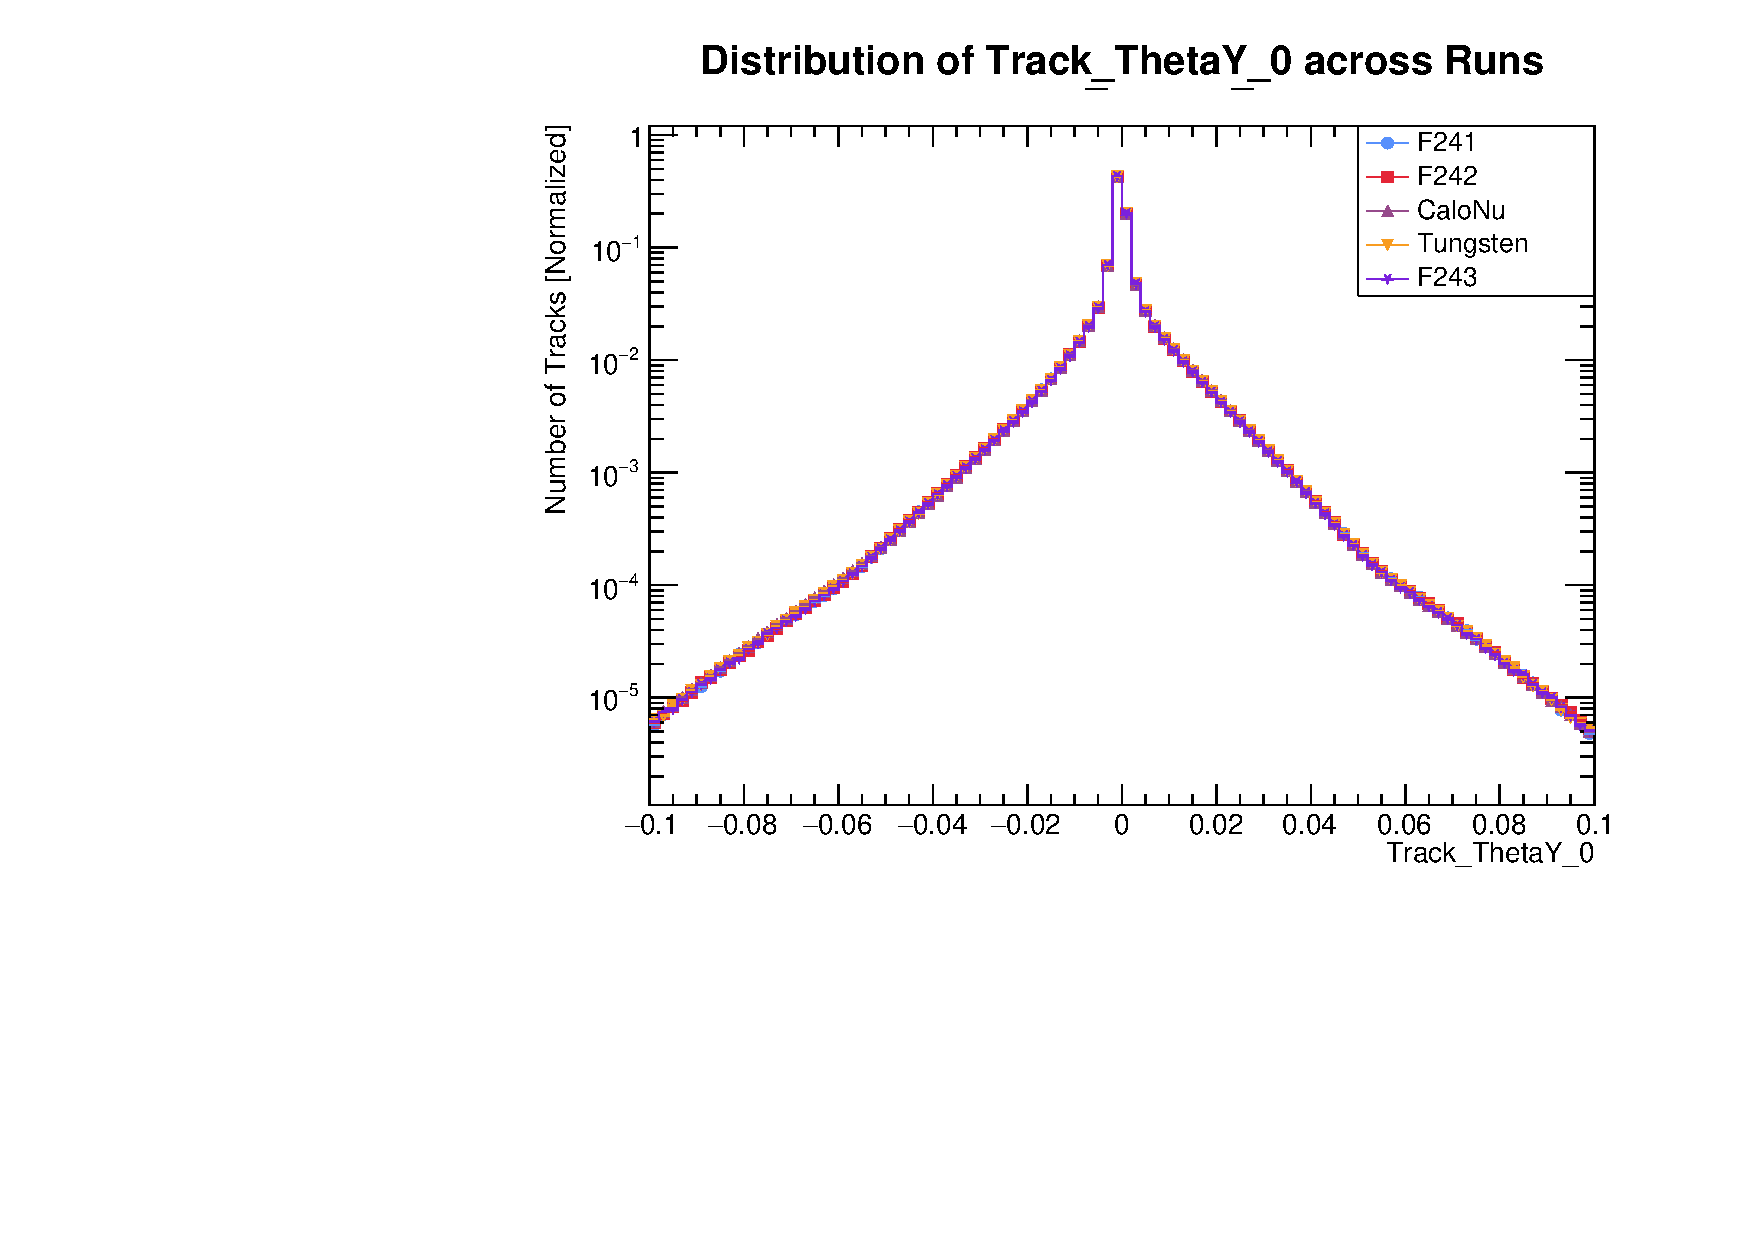
\includegraphics[width=\linewidth]{./RunwisePlots/Track_ThetaY_0_runwise.pdf}
				\caption{Distribution of Track ThetaY0 across 2024 runs}
			\end{figure}
		\end{column}
	\end{columns}
	% \begin{itemize}
	% 	\item General, run-wise agreement is excellent for the Track variables
	% \end{itemize}
\end{frame}


% \begin{frame}{Distribution of Track Angles across 2024 runs}
% 	\begin{columns}
% 		\begin{column}{0.5\linewidth}
% 			\begin{figure}
% 				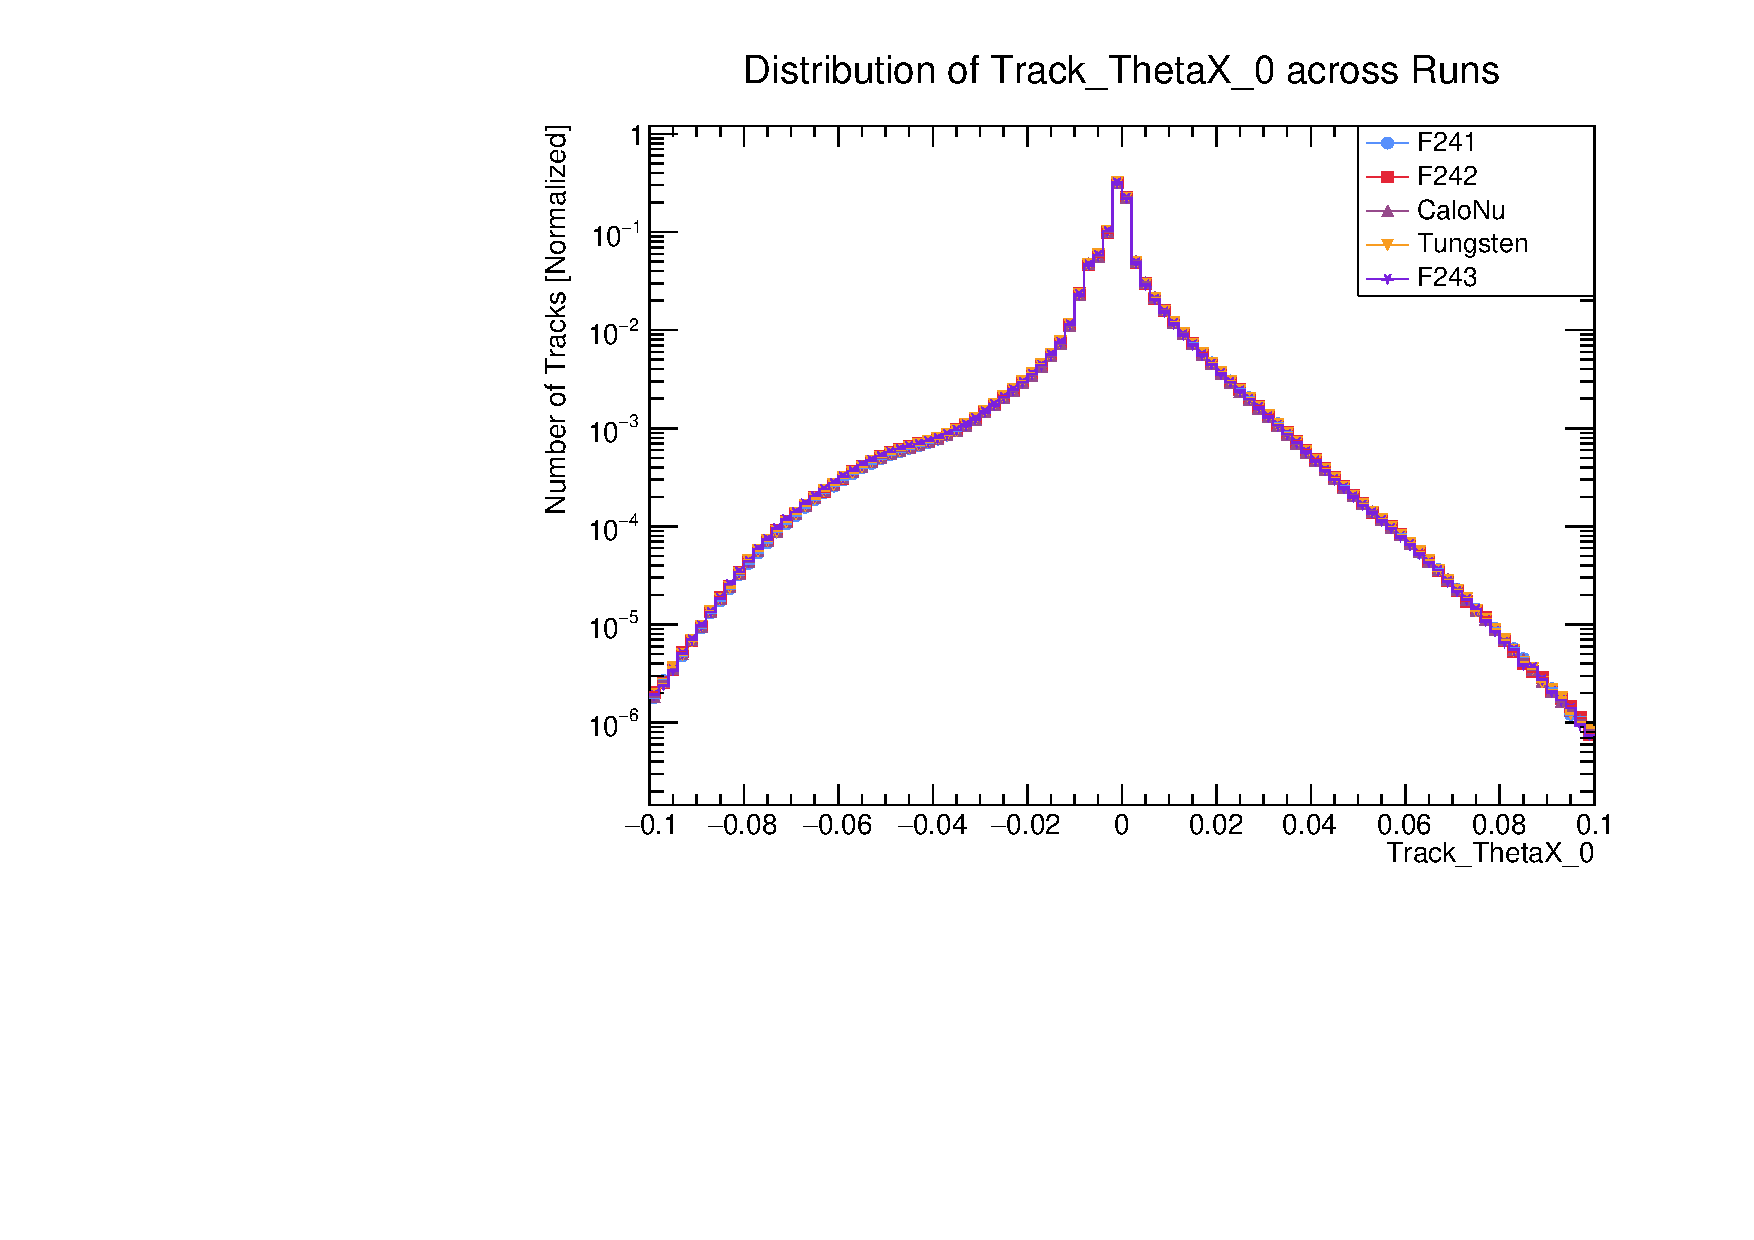
\includegraphics[width=\linewidth]{./RunwisePlots/Track_ThetaX_0_runwise.pdf}
% 				\caption{Distribution of Track ThetaX0 across 2024 runs}
% 			\end{figure}
% 		\end{column}
% 		\begin{column}{0.5 \linewidth}
% 			\begin{figure}
% 				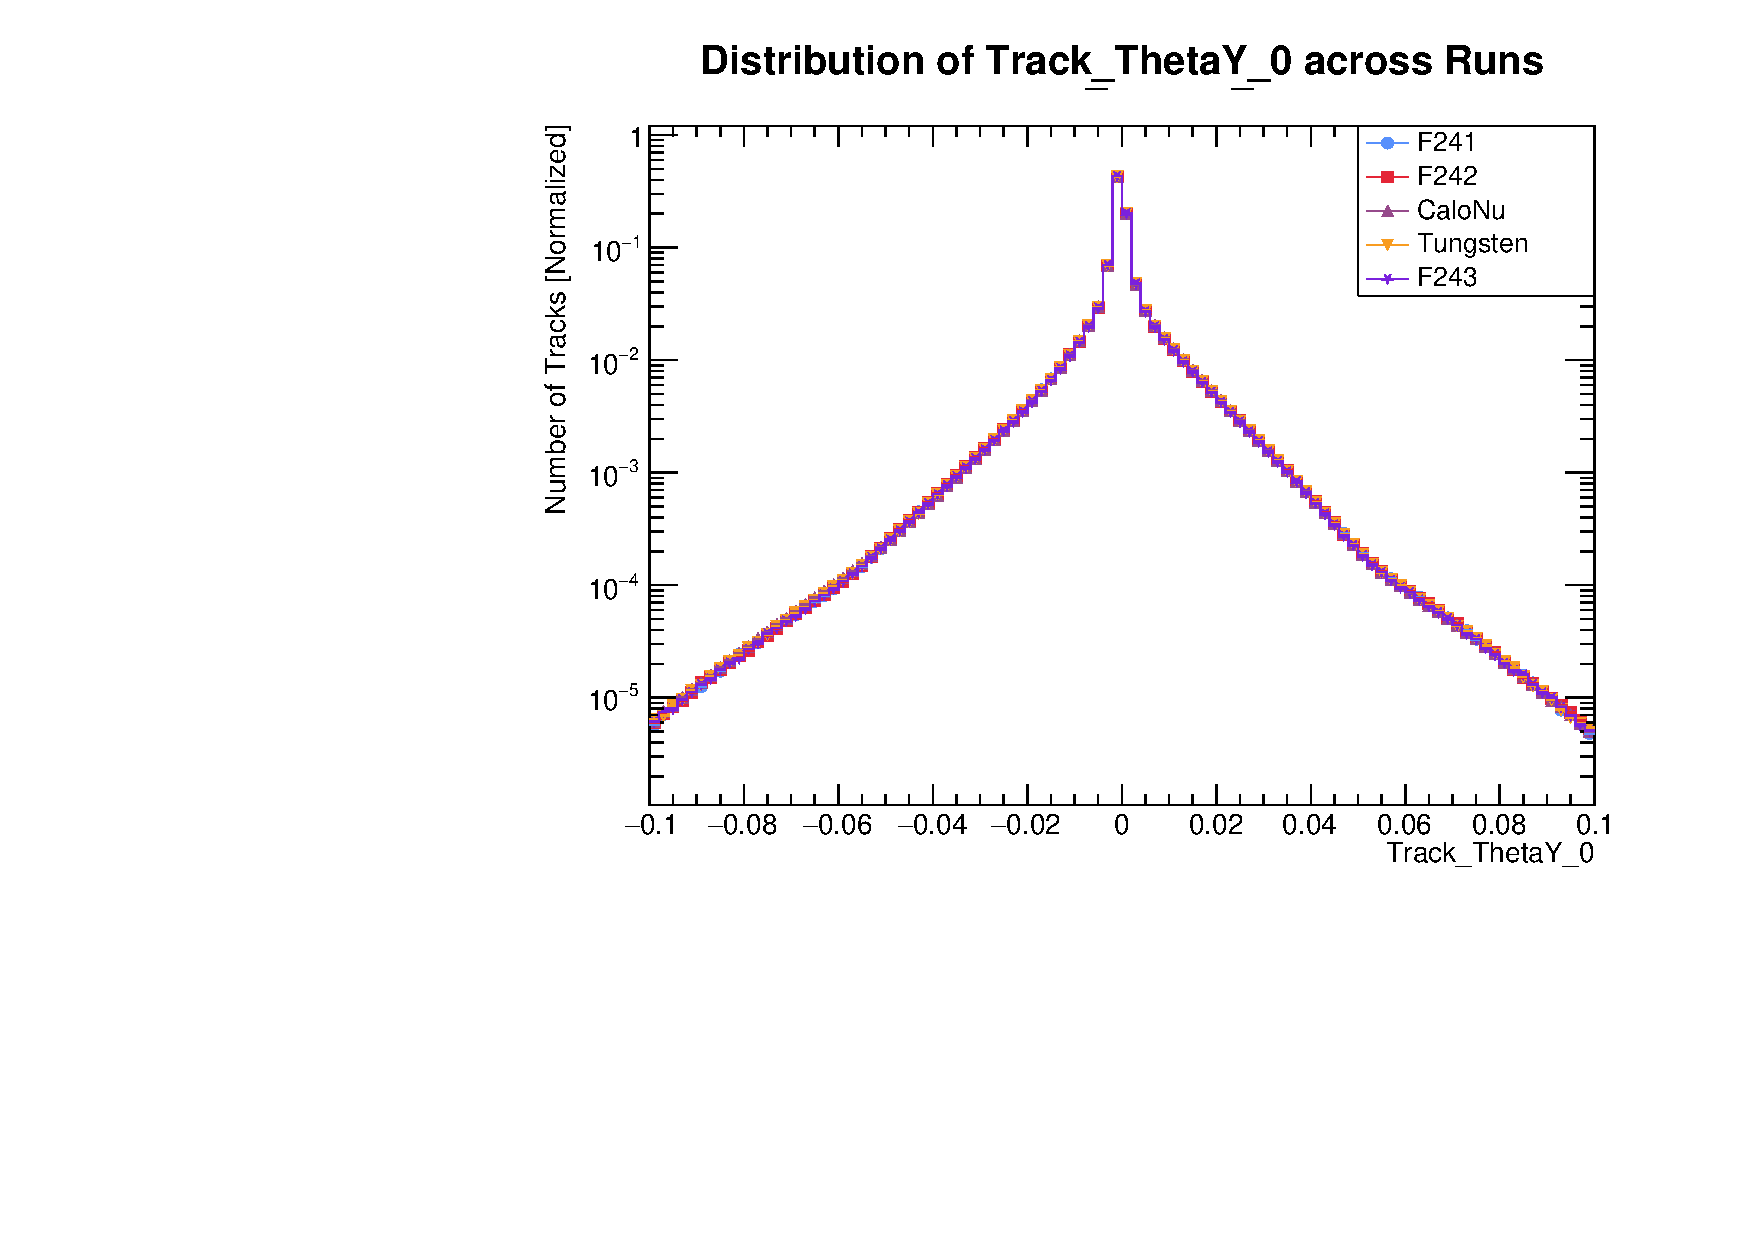
\includegraphics[width=\linewidth]{./RunwisePlots/Track_ThetaY_0_runwise.pdf}
% 				\caption{Distribution of Track ThetaY0 across 2024 runs}
% 			\end{figure}
% 		\end{column}	
% 	\end{columns}
% \end{frame}


\begin{frame}{Distribution of Track Momenta/Charge across runs}
	\begin{columns}
		\begin{column}{0.5\linewidth}
			\begin{figure}
				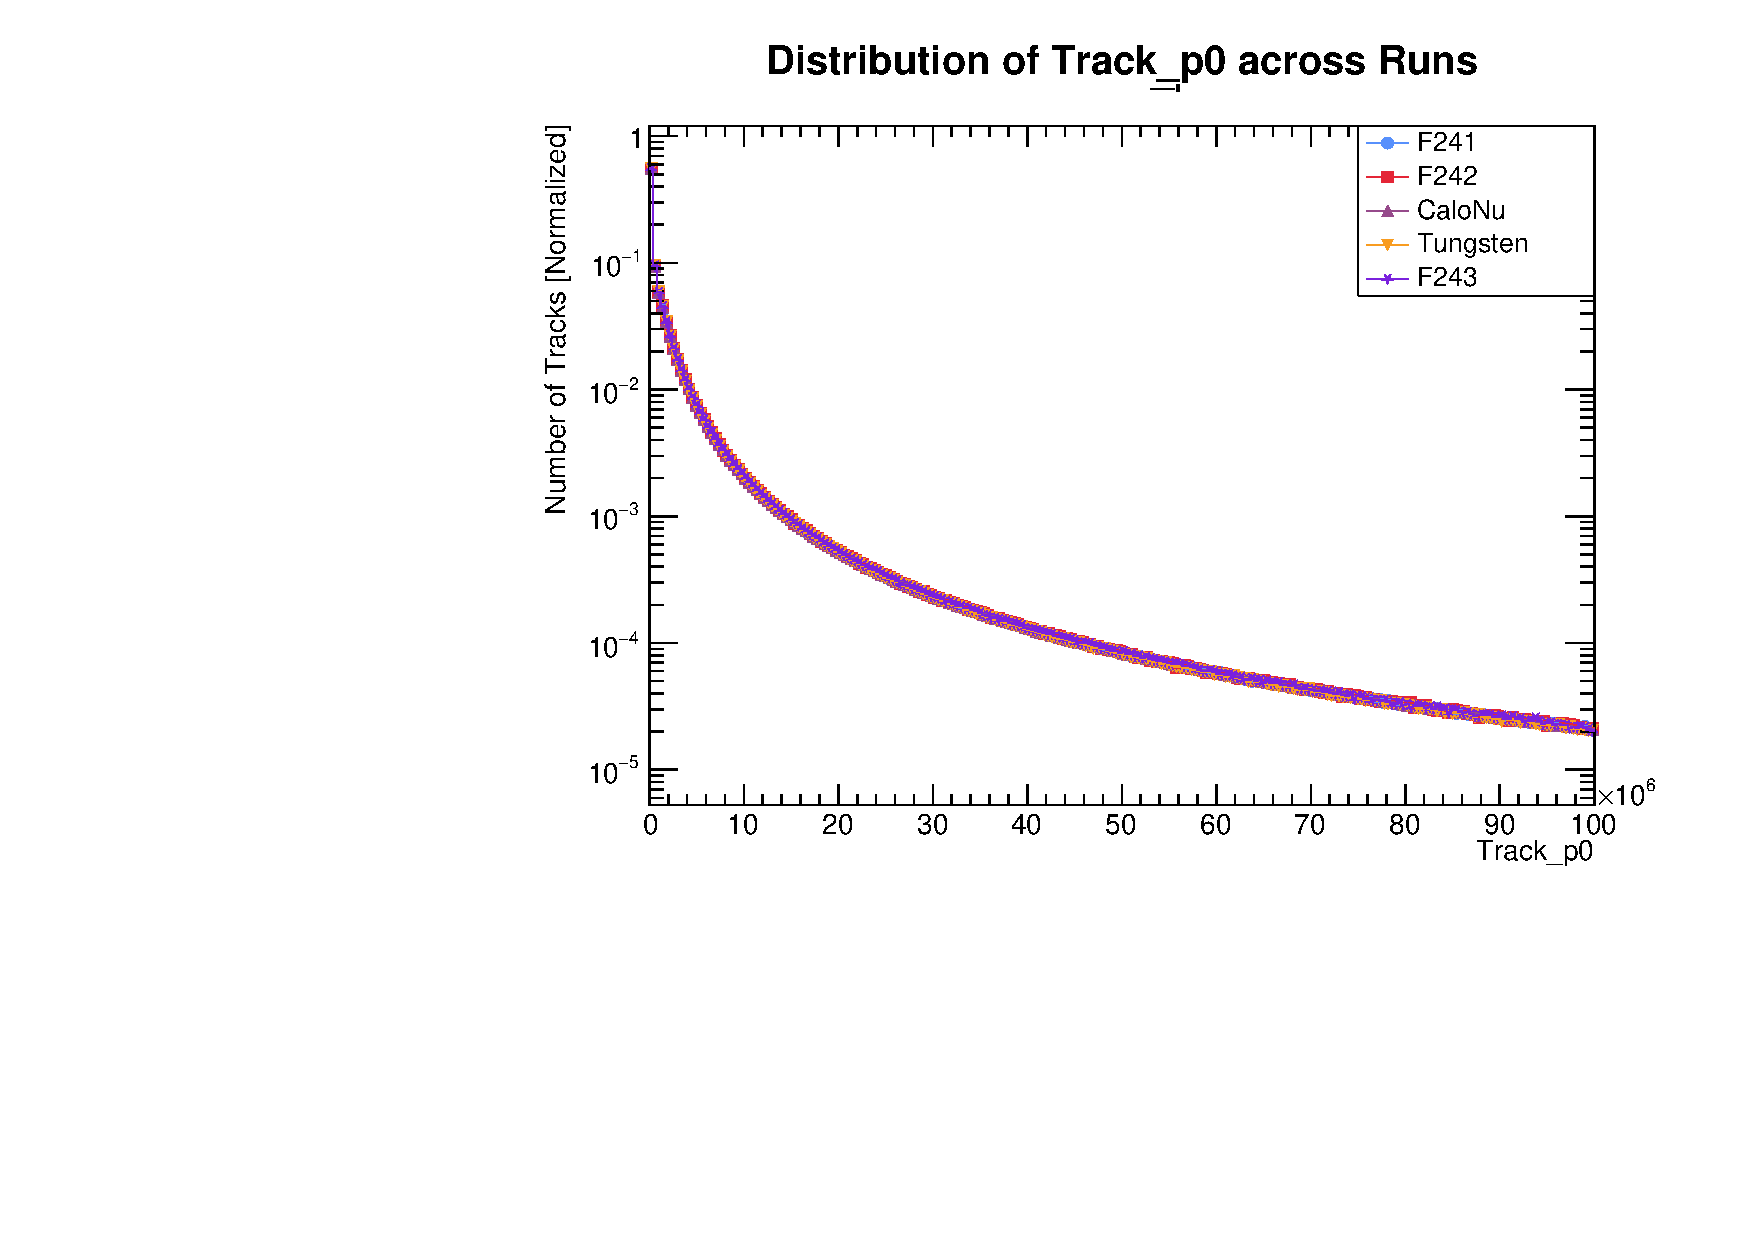
\includegraphics[width=\linewidth]{./RunwisePlots/Track_p0_runwise.pdf}
				\caption{Distribution of Track Momenta in MeV across 2024 runs, as measured by the first tracking station}
			\end{figure}
		\end{column}
		\begin{column}{0.5\linewidth}
			\begin{figure}
				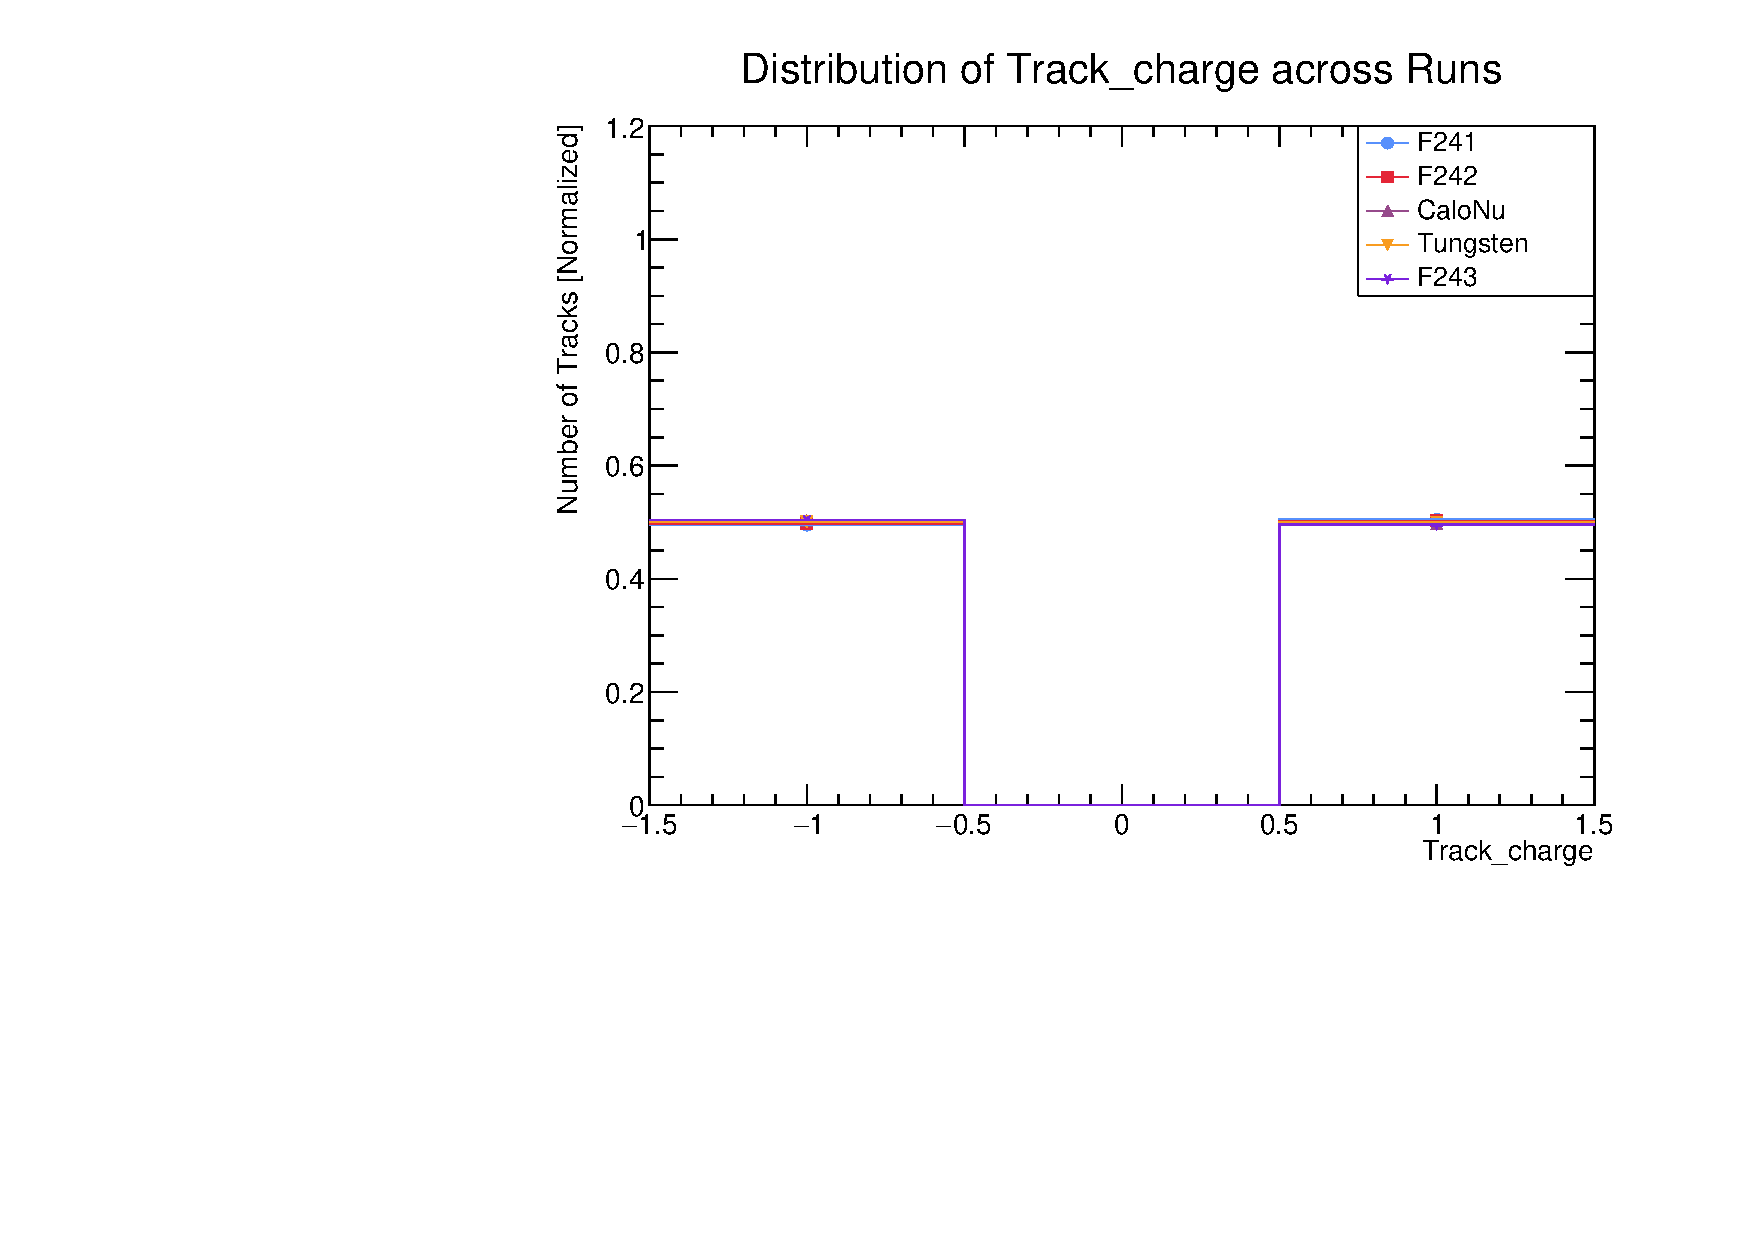
\includegraphics[width=\linewidth]{./RunwisePlots/Track_charge_runwise.pdf}
				\caption{Distribution of Track Charge across 2024 runs}
			\end{figure}
		\end{column}
	\end{columns}
	\begin{itemize}
		\item The background seems consistent across the runs as well.
		\item Really good agreement across runs for all tracking parameters (Track $\chi^{2}$ etc) across the five 2024 run periods.
	\end{itemize}
\end{frame}

\begin{frame}{Distribution of longTracks across 2024 runs}
	\begin{columns}
		\begin{column}{0.55 \linewidth}
			\begin{figure}
				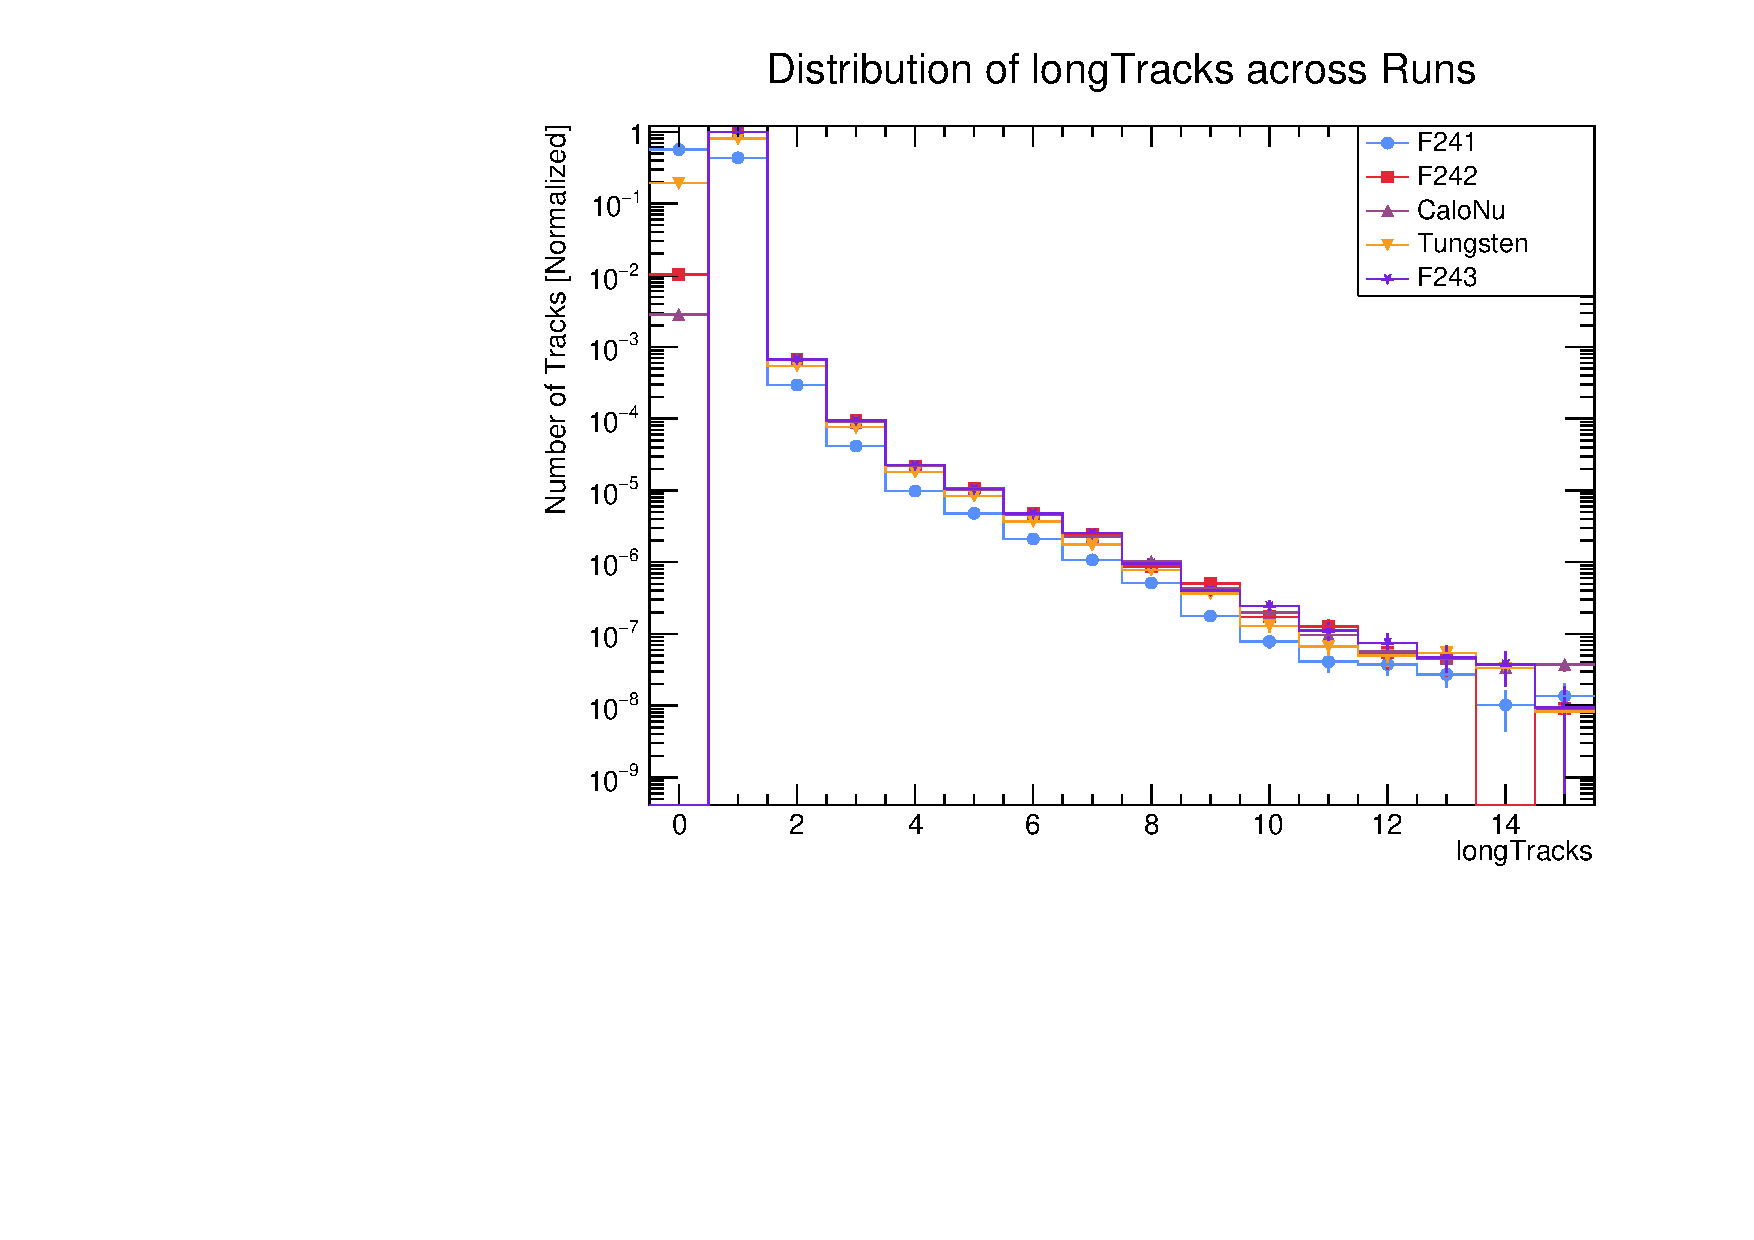
\includegraphics[width=\linewidth]{./RunwisePlots/longTracks_runwise.pdf}
				\caption{LongTracks across 2024 runs [Normalized to Sum of Entries across all bins]}
			\end{figure}
		\end{column}
		\begin{column}{0.55 \linewidth}
			\begin{figure}
				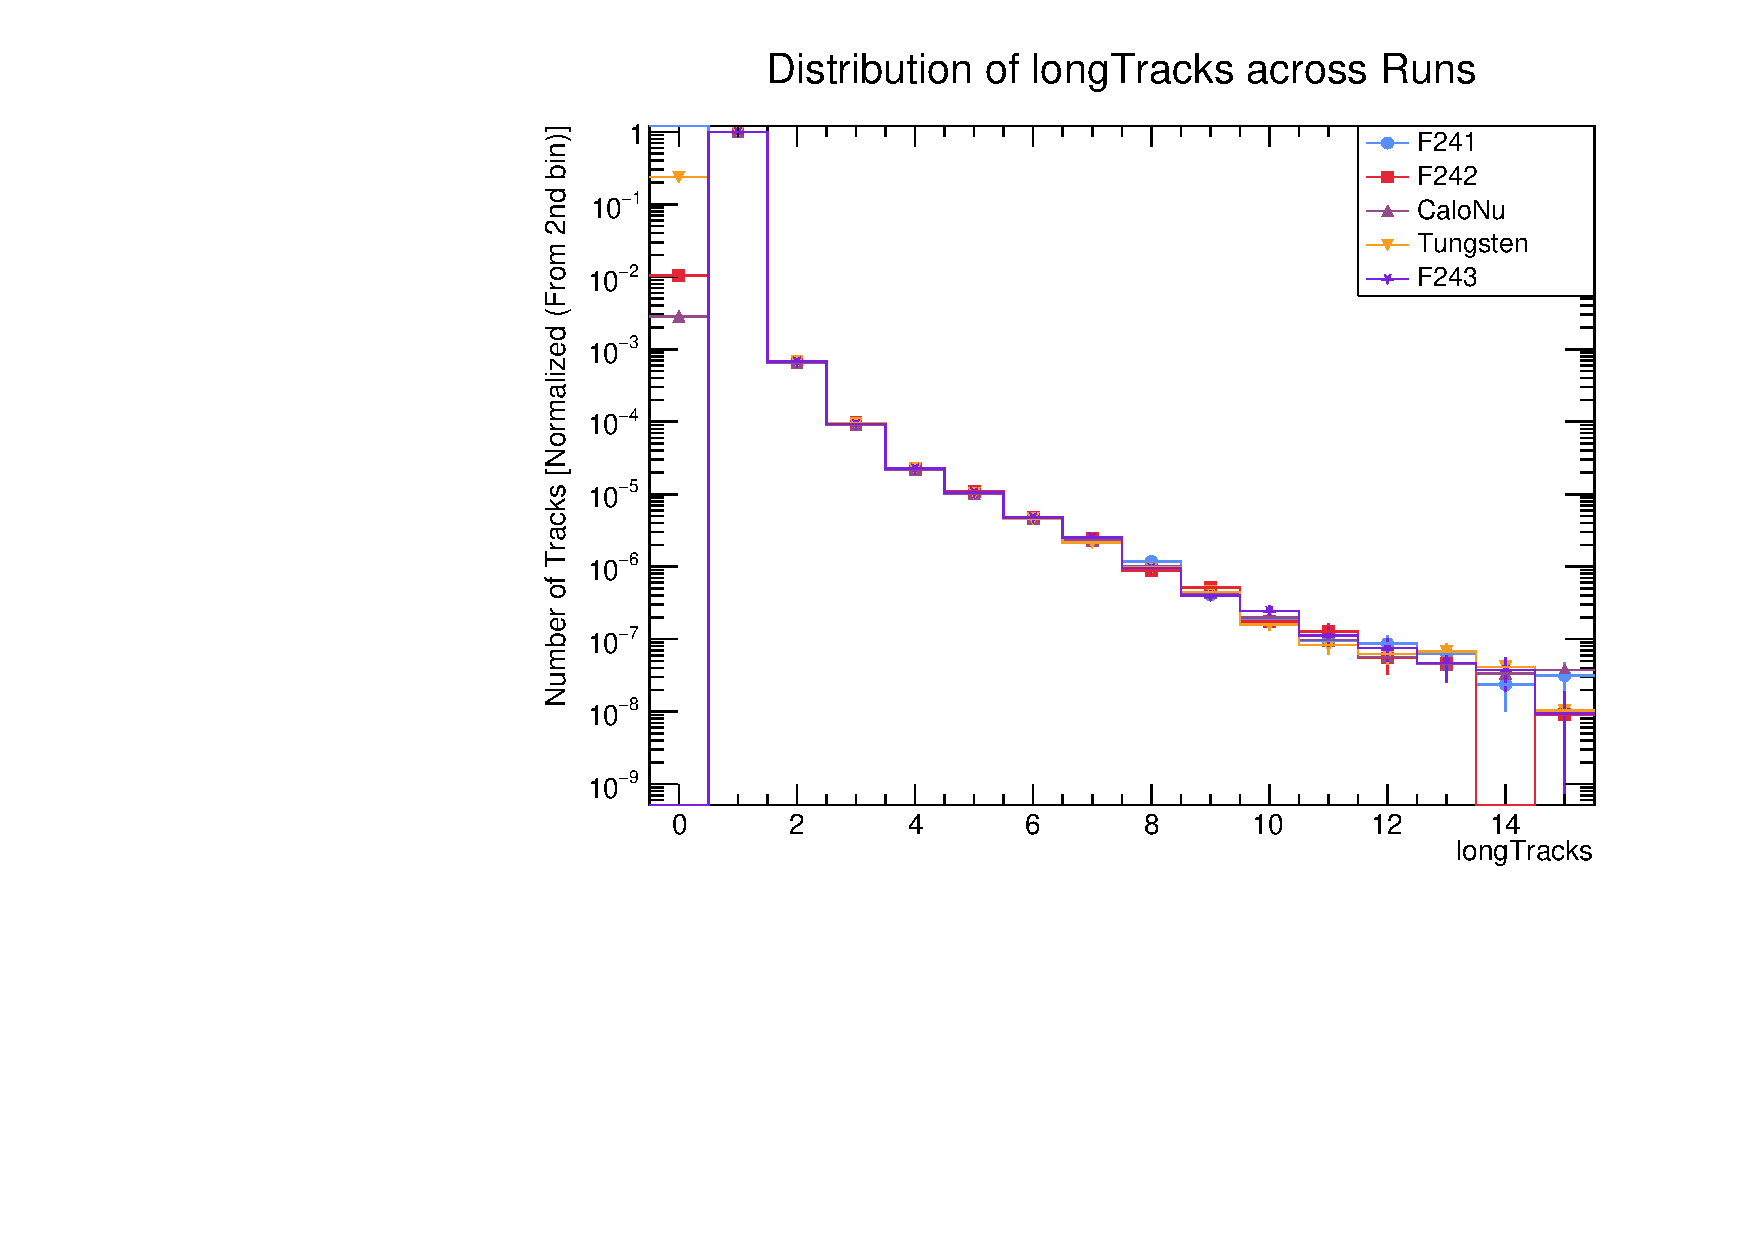
\includegraphics[width=\linewidth]{RunwisePlots/longTracks_normalisedfrom2_runwise.pdf}
				\caption{LongTracks across 2024 runs [Normalized to Sum of Entries starting from 2nd bin]}
			\end{figure}
		\end{column}
	\end{columns}
	\begin{itemize}
		\item F241 seems to show a higher number of 0-longTrack events.
		\item Most likely from the lack of BCID cut for the early runs (less bunches) in F241.
	\end{itemize}
	% \begin{figure}
	% 	\begin{subfigure}{0.45\linewidth}
	% 		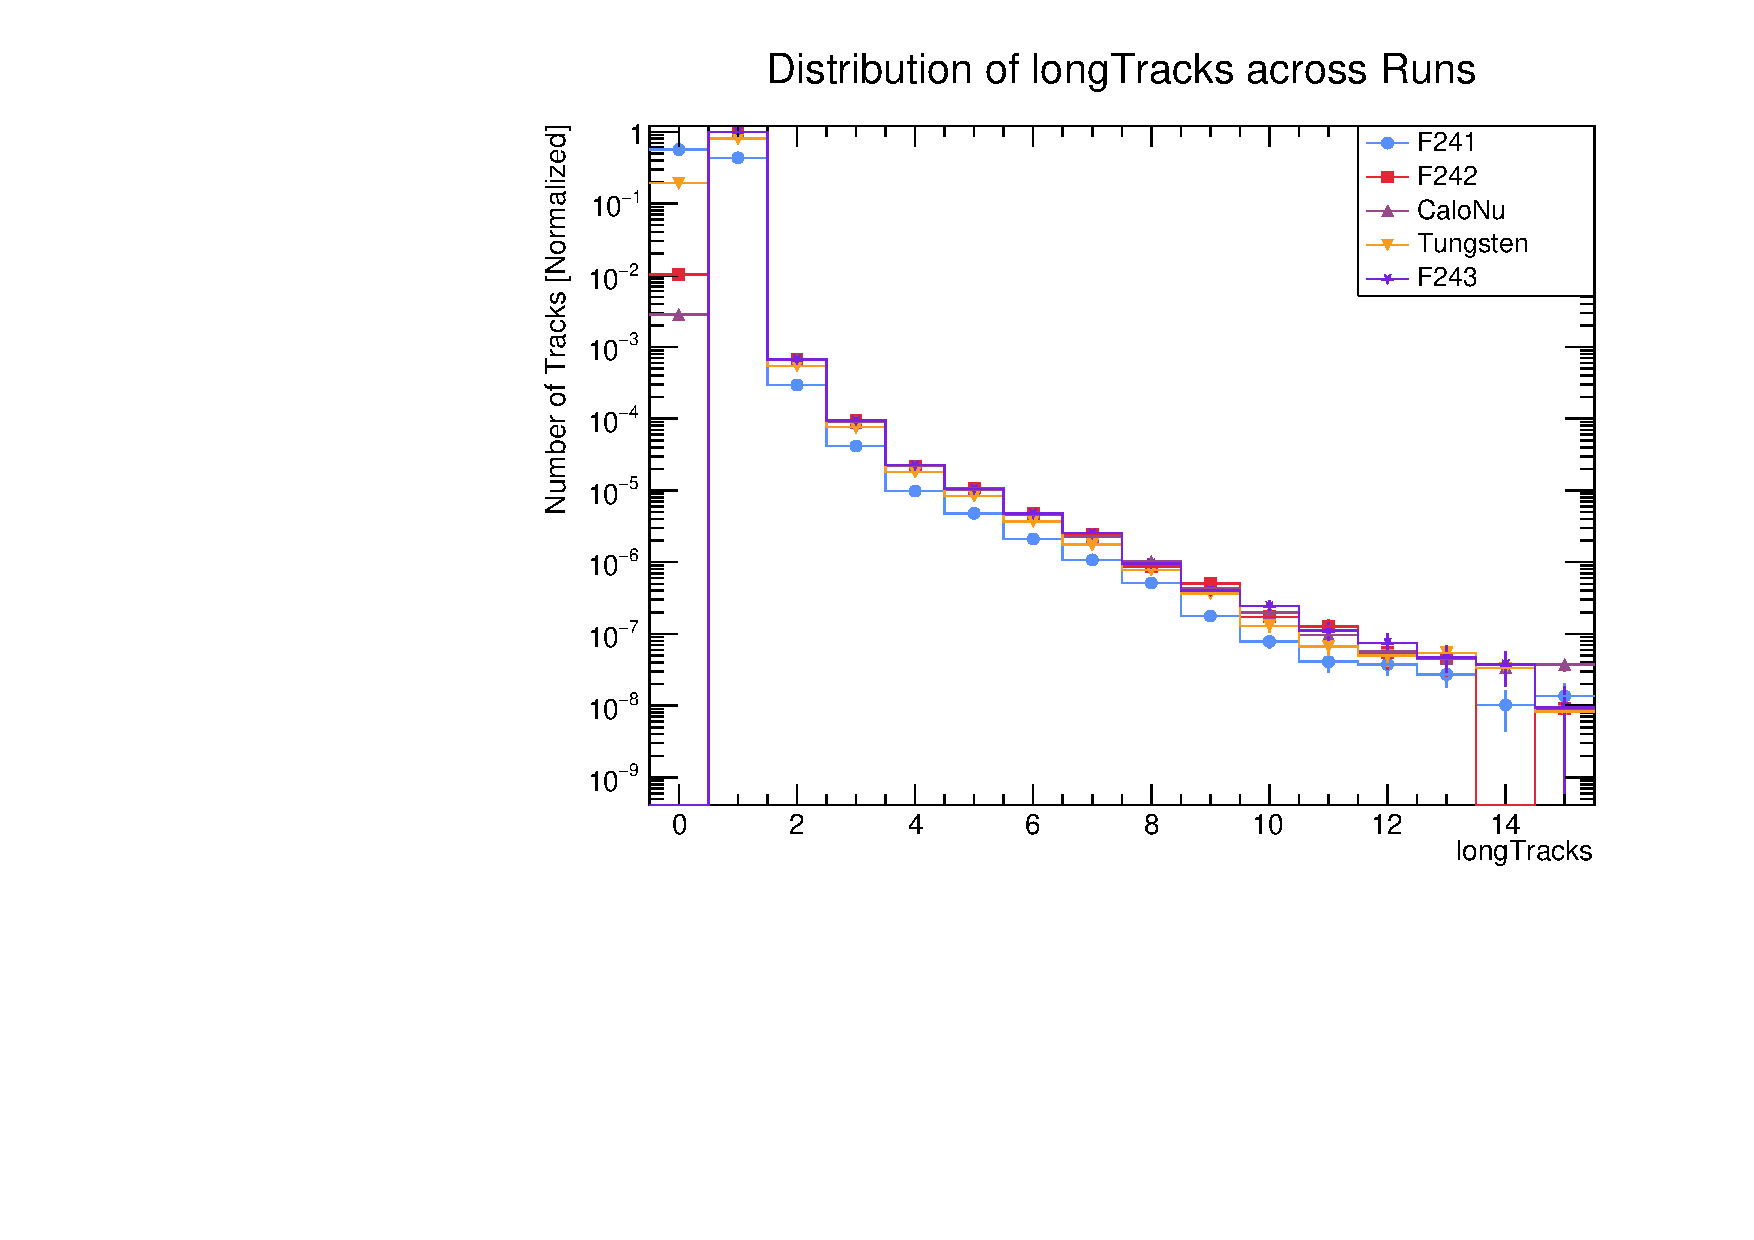
\includegraphics[width=1.2\linewidth]{./RunwisePlots/longTracks_runwise.pdf}
	% 	\end{subfigure}
	% 	\begin{subfigure}{0.45\linewidth}
	% 		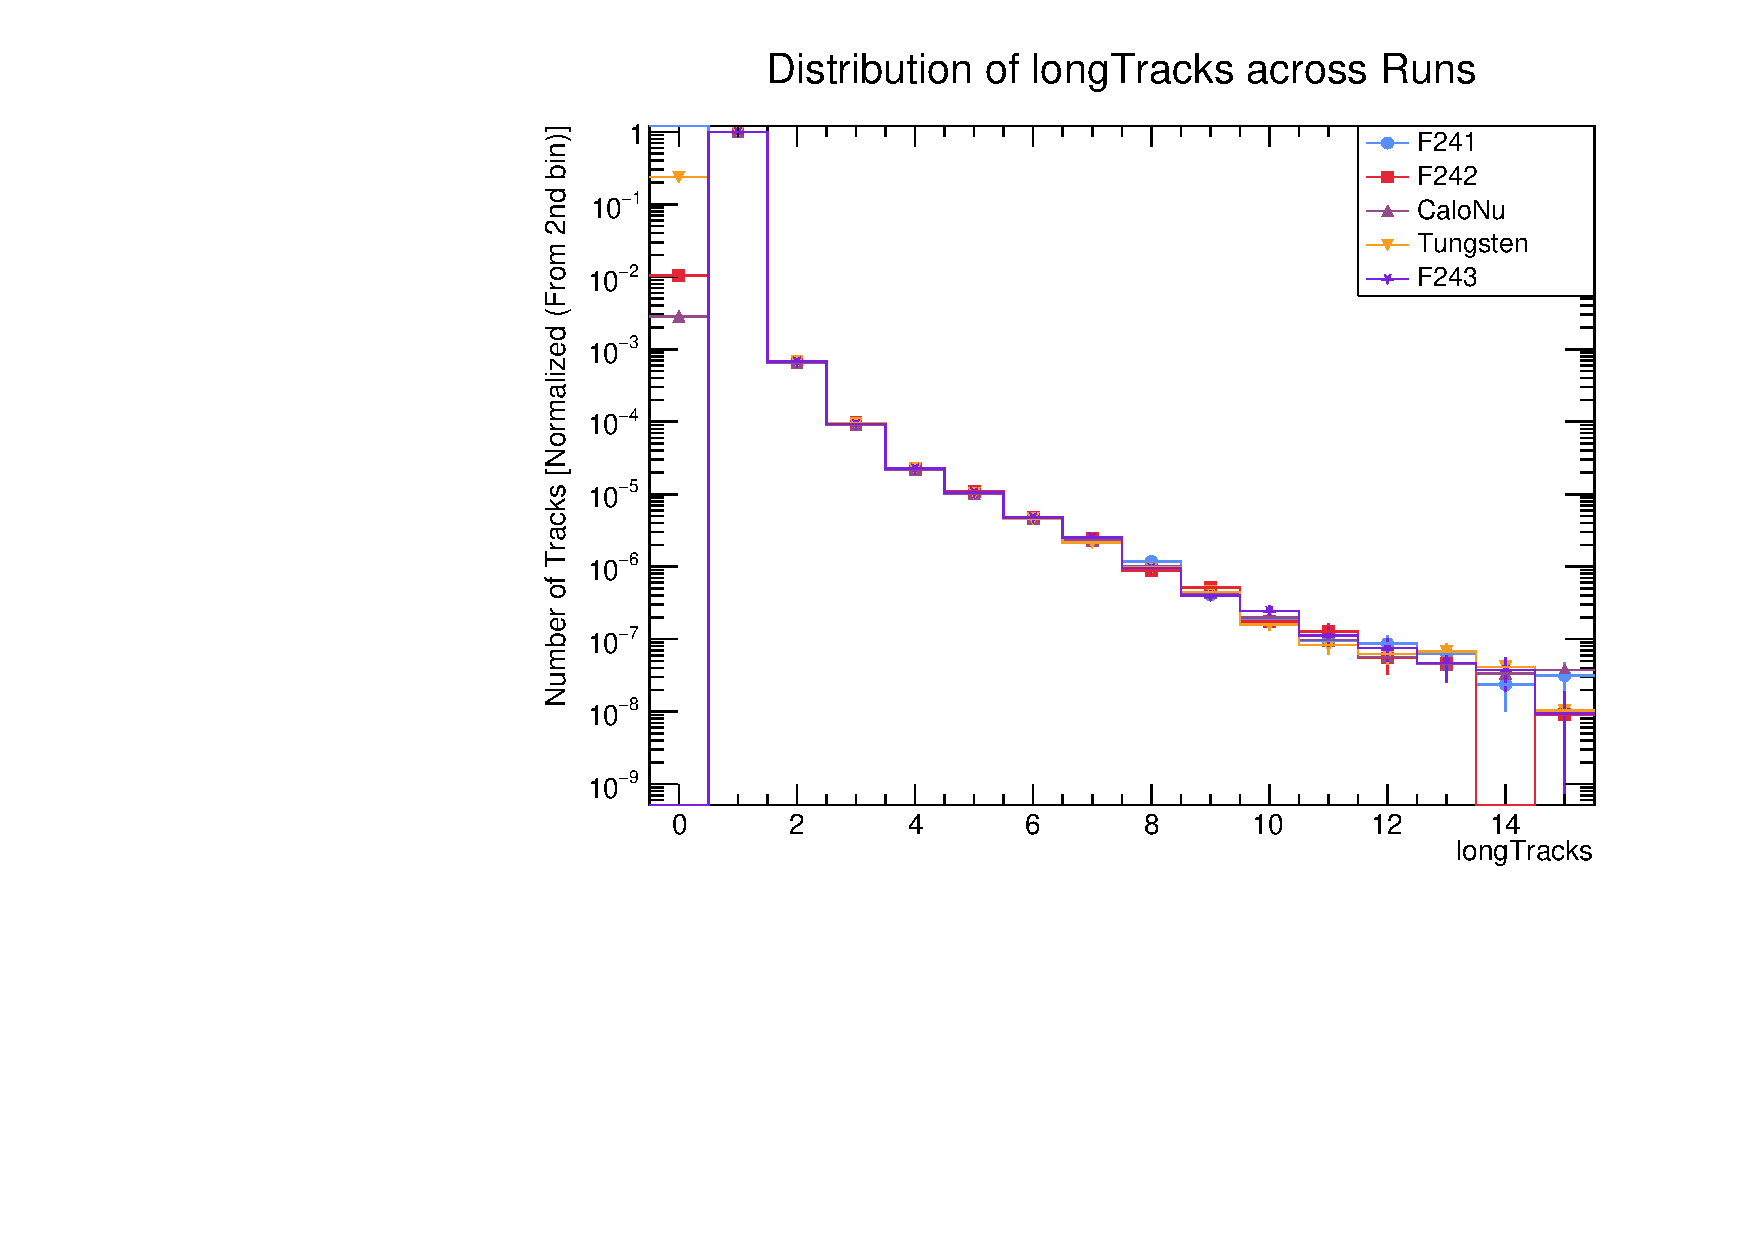
\includegraphics[width=1.2\linewidth]{RunwisePlots/longTracks_normalisedfrom2_runwise.pdf}
	% 	\end{subfigure}
	% \end{figure}
\end{frame}

% \begin{frame}{Track Charge across 2024 runs}
% 	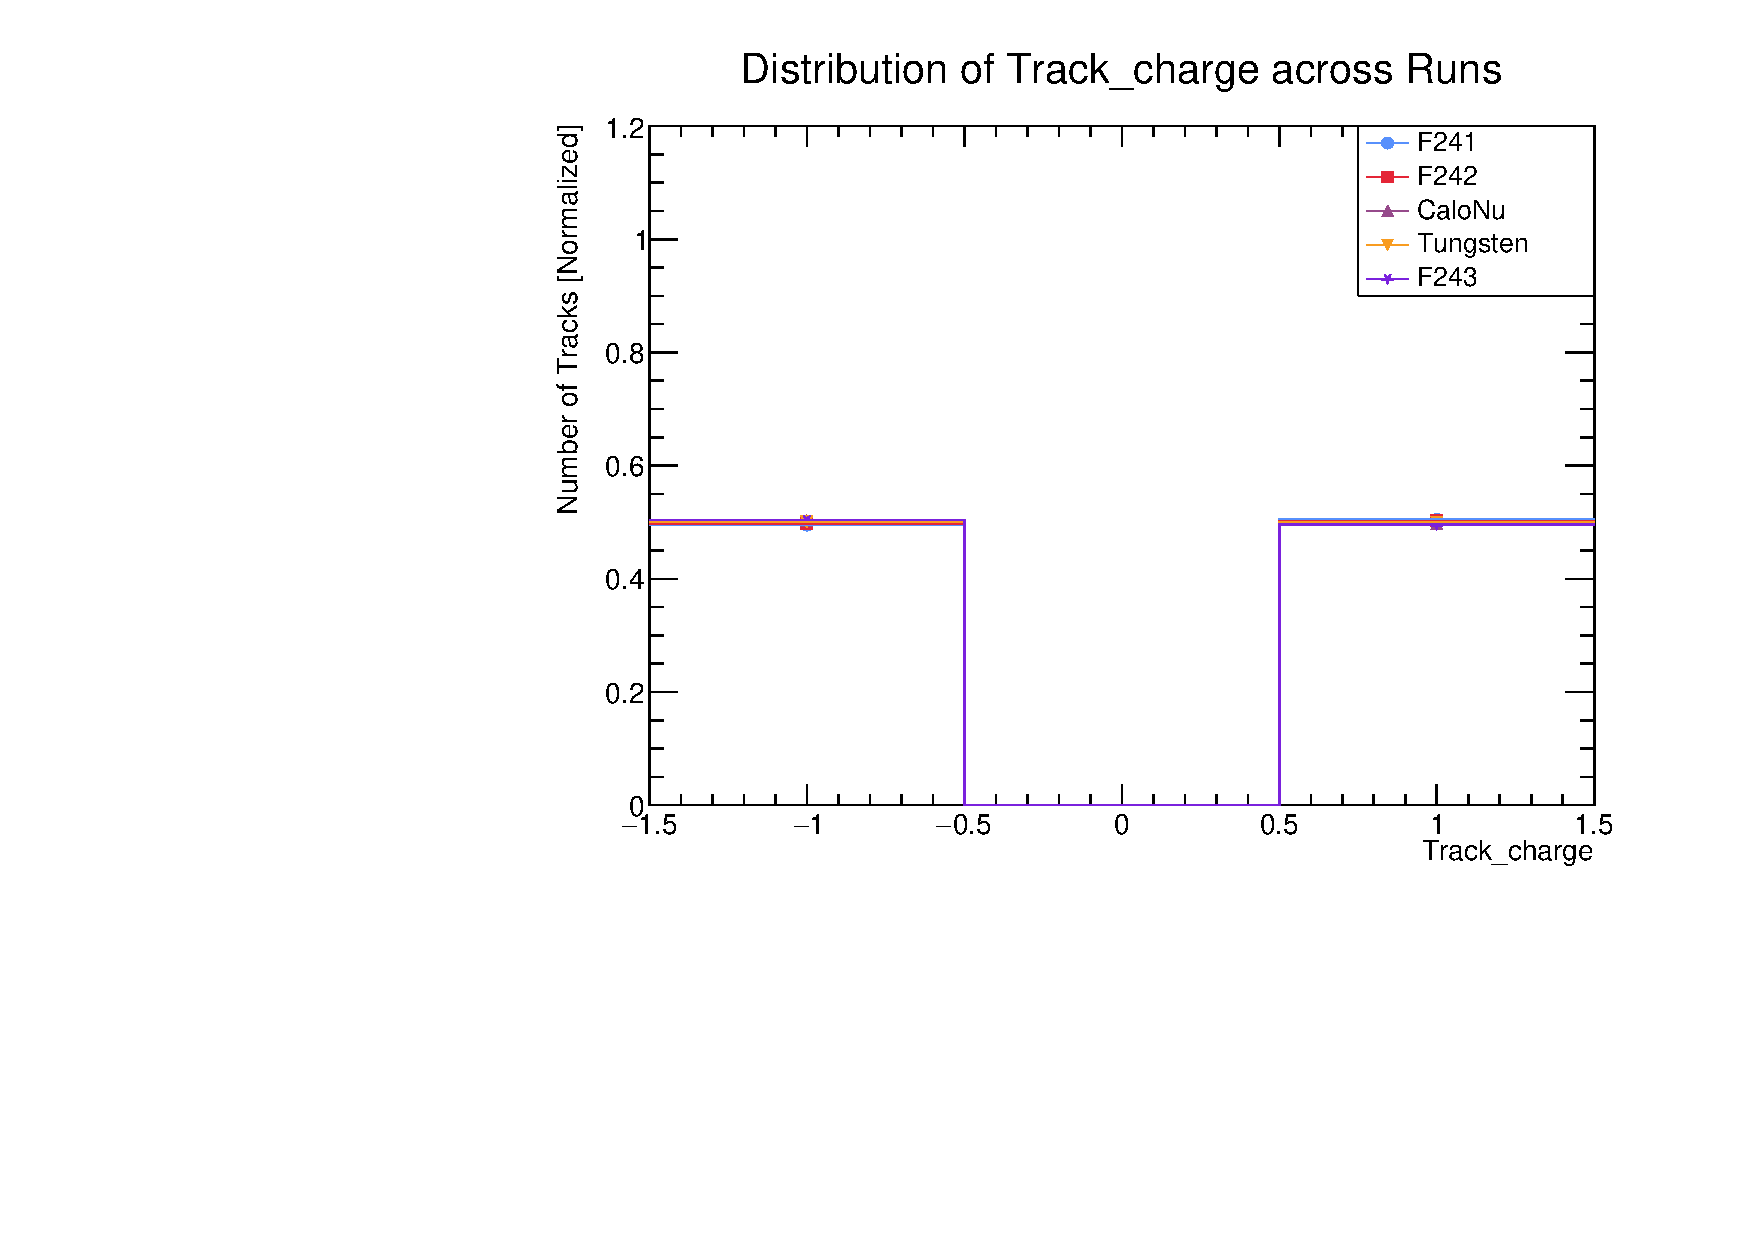
\includegraphics[width=\linewidth]{./RunwisePlots/Track_charge_runwise.pdf}
% \end{frame}

% \begin{frame}{Track Chi2/nDoF across 2024 runs}
% 	\begin{columns}
% 		\begin{column}{0.5 \linewidth}
% 			\vspace{-0.4cm}
% 			\begin{figure}
% 				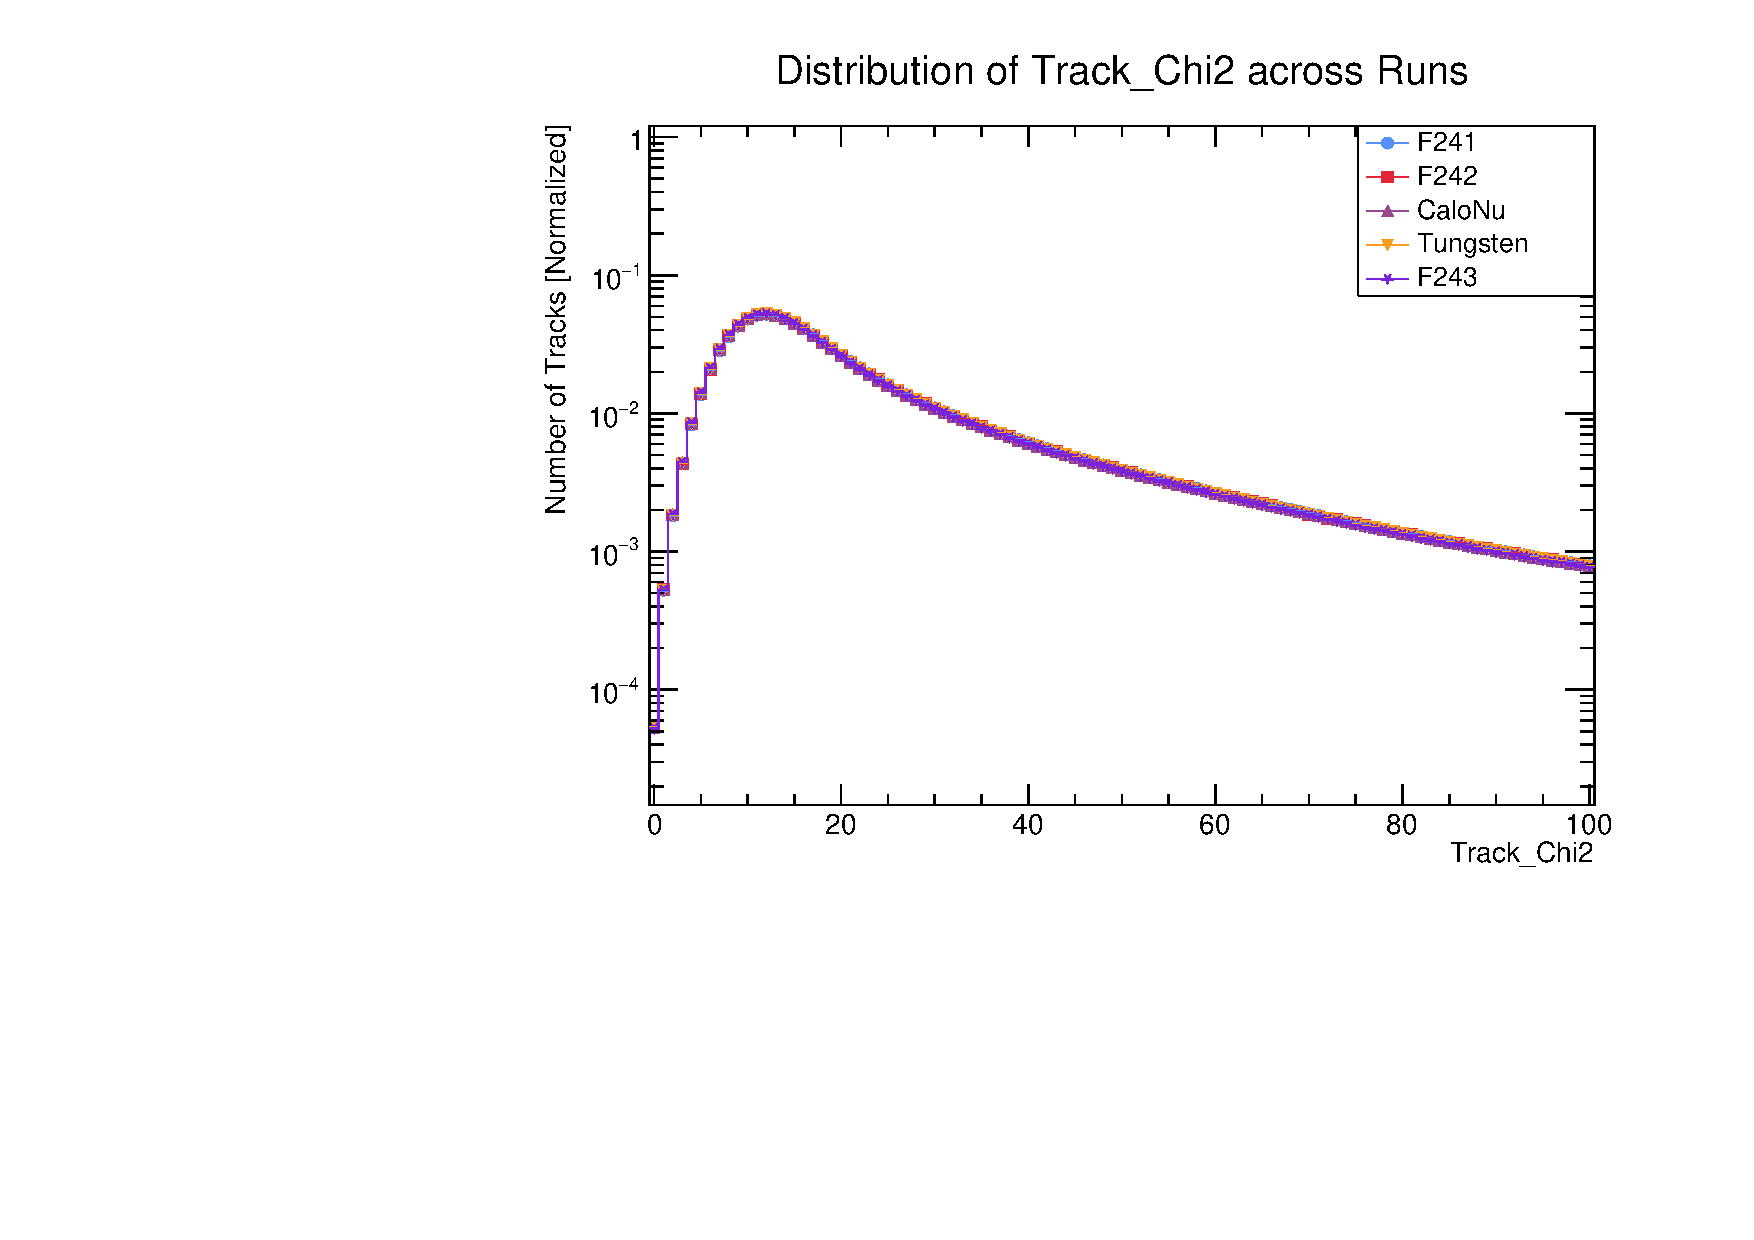
\includegraphics[width=\linewidth]{./RunwisePlots/Track_Chi2_runwise.pdf}
% 				% \caption{Distribution of Track Chi2 across 2024 runs}
% 			\end{figure}
% 			\vspace{-0.6cm}
% 			\begin{figure}
% 				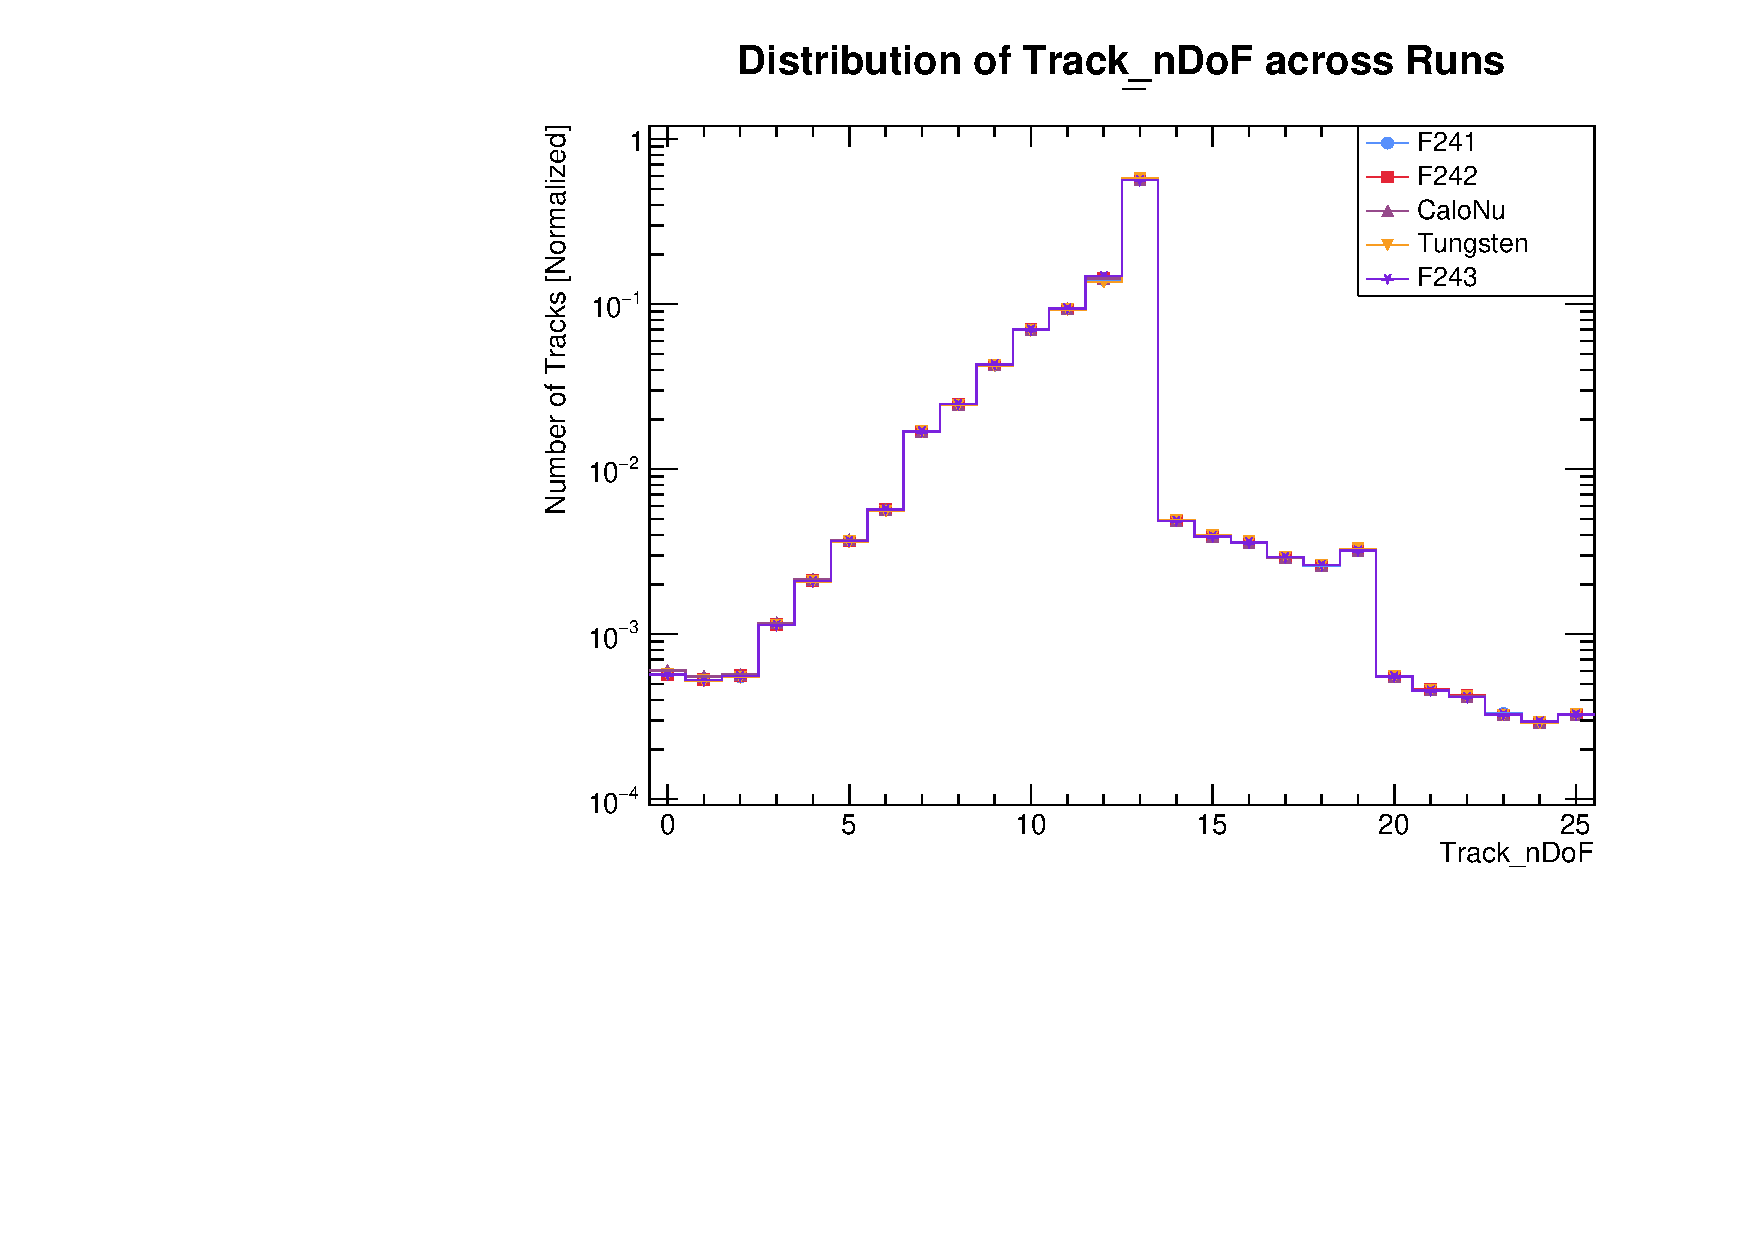
\includegraphics[width=\linewidth]{./RunwisePlots/Track_nDoF_runwise.pdf}
% 			\end{figure}
% 		\end{column}
% 		\begin{column}{0.5 \linewidth}
% 			\begin{figure}
% 				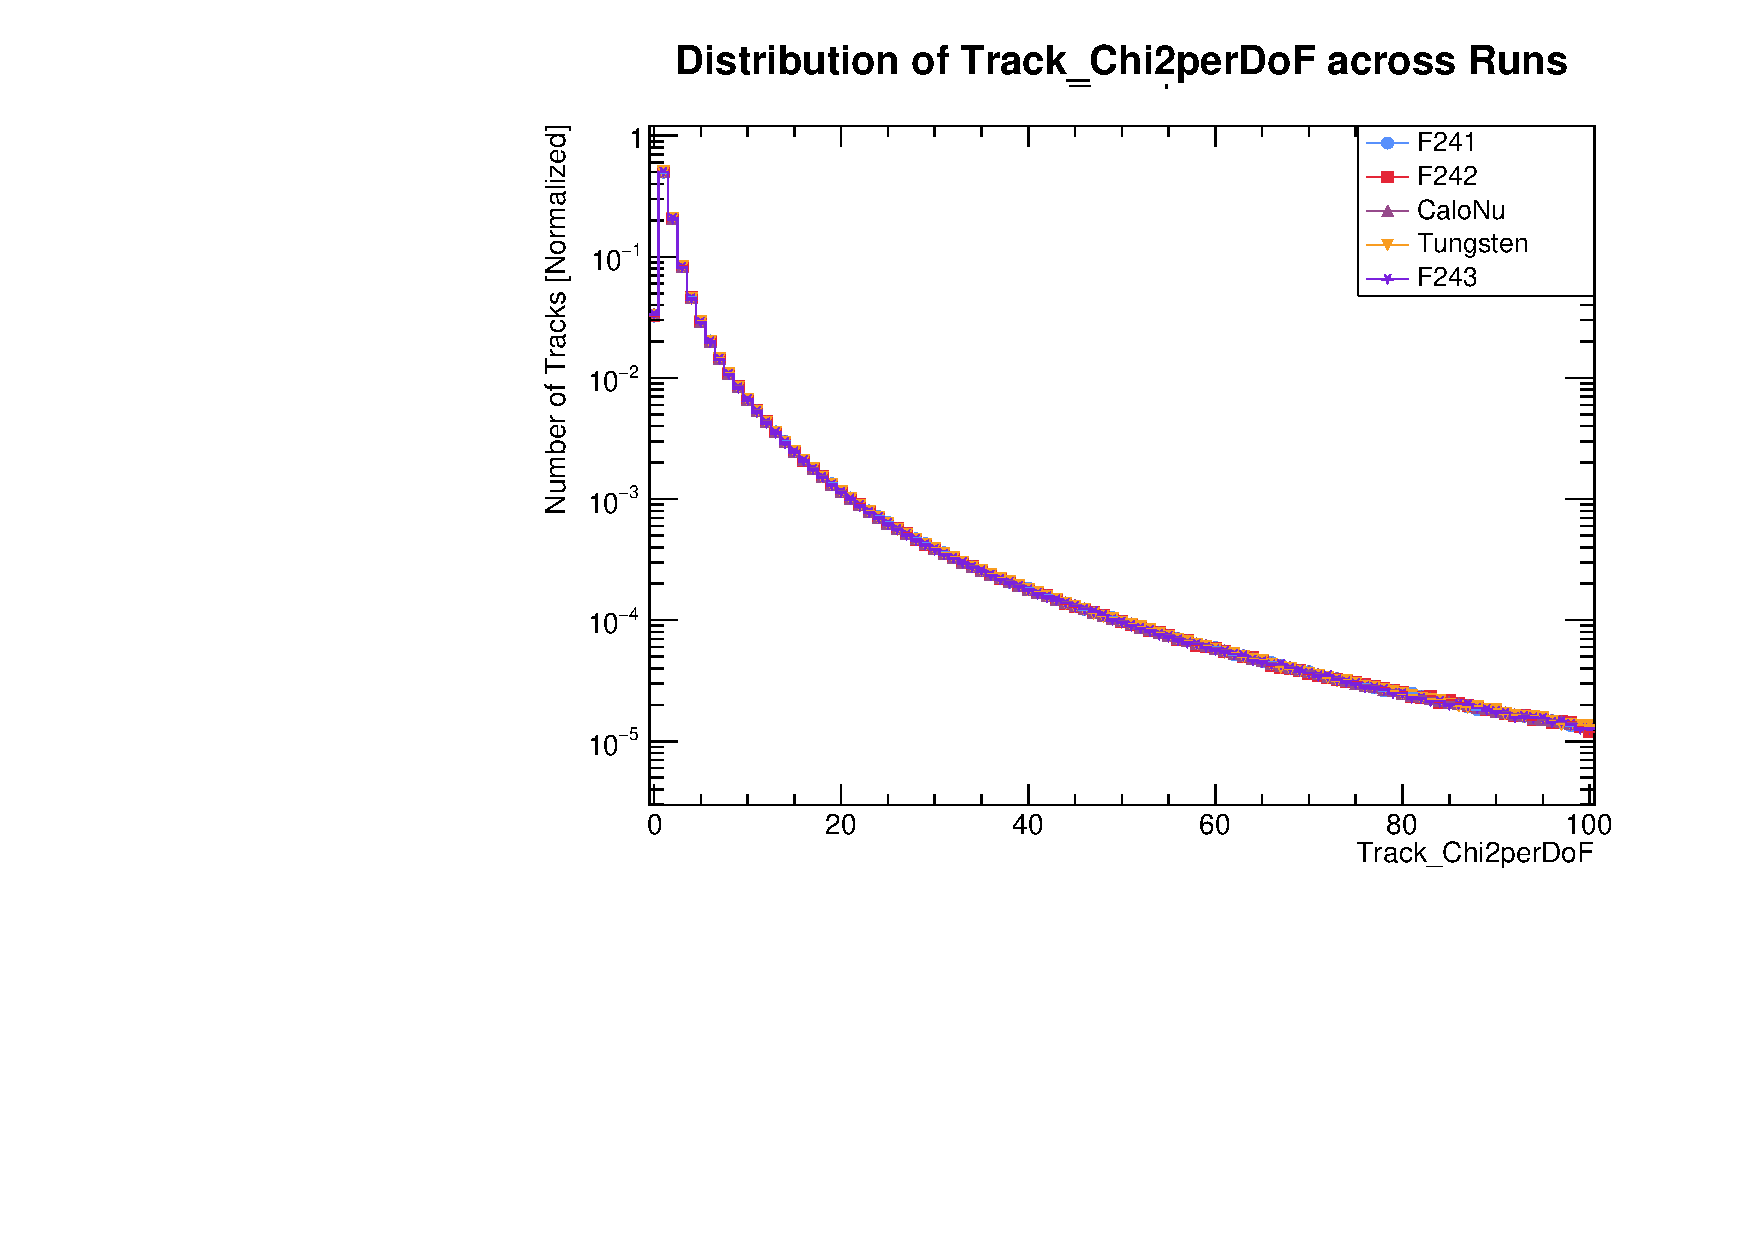
\includegraphics[width=\linewidth]{./RunwisePlots/Track_Chi2perDoF_runwise.pdf}
% 				\caption{Distribution of Track Chi2/DoF across 2024 runs}
% 			\end{figure}
% 		\end{column}
% 	\end{columns}
% \end{frame}

% \begin{frame}{Track nDoF and nLayers across 2024 runs}
% 	\begin{columns}
% 		\begin{column}{0.5\linewidth}
% 			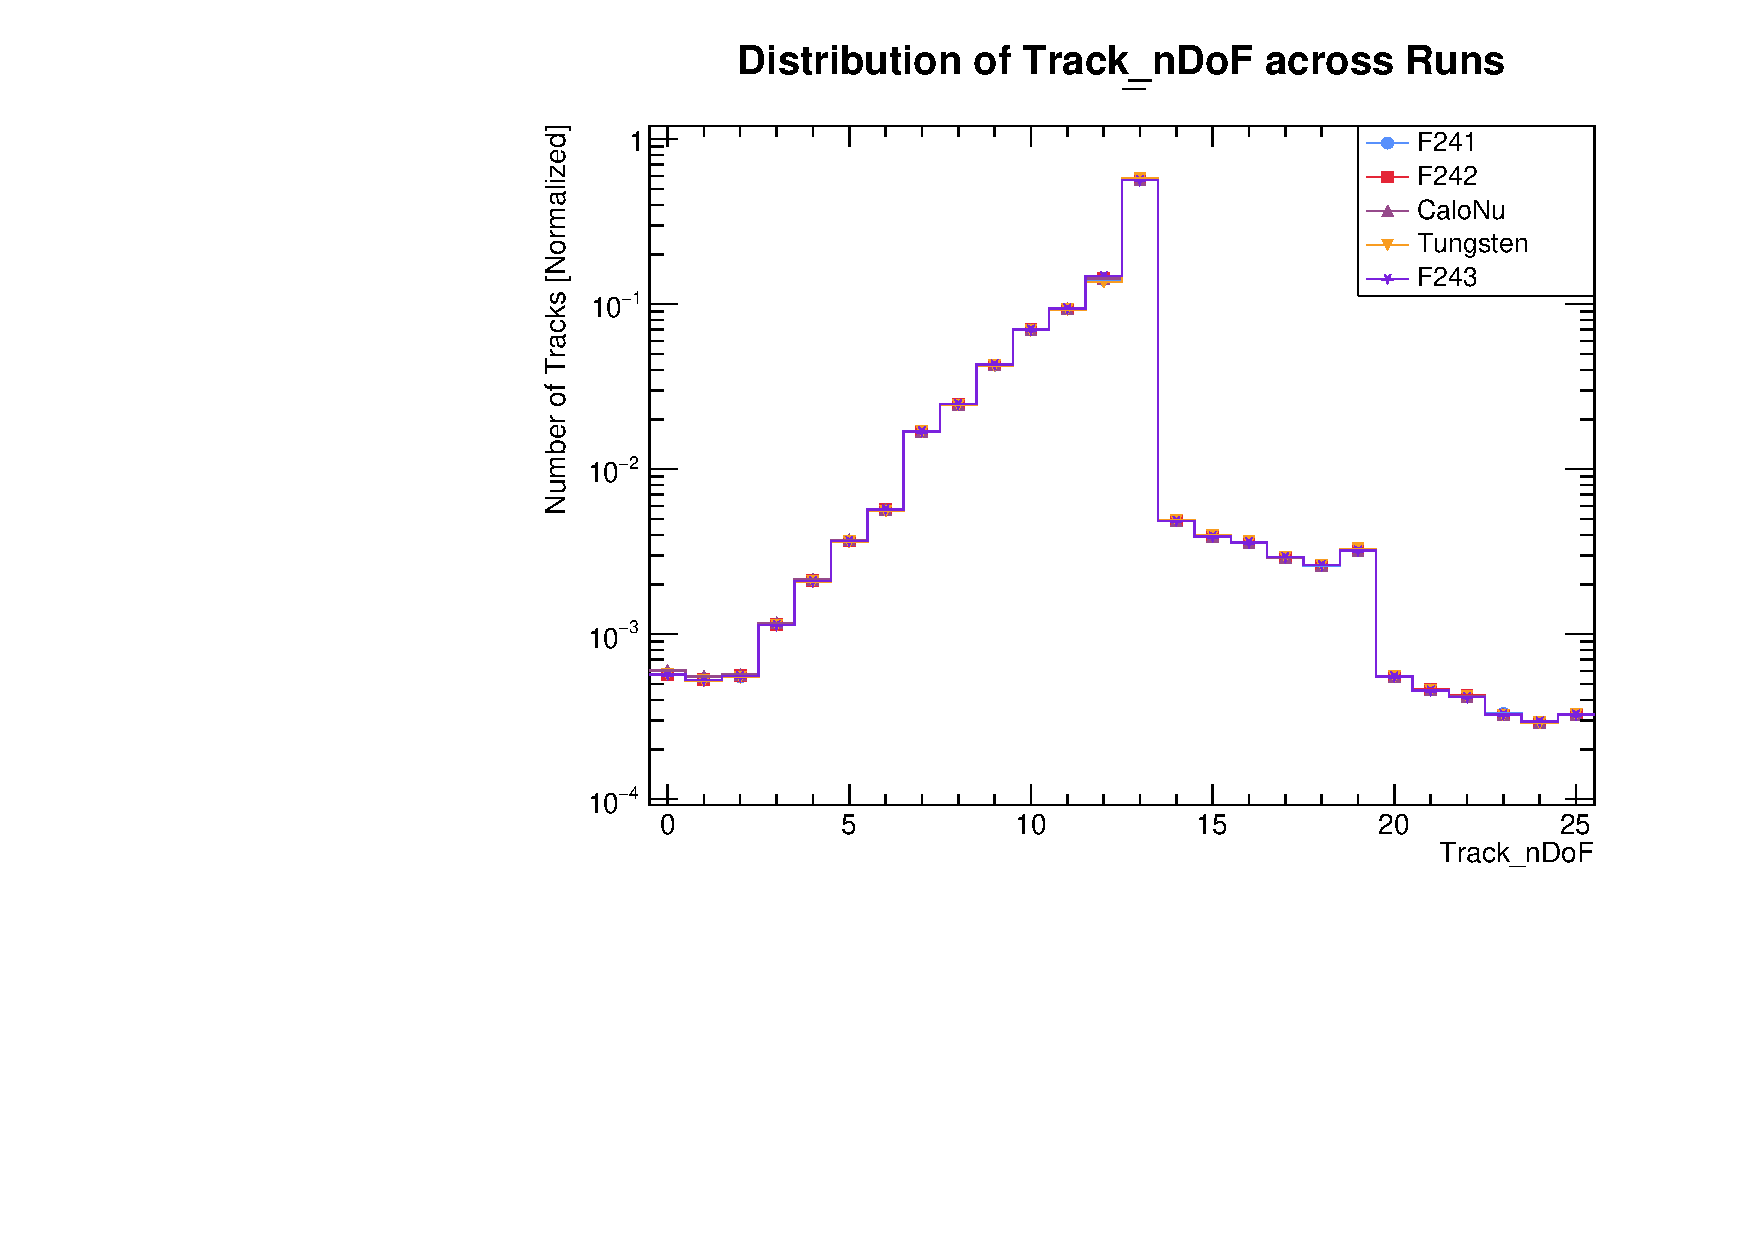
\includegraphics[width=\linewidth]{./RunwisePlots/Track_nDoF_runwise.pdf}
% 		\end{column}
% 		\begin{column}{0.5\linewidth}
% 			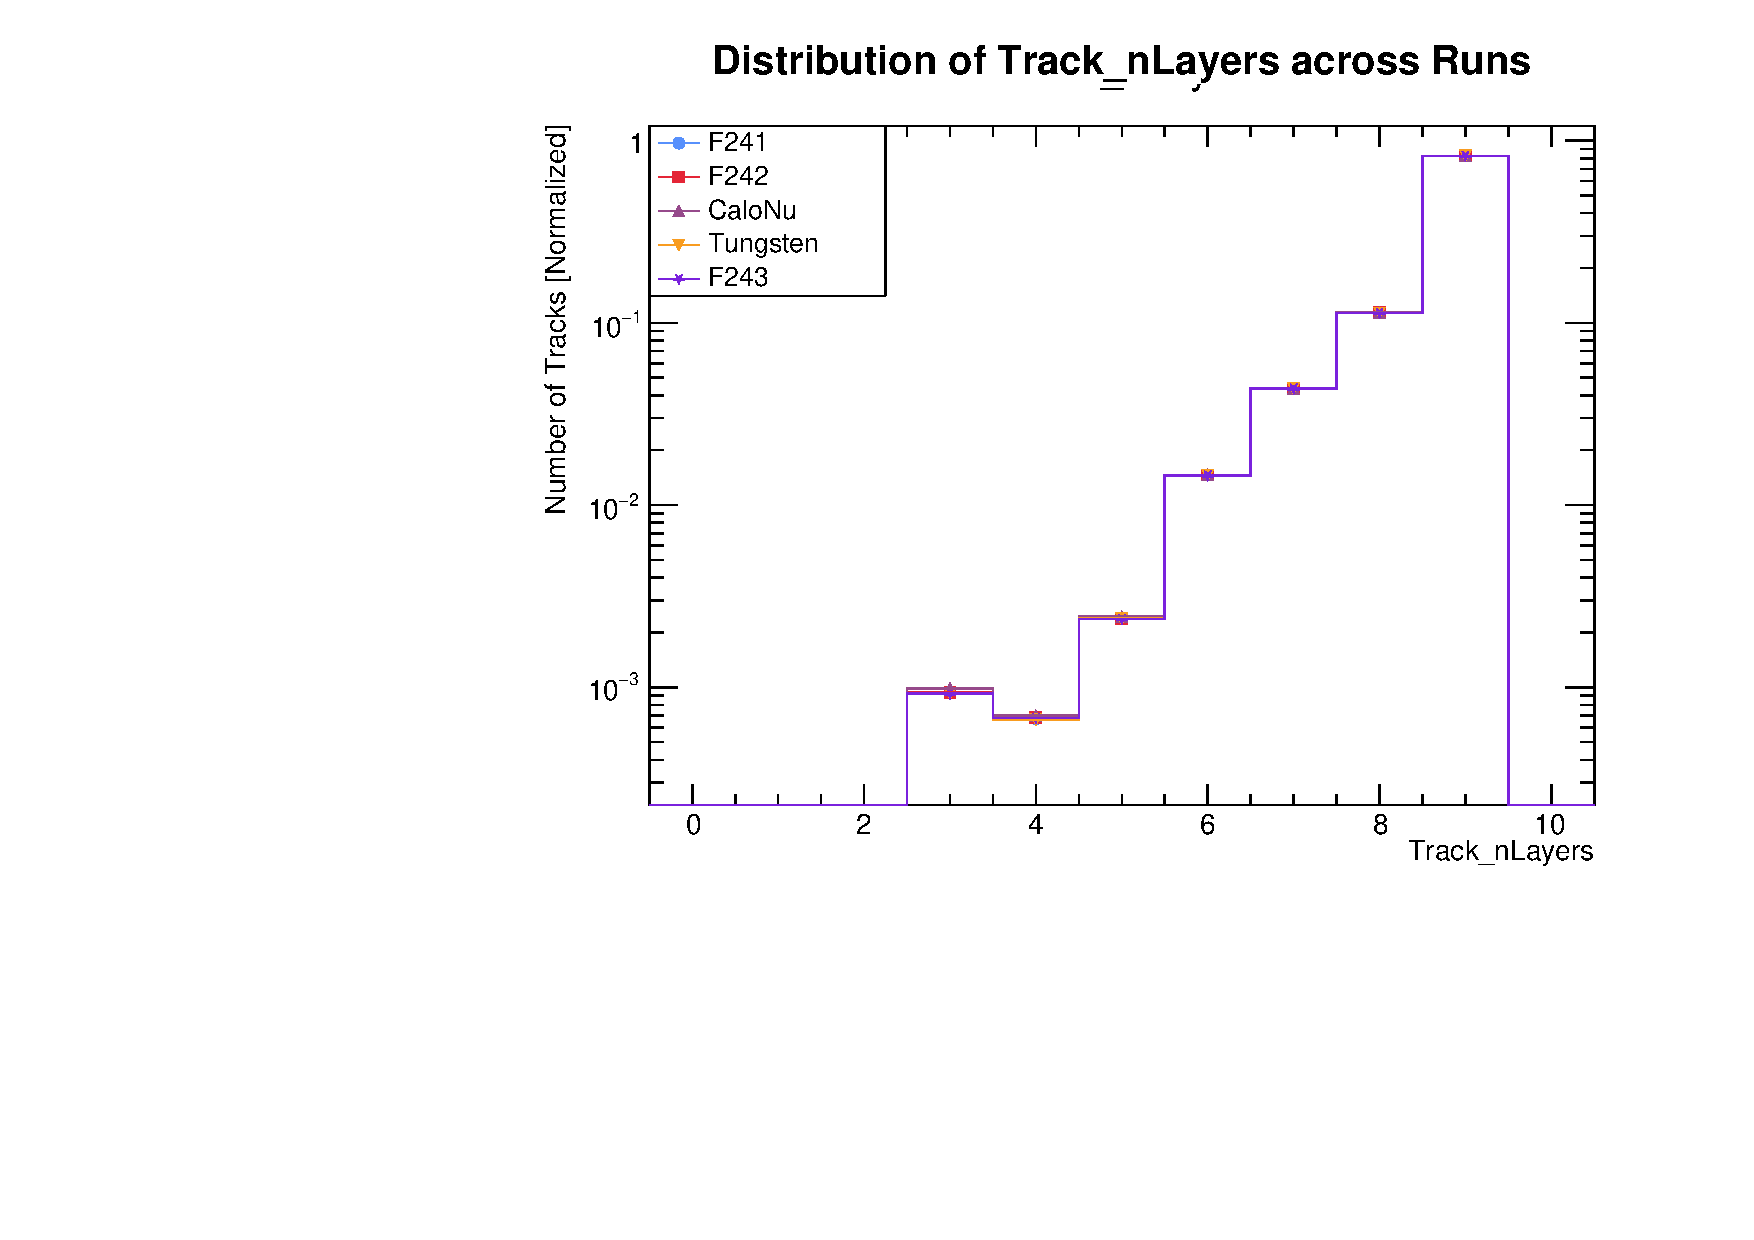
\includegraphics[width=\linewidth]{./RunwisePlots/Track_nLayers_runwise.pdf}
% 		\end{column}
% 	\end{columns}
% 	\begin{itemize}
% 		\item Really good agreement across runs for all tracking parameters across the five 2024 run periods.
% 	\end{itemize}
% \end{frame}


% \begin{frame}{Summary of Runwise Analysis}
	
% \end{frame}